\documentclass[]{article}
\usepackage{lmodern}
\usepackage{amssymb,amsmath}
\usepackage{ifxetex,ifluatex}
\usepackage{fixltx2e} % provides \textsubscript
\ifnum 0\ifxetex 1\fi\ifluatex 1\fi=0 % if pdftex
  \usepackage[T1]{fontenc}
  \usepackage[utf8]{inputenc}
\else % if luatex or xelatex
  \ifxetex
    \usepackage{mathspec}
  \else
    \usepackage{fontspec}
  \fi
  \defaultfontfeatures{Ligatures=TeX,Scale=MatchLowercase}
\fi
% use upquote if available, for straight quotes in verbatim environments
\IfFileExists{upquote.sty}{\usepackage{upquote}}{}
% use microtype if available
\IfFileExists{microtype.sty}{%
\usepackage{microtype}
\UseMicrotypeSet[protrusion]{basicmath} % disable protrusion for tt fonts
}{}
\usepackage[margin=1in]{geometry}
\usepackage{hyperref}
\hypersetup{unicode=true,
            pdftitle={Mineração de texto aplicada à Lei de Acesso à informação - LAI},
            pdfborder={0 0 0},
            breaklinks=true}
\urlstyle{same}  % don't use monospace font for urls
\usepackage{color}
\usepackage{fancyvrb}
\newcommand{\VerbBar}{|}
\newcommand{\VERB}{\Verb[commandchars=\\\{\}]}
\DefineVerbatimEnvironment{Highlighting}{Verbatim}{commandchars=\\\{\}}
% Add ',fontsize=\small' for more characters per line
\usepackage{framed}
\definecolor{shadecolor}{RGB}{248,248,248}
\newenvironment{Shaded}{\begin{snugshade}}{\end{snugshade}}
\newcommand{\KeywordTok}[1]{\textcolor[rgb]{0.13,0.29,0.53}{\textbf{#1}}}
\newcommand{\DataTypeTok}[1]{\textcolor[rgb]{0.13,0.29,0.53}{#1}}
\newcommand{\DecValTok}[1]{\textcolor[rgb]{0.00,0.00,0.81}{#1}}
\newcommand{\BaseNTok}[1]{\textcolor[rgb]{0.00,0.00,0.81}{#1}}
\newcommand{\FloatTok}[1]{\textcolor[rgb]{0.00,0.00,0.81}{#1}}
\newcommand{\ConstantTok}[1]{\textcolor[rgb]{0.00,0.00,0.00}{#1}}
\newcommand{\CharTok}[1]{\textcolor[rgb]{0.31,0.60,0.02}{#1}}
\newcommand{\SpecialCharTok}[1]{\textcolor[rgb]{0.00,0.00,0.00}{#1}}
\newcommand{\StringTok}[1]{\textcolor[rgb]{0.31,0.60,0.02}{#1}}
\newcommand{\VerbatimStringTok}[1]{\textcolor[rgb]{0.31,0.60,0.02}{#1}}
\newcommand{\SpecialStringTok}[1]{\textcolor[rgb]{0.31,0.60,0.02}{#1}}
\newcommand{\ImportTok}[1]{#1}
\newcommand{\CommentTok}[1]{\textcolor[rgb]{0.56,0.35,0.01}{\textit{#1}}}
\newcommand{\DocumentationTok}[1]{\textcolor[rgb]{0.56,0.35,0.01}{\textbf{\textit{#1}}}}
\newcommand{\AnnotationTok}[1]{\textcolor[rgb]{0.56,0.35,0.01}{\textbf{\textit{#1}}}}
\newcommand{\CommentVarTok}[1]{\textcolor[rgb]{0.56,0.35,0.01}{\textbf{\textit{#1}}}}
\newcommand{\OtherTok}[1]{\textcolor[rgb]{0.56,0.35,0.01}{#1}}
\newcommand{\FunctionTok}[1]{\textcolor[rgb]{0.00,0.00,0.00}{#1}}
\newcommand{\VariableTok}[1]{\textcolor[rgb]{0.00,0.00,0.00}{#1}}
\newcommand{\ControlFlowTok}[1]{\textcolor[rgb]{0.13,0.29,0.53}{\textbf{#1}}}
\newcommand{\OperatorTok}[1]{\textcolor[rgb]{0.81,0.36,0.00}{\textbf{#1}}}
\newcommand{\BuiltInTok}[1]{#1}
\newcommand{\ExtensionTok}[1]{#1}
\newcommand{\PreprocessorTok}[1]{\textcolor[rgb]{0.56,0.35,0.01}{\textit{#1}}}
\newcommand{\AttributeTok}[1]{\textcolor[rgb]{0.77,0.63,0.00}{#1}}
\newcommand{\RegionMarkerTok}[1]{#1}
\newcommand{\InformationTok}[1]{\textcolor[rgb]{0.56,0.35,0.01}{\textbf{\textit{#1}}}}
\newcommand{\WarningTok}[1]{\textcolor[rgb]{0.56,0.35,0.01}{\textbf{\textit{#1}}}}
\newcommand{\AlertTok}[1]{\textcolor[rgb]{0.94,0.16,0.16}{#1}}
\newcommand{\ErrorTok}[1]{\textcolor[rgb]{0.64,0.00,0.00}{\textbf{#1}}}
\newcommand{\NormalTok}[1]{#1}
\usepackage{graphicx,grffile}
\makeatletter
\def\maxwidth{\ifdim\Gin@nat@width>\linewidth\linewidth\else\Gin@nat@width\fi}
\def\maxheight{\ifdim\Gin@nat@height>\textheight\textheight\else\Gin@nat@height\fi}
\makeatother
% Scale images if necessary, so that they will not overflow the page
% margins by default, and it is still possible to overwrite the defaults
% using explicit options in \includegraphics[width, height, ...]{}
\setkeys{Gin}{width=\maxwidth,height=\maxheight,keepaspectratio}
\IfFileExists{parskip.sty}{%
\usepackage{parskip}
}{% else
\setlength{\parindent}{0pt}
\setlength{\parskip}{6pt plus 2pt minus 1pt}
}
\setlength{\emergencystretch}{3em}  % prevent overfull lines
\providecommand{\tightlist}{%
  \setlength{\itemsep}{0pt}\setlength{\parskip}{0pt}}
\setcounter{secnumdepth}{0}
% Redefines (sub)paragraphs to behave more like sections
\ifx\paragraph\undefined\else
\let\oldparagraph\paragraph
\renewcommand{\paragraph}[1]{\oldparagraph{#1}\mbox{}}
\fi
\ifx\subparagraph\undefined\else
\let\oldsubparagraph\subparagraph
\renewcommand{\subparagraph}[1]{\oldsubparagraph{#1}\mbox{}}
\fi

%%% Use protect on footnotes to avoid problems with footnotes in titles
\let\rmarkdownfootnote\footnote%
\def\footnote{\protect\rmarkdownfootnote}

%%% Change title format to be more compact
\usepackage{titling}

% Create subtitle command for use in maketitle
\providecommand{\subtitle}[1]{
  \posttitle{
    \begin{center}\large#1\end{center}
    }
}

\setlength{\droptitle}{-2em}

  \title{Mineração de texto aplicada à Lei de Acesso à informação - LAI}
    \pretitle{\vspace{\droptitle}\centering\huge}
  \posttitle{\par}
    \author{}
    \preauthor{}\postauthor{}
    \date{}
    \predate{}\postdate{}
  
\usepackage{booktabs}
\usepackage{longtable}
\usepackage{array}
\usepackage{multirow}
\usepackage{wrapfig}
\usepackage{float}
\usepackage{colortbl}
\usepackage{pdflscape}
\usepackage{tabu}
\usepackage{threeparttable}
\usepackage{threeparttablex}
\usepackage[normalem]{ulem}
\usepackage{makecell}
\usepackage{xcolor}

\begin{document}
\maketitle

\subsection{Packages for this routine}\label{packages-for-this-routine}

\section{BASE DE DADOS E ANÁLISE
EXPLORATÓRIA}\label{base-de-dados-e-analise-exploratoria}

\subsection{Importação dos dados}\label{importacao-dos-dados}

Caminho do projeto

\begin{Shaded}
\begin{Highlighting}[]
\NormalTok{PATH = }\StringTok{"..;/proj_eSIC_v10/textmining_pt/DATA/"}
\end{Highlighting}
\end{Shaded}

\subsection{Importação ee estrutura dos
dados}\label{importacao-ee-estrutura-dos-dados}

\paragraph{Tabela1: Pedidos e-SIC}\label{tabela1-pedidos-e-sic}

\begin{itemize}
\tightlist
\item
  Pedidos e-SIC
\end{itemize}

Estrutura dos dados

\begin{Shaded}
\begin{Highlighting}[]
\KeywordTok{glimpse}\NormalTok{(Pedidos_eSIC)}
\end{Highlighting}
\end{Shaded}

\begin{verbatim}
## Observations: 625
## Variables: 9
## $ Protocolo                                  <dbl> 1.685301e+16, 1.860...
## $ `Órgão Superior`                           <chr> "EPE – Empresa de P...
## $ `Data de Abertura`                         <dttm> 2017-08-19 20:26:4...
## $ `Prazo de Atendimento`                     <dttm> 2017-09-11 23:59:5...
## $ Situação                                   <chr> "Respondido", "Resp...
## $ `Descrição do Pedido`                      <chr> "A Empresa de Pesqu...
## $ `Descrição da Forma de Resposta do Pedido` <chr> "Pelo sistema (com ...
## $ `Resumo da Solicitação`                    <chr> "Empresa de Pesquis...
## $ `Data da Resposta`                         <dttm> 2017-08-30 21:19:1...
\end{verbatim}

\paragraph{Tabela2: Respostas Diretorias da
EPE}\label{tabela2-respostas-diretorias-da-epe}

\begin{itemize}
\tightlist
\item
  Respostas e-SIC (DIRETORIAS EPE)
\end{itemize}

Estrutura dos dados

\begin{Shaded}
\begin{Highlighting}[]
\KeywordTok{glimpse}\NormalTok{(Respostas_EPE)}
\end{Highlighting}
\end{Shaded}

\begin{verbatim}
## Observations: 705
## Variables: 3
## $ ProtocoloPedido                     <dbl> 9.993800e+16, 9.993800e+16...
## $ DataRegistro                        <dttm> 2015-07-24, 2015-07-28, 2...
## $ DiretoriaEPE_ResponsavelPelaDemanda <chr> "DGC", "DEA", "DEA", "DEE"...
\end{verbatim}

\paragraph{Tabela3: Stopwords}\label{tabela3-stopwords}

\begin{itemize}
\tightlist
\item
  Stopwords
\end{itemize}

\begin{Shaded}
\begin{Highlighting}[]
\NormalTok{FILE2 =}\StringTok{ "DATA/stopwords_PT_FINAL.csv"}
\NormalTok{stopwords_pt =}\StringTok{ }\KeywordTok{read.csv}\NormalTok{(}\KeywordTok{paste0}\NormalTok{(PATH,FILE2), }\DataTypeTok{sep =} \StringTok{';'}\NormalTok{, }\DataTypeTok{header =}\NormalTok{ F, }\DataTypeTok{encoding =} \StringTok{"UTF-8"}\NormalTok{)}
\NormalTok{stopwords_pt =}\StringTok{ }\NormalTok{stopwords_pt[,}\OperatorTok{-}\DecValTok{2}\NormalTok{]; }
\KeywordTok{cat}\NormalTok{(}\KeywordTok{paste0}\NormalTok{(}\StringTok{"O nosso vetor de stopwords contém "}\NormalTok{,}\KeywordTok{length}\NormalTok{(stopwords_pt), }\StringTok{" palavras únicas"}\NormalTok{))}
\end{Highlighting}
\end{Shaded}

\begin{verbatim}
## O nosso vetor de stopwords contém 704 palavras únicas
\end{verbatim}

\begin{Shaded}
\begin{Highlighting}[]
\NormalTok{## dim(stopwords_pt); class(stopwords_pt)}
\NormalTok{stopwords_pt =}\StringTok{ }\KeywordTok{as.character}\NormalTok{(stopwords_pt)}
\NormalTok{stopwords_pt[}\DecValTok{1}\OperatorTok{:}\DecValTok{14}\NormalTok{]}
\end{Highlighting}
\end{Shaded}

\begin{verbatim}
##  [1] "a"       "à"       "acerca"  "acesso"  "adeus"   "agora"   "aí"     
##  [8] "ai"      "ainda"   "alem"    "além"    "algmas"  "algo"    "algumas"
\end{verbatim}

\paragraph{Tabelas4,5,6: Dicionários de variáveis
e-SIC}\label{tabelas456-dicionarios-de-variaveis-e-sic}

\begin{itemize}
\tightlist
\item
  Dicionário \textgreater{} BASE DE DADOS - REAL PRO TEXTO DO TCC
\end{itemize}

Dicionário de variáveis - PEDIDOS

\begin{Shaded}
\begin{Highlighting}[]
\NormalTok{dicionario =}\StringTok{ "DATA/Dicionario-Dados-Exportacao.txt"}
\NormalTok{dic_pedidos =}\StringTok{ }\KeywordTok{read.delim}\NormalTok{(dicionario, }\DataTypeTok{sep =} \StringTok{"-"}\NormalTok{, }\DataTypeTok{skip =} \DecValTok{3}\NormalTok{, }\DataTypeTok{header =} \OtherTok{FALSE}\NormalTok{, }\DataTypeTok{nrows =} \DecValTok{21}\NormalTok{) }\OperatorTok
\StringTok{  }\KeywordTok{select}\NormalTok{(}\OperatorTok{-}\NormalTok{V1)}
\KeywordTok{colnames}\NormalTok{(dic_pedidos) =}\StringTok{ }\KeywordTok{c}\NormalTok{(}\StringTok{"Nome das variáveis"}\NormalTok{, }\StringTok{"Tipo e descrição da variável"}\NormalTok{)}
\CommentTok{#dimnames(dic_pedidos); View(dic_pedidos)}
\end{Highlighting}
\end{Shaded}

Dicionário de variáveis - RECURSOS

\begin{Shaded}
\begin{Highlighting}[]
\NormalTok{dic_recursos =}\StringTok{ }\KeywordTok{read.delim}\NormalTok{(dicionario, }\DataTypeTok{sep =} \StringTok{"-"}\NormalTok{, }\DataTypeTok{skip =} \DecValTok{30}\NormalTok{, }\DataTypeTok{header =} \OtherTok{FALSE}\NormalTok{, }\DataTypeTok{nrows =} \DecValTok{17}\NormalTok{) }\OperatorTok
\StringTok{  }\KeywordTok{select}\NormalTok{(}\OperatorTok{-}\NormalTok{V1)}
\KeywordTok{colnames}\NormalTok{(dic_recursos) =}\StringTok{ }\KeywordTok{c}\NormalTok{(}\StringTok{"Nome das variáveis"}\NormalTok{, }\StringTok{"Tipo e descrição da variável"}\NormalTok{)}
\CommentTok{#dimnames(dic_recursos); View(dic_recursos)}
\end{Highlighting}
\end{Shaded}

Dicionário de variáveis - SOLICITANTES

\begin{Shaded}
\begin{Highlighting}[]
\NormalTok{dicionario =}\StringTok{ "DATA/Dicionario-Dados-Exportacao.txt"}
\NormalTok{dic_solicitantes =}\StringTok{ }\KeywordTok{read.delim}\NormalTok{(}\DataTypeTok{file =}\NormalTok{ dicionario, }\DataTypeTok{sep =} \StringTok{"-"}\NormalTok{, }\DataTypeTok{skip =} \DecValTok{53}\NormalTok{, }\DataTypeTok{header =} \OtherTok{FALSE}\NormalTok{, }\DataTypeTok{nrows =} \DecValTok{10}\NormalTok{) }\OperatorTok
\StringTok{  }\KeywordTok{select}\NormalTok{(}\OperatorTok{-}\NormalTok{V1)}
\KeywordTok{colnames}\NormalTok{(dic_solicitantes) =}\StringTok{ }\KeywordTok{c}\NormalTok{(}\StringTok{"Nome das variáveis"}\NormalTok{, }\StringTok{"Tipo e descrição da variável"}\NormalTok{)}
\CommentTok{#dimnames(dic_solicitantes); View(dic_solicitantes)}
\end{Highlighting}
\end{Shaded}

\subsection{Transformação e pré-processamento dos
dados}\label{transformacao-e-pre-processamento-dos-dados}

\subsubsection{Filtra, Transforma e Unifica
bases}\label{filtra-transforma-e-unifica-bases}

\paragraph{Filtro1: tabela consulta de
pedidos}\label{filtro1-tabela-consulta-de-pedidos}

Filtrando apenas as variáveis de interesse do estudo na tabela de
consulta de pedidos

\begin{Shaded}
\begin{Highlighting}[]
\NormalTok{LAI =}\StringTok{ }\NormalTok{LAI }\OperatorTok\StringTok{ }\KeywordTok{select}\NormalTok{(Protocolo, }\StringTok{`}\DataTypeTok{Data de Abertura}\StringTok{`}\NormalTok{, }\StringTok{`}\DataTypeTok{Prazo de Atendimento}\StringTok{`}\NormalTok{, }\StringTok{`}\DataTypeTok{Descrição do Pedido}\StringTok{`}\NormalTok{, }\StringTok{`}\DataTypeTok{Resumo da Solicitação}\StringTok{`}\NormalTok{, }\StringTok{`}\DataTypeTok{Data da Resposta}\StringTok{`}\NormalTok{)}
\end{Highlighting}
\end{Shaded}

\paragraph{Transformação1: reescrevendo
colunas}\label{transformacao1-reescrevendo-colunas}

Reescrevendo o nome das variáveis de ambas tablelas

\begin{Shaded}
\begin{Highlighting}[]
\KeywordTok{colnames}\NormalTok{(LAI) =}\StringTok{ }\KeywordTok{c}\NormalTok{(}\StringTok{"Protocolo"}\NormalTok{, }\StringTok{"DATA_REGISTRO"}\NormalTok{, }\StringTok{"DATA_PRAZOATEND"}\NormalTok{, }\StringTok{"DESCRI_PEDIDO"}\NormalTok{,}
                     \StringTok{"RESUMO_PEDIDO"}\NormalTok{, }\StringTok{"DATA_RESPOSTA"}\NormalTok{)}
\KeywordTok{colnames}\NormalTok{(LAI1) =}\StringTok{ }\KeywordTok{c}\NormalTok{(}\StringTok{"Protocolo"}\NormalTok{, }\StringTok{"DATA_REGISTRO"}\NormalTok{, }\StringTok{"DIRETORIAS"}\NormalTok{)}
\end{Highlighting}
\end{Shaded}

\begin{quote}
Análise1: Quantitativo de pedidos por diretoria
\end{quote}

\paragraph{Transformação2: substitui NA por OUTROS (coluna
DIRETORIAS)}\label{transformacao2-substitui-na-por-outros-coluna-diretorias}

\begin{Shaded}
\begin{Highlighting}[]
\NormalTok{LAI1 =}\StringTok{ }
\StringTok{  }\NormalTok{LAI1 }\OperatorTok\StringTok{ }
\StringTok{  }\KeywordTok{replace_na}\NormalTok{(}\KeywordTok{list}\NormalTok{(}\DataTypeTok{DIRETORIAS =} \StringTok{"OUTROS"}\NormalTok{))}
\NormalTok{diretorias =}\StringTok{ }\KeywordTok{levels}\NormalTok{(}\KeywordTok{as.factor}\NormalTok{(LAI1}\OperatorTok{$}\NormalTok{DIRETORIAS))}
\end{Highlighting}
\end{Shaded}

\paragraph{Tabela1: Quantitativo de pedidos por diretoria - sem
reclassificação}\label{tabela1-quantitativo-de-pedidos-por-diretoria---sem-reclassificacao}

\begin{itemize}
\tightlist
\item
  Tabela 01 número de solcitações/pedidos de informação
\end{itemize}

\begin{Shaded}
\begin{Highlighting}[]
\NormalTok{pedidos_diretoria =}\StringTok{ }\NormalTok{LAI1 }\OperatorTok
\StringTok{ }\KeywordTok{count}\NormalTok{(DIRETORIAS, }\DataTypeTok{sort =} \OtherTok{TRUE}\NormalTok{, }\DataTypeTok{name =} \StringTok{"total_pedidos"}\NormalTok{) }
\NormalTok{pedidos_diretoria }\OperatorTok
\StringTok{  }\KeywordTok{kable}\NormalTok{(}\StringTok{"latex"}\NormalTok{, }\DataTypeTok{caption =} \StringTok{"Quantitativo de solicitações por Diretoria/EPE via e-SIC - sem reclassificação"}\NormalTok{, }
        \DataTypeTok{booktabs =}\NormalTok{ T) }\OperatorTok
\StringTok{  }\KeywordTok{kable_styling}\NormalTok{(}\DataTypeTok{latex_options =} \KeywordTok{c}\NormalTok{(}\StringTok{"striped"}\NormalTok{, }\StringTok{"hold_position"}\NormalTok{))}
\end{Highlighting}
\end{Shaded}

\begin{table}[!h]

\caption{\label{tab:unnamed-chunk-17}Quantitativo de solicitações por Diretoria/EPE via e-SIC - sem reclassificação}
\centering
\begin{tabular}{lr}
\toprule
DIRETORIAS & total\_pedidos\\
\midrule
\rowcolor{gray!6}  DEE & 244\\
DEA & 240\\
\rowcolor{gray!6}  DGC & 121\\
OUTROS & 67\\
\rowcolor{gray!6}  DPG & 33\\
\bottomrule
\end{tabular}
\end{table}

Verificamos a existência de 4 diretorias, sendo elas: \emph{DEA},
\emph{DEE}, \emph{DGC}, \emph{DPG} e \emph{OUTROS}. Essa última é devido
a existência de informações solicitadas que não são de competência de
nenhuma das cinco diretorias, daí a necessidade de uma última categoria
\emph{OUTROS} para atender essas demandas.

Fica nítida o desbalanceamento do número de pedidos por categoria.
Enquanto as diretorias \emph{DEE} e \emph{DEA} possuem, respectivamente,
244 e 240 pedidos verifica-se uma diferença grande do número de pedido
das diretorias \emph{DGC} e \emph{DPG} e também da categoria
\emph{OUTRAS}, onde se forem somadas possuem um total de 221 pedidos
conjuntamente.

A seguir, um passo importante de reclassificação será executado devido
ao número pequeno de solicitações para as diretorias DGC e DPG Apenas
uma solcitação existente no nosso banco de dados para essa diretoria.
Iremos, portanto, unificar essa demanda à categoria \emph{OUTROS}. A
seguir, verificamos nas tabela 01 e 02 a distribuição de pedidos por
diretoria antes e após reclassificação das mesmas.

\paragraph{Tabela1: Quantitativo de pedidos por diretoria - sem
reclassificação}\label{tabela1-quantitativo-de-pedidos-por-diretoria---sem-reclassificacao-1}

Respostas e-SIC - Reclassificação Diretorias

\begin{Shaded}
\begin{Highlighting}[]
\NormalTok{LAI1 =}\StringTok{ }\NormalTok{LAI1 }\OperatorTok\StringTok{ }
\StringTok{  }\KeywordTok{mutate}\NormalTok{(}\DataTypeTok{DIRETORIA =} \KeywordTok{ifelse}\NormalTok{(DIRETORIAS }\OperatorTok{==}\StringTok{ "DGC"}\NormalTok{, }\StringTok{"OUTROS"}\NormalTok{,}
                            \KeywordTok{ifelse}\NormalTok{(DIRETORIAS }\OperatorTok{==}\StringTok{ "DPG"}\NormalTok{, }\StringTok{"OUTROS"}\NormalTok{,DIRETORIAS)))}
\NormalTok{diretorias1 =}\StringTok{ }\KeywordTok{levels}\NormalTok{(}\KeywordTok{as.factor}\NormalTok{(LAI1}\OperatorTok{$}\NormalTok{DIRETORIA))}
\end{Highlighting}
\end{Shaded}

\paragraph{Tabela2: Quantitativo de pedidos por diretoria - após
reclassificação}\label{tabela2-quantitativo-de-pedidos-por-diretoria---apos-reclassificacao}

\begin{itemize}
\tightlist
\item
  Tabela 02 número de solcitações/pedidos de informação - após
  reclassificação
\end{itemize}

\begin{Shaded}
\begin{Highlighting}[]
\NormalTok{pedidos_diretoria1 =}\StringTok{ }\NormalTok{LAI1 }\OperatorTok
\StringTok{ }\KeywordTok{count}\NormalTok{(DIRETORIA, }\DataTypeTok{sort =} \OtherTok{TRUE}\NormalTok{, }\DataTypeTok{name =} \StringTok{"total_pedidos"}\NormalTok{) }
\NormalTok{pedidos_diretoria1 }\OperatorTok
\StringTok{  }\KeywordTok{kable}\NormalTok{(}\StringTok{"latex"}\NormalTok{, }\DataTypeTok{caption =} \StringTok{"Quantitativo de solicitações por Diretoria/EPE via e-SIC - após reclassificação"}\NormalTok{, }
        \DataTypeTok{booktabs =}\NormalTok{ T) }\OperatorTok
\StringTok{  }\KeywordTok{kable_styling}\NormalTok{(}\DataTypeTok{latex_options =} \KeywordTok{c}\NormalTok{(}\StringTok{"striped"}\NormalTok{, }\StringTok{"hold_position"}\NormalTok{))}
\end{Highlighting}
\end{Shaded}

\begin{table}[!h]

\caption{\label{tab:unnamed-chunk-19}Quantitativo de solicitações por Diretoria/EPE via e-SIC - após reclassificação}
\centering
\begin{tabular}{lr}
\toprule
DIRETORIA & total\_pedidos\\
\midrule
\rowcolor{gray!6}  DEE & 244\\
DEA & 240\\
\rowcolor{gray!6}  OUTROS & 221\\
\bottomrule
\end{tabular}
\end{table}

Temos, finalmente um maior balanceamento nas categorias da nossa
variável resposta com 244, 240 e 221 pedidos que foram destinios à
\emph{DEE}, \emph{DEA} e \emph{OUTROS}, respectivamente. Onde
\emph{OUTROS} é a categoria formada com a união dos pedidos das
diretorias \emph{DGC}, \emph{DPG} e \emph{OUTROS}.

A reclassificação foi, também, uma decisão suportada por análises
préveias do presente estudo. Foi avaliada a viabilidade de aplicar o
estudo com as categorias originais, entretanto na fase de modelagem
preditiva o desempenho do modelo do Random Forest foi muito inferior
comparado ao modelo após reclassificação. Um motivo plausível para a
melhoria de performance pode ser por conta do maior balanceamento entre
as categorias da variável resposta \textbf{Diretoria}, em questão.

\begin{itemize}
\tightlist
\item
  Unificando as Bases
\end{itemize}

É necessário, agora, unificar as bases de dados pertinentes a
solicitações e respostas.

\paragraph{Join1: União das bases em
questão}\label{join1-uniao-das-bases-em-questao}

\begin{Shaded}
\begin{Highlighting}[]
\NormalTok{LAI1 =}\StringTok{ }\NormalTok{LAI1 }\OperatorTok\StringTok{ }\KeywordTok{select}\NormalTok{(}\OperatorTok{-}\NormalTok{DATA_REGISTRO); }\CommentTok{#dim(LAI1)}
\NormalTok{DB =}\StringTok{ }\KeywordTok{left_join}\NormalTok{(}\DataTypeTok{x =}\NormalTok{ LAI, }\DataTypeTok{y =}\NormalTok{ LAI1, }\DataTypeTok{by =} \StringTok{"Protocolo"}\NormalTok{) }\OperatorTok
\StringTok{  }\KeywordTok{drop_na}\NormalTok{()}
\CommentTok{#View(head(DB))}
\end{Highlighting}
\end{Shaded}

Ver Anexo 01 c/ amostra dos dados da tabela que serpá utilizada para
manipulação daqui pra frente.

\subsection{Mineração de texto}\label{mineracao-de-texto}

\subsubsection{Palavras por pedido}\label{palavras-por-pedido}

\begin{quote}
Análise2: distribuição de frequência de palavras por diretoria e algumas
estatísticas descritivas
\end{quote}

\paragraph{Ferramentas}\label{ferramentas}

Iniciamos as manipulações utilizando recursos da função
\texttt{unnest\_tokens(\ )} do pacote \texttt{library(tidytext)} que nos
permite trabalhar com textos em um formato \texttt{tidy}, ou seja que
coloca uma palavra por linha em uma única coluna, formando, assim,
\emph{termos/palavras} por linha. Utilizamos, também, ainda os recursos
do pacote \texttt{library(diplyr)} para, posteriormente, agrupar esses
termos por diretoria e calcular a frequência dos \emph{termos}.

Verificamos que as 10 palavras mais frequentes em todos os pedidos
realizados são palavras sem acréscimo contextual, pois essas não
acrescentam nenhum sentido semântico como, por exemplo: preposições (de,
da, do, para, em, no), conjunção (e) e artigos(o,a).

Citar o que é preoposição.

\paragraph{Tabela3: Palavras mais
frequentes}\label{tabela3-palavras-mais-frequentes}

\begin{itemize}
\tightlist
\item
  Tabela 03 Palavras mais frequentes no conjunto de solicitações por
  diretoria
\end{itemize}

\begin{Shaded}
\begin{Highlighting}[]
\KeywordTok{library}\NormalTok{(tidytext)}
\NormalTok{palavras <-}\StringTok{ }\NormalTok{DB }\OperatorTok
\StringTok{  }\KeywordTok{unnest_tokens}\NormalTok{(palavra, DESCRI_PEDIDO) }\OperatorTok
\StringTok{  }\KeywordTok{count}\NormalTok{(palavra, }\DataTypeTok{sort =} \OtherTok{TRUE}\NormalTok{) }\OperatorTok
\StringTok{  }\KeywordTok{ungroup}\NormalTok{()}

\NormalTok{palavras[}\DecValTok{0}\OperatorTok{:}\DecValTok{10}\NormalTok{,] }\OperatorTok
\StringTok{  }\KeywordTok{kable}\NormalTok{(}\StringTok{"latex"}\NormalTok{, }\DataTypeTok{caption =} \StringTok{"Principais palavras com stopwords"}\NormalTok{, }
        \DataTypeTok{booktabs =}\NormalTok{ T, }\DataTypeTok{format.args =} \KeywordTok{list}\NormalTok{(}\DataTypeTok{decimal.mark =} \StringTok{','}\NormalTok{, }\DataTypeTok{big.mark =} \StringTok{"."}\NormalTok{)) }\OperatorTok
\StringTok{  }\KeywordTok{kable_styling}\NormalTok{(}\DataTypeTok{latex_options =} \KeywordTok{c}\NormalTok{(}\StringTok{"striped"}\NormalTok{, }\StringTok{"hold_position"}\NormalTok{))}
\end{Highlighting}
\end{Shaded}

\begin{table}[!h]

\caption{\label{tab:unnamed-chunk-21}Principais palavras com stopwords}
\centering
\begin{tabular}{lr}
\toprule
palavra & n\\
\midrule
\rowcolor{gray!6}  de & 3.336\\
a & 1.198\\
\rowcolor{gray!6}  e & 1.026\\
o & 845\\
\rowcolor{gray!6}  do & 752\\
\addlinespace
da & 732\\
\rowcolor{gray!6}  para & 616\\
em & 535\\
\rowcolor{gray!6}  que & 527\\
no & 497\\
\bottomrule
\end{tabular}
\end{table}

\paragraph{Tabelas4,5,6: Palavras mais frequentes por
diretoria}\label{tabelas456-palavras-mais-frequentes-por-diretoria}

\subparagraph{Tabelas4: Palavras mais frequentes
DEA}\label{tabelas4-palavras-mais-frequentes-dea}

\begin{itemize}
\tightlist
\item
  Tabela 04 Palavras mais frequentes no conjunto de solicitações por
  diretoria
\end{itemize}

\begin{Shaded}
\begin{Highlighting}[]
\NormalTok{palavras_diretoria <-}\StringTok{ }\NormalTok{DB }\OperatorTok
\StringTok{  }\KeywordTok{unnest_tokens}\NormalTok{(palavra, DESCRI_PEDIDO) }\OperatorTok
\StringTok{  }\KeywordTok{count}\NormalTok{(DIRETORIA,palavra, }\DataTypeTok{sort =} \OtherTok{TRUE}\NormalTok{) }\OperatorTok
\StringTok{  }\KeywordTok{ungroup}\NormalTok{() }\OperatorTok\StringTok{  }\KeywordTok{droplevels}\NormalTok{() }\OperatorTok\StringTok{ }\KeywordTok{drop_na}\NormalTok{()}


\NormalTok{palavras_diretoria }\OperatorTok
\StringTok{  }\KeywordTok{filter}\NormalTok{(DIRETORIA }\OperatorTok{==}\StringTok{ "DEA"}\NormalTok{) }\OperatorTok
\StringTok{    }\KeywordTok{top_n}\NormalTok{(}\DataTypeTok{n =} \DecValTok{10}\NormalTok{) }\OperatorTok
\StringTok{  }\KeywordTok{kable}\NormalTok{(}\StringTok{"latex"}\NormalTok{, }\DataTypeTok{caption =} \StringTok{"Principais palavras com stopwords (DEA)"}\NormalTok{, }
        \DataTypeTok{booktabs =}\NormalTok{ T, }\DataTypeTok{format.args =} \KeywordTok{list}\NormalTok{(}\DataTypeTok{decimal.mark =} \StringTok{','}\NormalTok{, }\DataTypeTok{big.mark =} \StringTok{"."}\NormalTok{)) }\OperatorTok
\StringTok{  }\KeywordTok{kable_styling}\NormalTok{(}\DataTypeTok{latex_options =} \KeywordTok{c}\NormalTok{(}\StringTok{"striped"}\NormalTok{, }\StringTok{"hold_position"}\NormalTok{))}
\end{Highlighting}
\end{Shaded}

\begin{verbatim}
## Selecting by n
\end{verbatim}

\begin{table}[!h]

\caption{\label{tab:unnamed-chunk-22}Principais palavras com stopwords (DEA)}
\centering
\begin{tabular}{llr}
\toprule
DIRETORIA & palavra & n\\
\midrule
\rowcolor{gray!6}  DEA & de & 1.193\\
DEA & a & 367\\
\rowcolor{gray!6}  DEA & e & 331\\
DEA & o & 276\\
\rowcolor{gray!6}  DEA & do & 256\\
\addlinespace
DEA & da & 226\\
\rowcolor{gray!6}  DEA & dados & 210\\
DEA & energia & 210\\
\rowcolor{gray!6}  DEA & para & 210\\
DEA & no & 206\\
\bottomrule
\end{tabular}
\end{table}

\subparagraph{Tabelas5: Palavras mais frequentes
DEE}\label{tabelas5-palavras-mais-frequentes-dee}

\begin{itemize}
\tightlist
\item
  Tabela 05 Palavras mais frequentes no conjunto de solicitações por
  diretoria
\end{itemize}

\begin{Shaded}
\begin{Highlighting}[]
\NormalTok{palavras_diretoria }\OperatorTok
\StringTok{  }\KeywordTok{filter}\NormalTok{(DIRETORIA }\OperatorTok{==}\StringTok{ "DEE"}\NormalTok{) }\OperatorTok
\StringTok{    }\KeywordTok{top_n}\NormalTok{(}\DataTypeTok{n =} \DecValTok{10}\NormalTok{) }\OperatorTok
\StringTok{  }\KeywordTok{kable}\NormalTok{(}\StringTok{"latex"}\NormalTok{, }\DataTypeTok{caption =} \StringTok{"Principais palavras com stopwords (DEA)"}\NormalTok{, }
        \DataTypeTok{booktabs =}\NormalTok{ T, }\DataTypeTok{format.args =} \KeywordTok{list}\NormalTok{(}\DataTypeTok{decimal.mark =} \StringTok{','}\NormalTok{, }\DataTypeTok{big.mark =} \StringTok{"."}\NormalTok{)) }\OperatorTok
\StringTok{  }\KeywordTok{kable_styling}\NormalTok{(}\DataTypeTok{latex_options =} \KeywordTok{c}\NormalTok{(}\StringTok{"striped"}\NormalTok{, }\StringTok{"hold_position"}\NormalTok{))}
\end{Highlighting}
\end{Shaded}

\begin{verbatim}
## Selecting by n
\end{verbatim}

\begin{table}[!h]

\caption{\label{tab:unnamed-chunk-23}Principais palavras com stopwords (DEA)}
\centering
\begin{tabular}{llr}
\toprule
DIRETORIA & palavra & n\\
\midrule
\rowcolor{gray!6}  DEE & de & 998\\
DEE & a & 367\\
\rowcolor{gray!6}  DEE & e & 283\\
DEE & do & 260\\
\rowcolor{gray!6}  DEE & o & 248\\
\addlinespace
DEE & da & 236\\
\rowcolor{gray!6}  DEE & para & 215\\
DEE & que & 156\\
\rowcolor{gray!6}  DEE & energia & 155\\
DEE & no & 153\\
\bottomrule
\end{tabular}
\end{table}

\subparagraph{Tabelas6: Palavras mais frequentes
DEA}\label{tabelas6-palavras-mais-frequentes-dea}

\begin{itemize}
\tightlist
\item
  Tabela 06 Palavras mais frequentes no conjunto de solicitações por
  diretoria
\end{itemize}

\begin{Shaded}
\begin{Highlighting}[]
\NormalTok{palavras_diretoria }\OperatorTok
\StringTok{  }\KeywordTok{filter}\NormalTok{(DIRETORIA }\OperatorTok{==}\StringTok{ "OUTROS"}\NormalTok{) }\OperatorTok
\StringTok{    }\KeywordTok{top_n}\NormalTok{(}\DataTypeTok{n =} \DecValTok{10}\NormalTok{) }\OperatorTok
\StringTok{  }\KeywordTok{kable}\NormalTok{(}\StringTok{"latex"}\NormalTok{, }\DataTypeTok{caption =} \StringTok{"Principais palavras com stopwords (OUTROS)"}\NormalTok{, }
        \DataTypeTok{booktabs =}\NormalTok{ T, }\DataTypeTok{format.args =} \KeywordTok{list}\NormalTok{(}\DataTypeTok{decimal.mark =} \StringTok{','}\NormalTok{, }\DataTypeTok{big.mark =} \StringTok{"."}\NormalTok{)) }\OperatorTok
\StringTok{  }\KeywordTok{kable_styling}\NormalTok{(}\DataTypeTok{latex_options =} \KeywordTok{c}\NormalTok{(}\StringTok{"striped"}\NormalTok{, }\StringTok{"hold_position"}\NormalTok{))}
\end{Highlighting}
\end{Shaded}

\begin{verbatim}
## Selecting by n
\end{verbatim}

\begin{table}[!h]

\caption{\label{tab:unnamed-chunk-24}Principais palavras com stopwords (OUTROS)}
\centering
\begin{tabular}{llr}
\toprule
DIRETORIA & palavra & n\\
\midrule
\rowcolor{gray!6}  OUTROS & de & 1.145\\
OUTROS & a & 464\\
\rowcolor{gray!6}  OUTROS & e & 412\\
OUTROS & o & 321\\
\rowcolor{gray!6}  OUTROS & da & 270\\
\addlinespace
OUTROS & do & 236\\
\rowcolor{gray!6}  OUTROS & que & 197\\
OUTROS & em & 196\\
\rowcolor{gray!6}  OUTROS & para & 191\\
OUTROS & ou & 171\\
\bottomrule
\end{tabular}
\end{table}

Mesmo assim, abrindo para cada uma das 3 possíveis cateogorias da
variável \textbf{Diretoria} temos que as principais palavras não agregam
nenhum valor semântico, exceto pela palavra energia que apareceu na
oitava e nona colocação de maior frequência dos documentos de pedidos
enviados à \emph{DEA} e \emph{DEE}, respectivamente. Isso devido ao
excesso de uso de \textbf{stop words} em textos humanos.

Nos passos seguintes iremos remover essas palavras, \textbf{stop words},
e trabalhar apenas com palavras de sentido semântico relevante aos
subjetivos solicitados às diretorias, acrescentando assim maior
assertividade na classificação do nosso modelo, objetivo principal desse
estudo.

Verificamos, antes disso, o total, freq. e média de palavras por
diretoria, bem como comparações 2 a 2 para cada uma das categorias.

\subsubsection{Análise2: Comparação de freq. de palavras por
diretoria}\label{analise2-comparacao-de-freq.-de-palavras-por-diretoria}

\begin{itemize}
\tightlist
\item
  Total de palavras por diretoria, total de pedidos por diretoria e
  número médio de palavras por pedido e diretoria
\end{itemize}

\begin{Shaded}
\begin{Highlighting}[]
\NormalTok{total_palavras =}\StringTok{ }\NormalTok{palavras_diretoria }\OperatorTok
\StringTok{  }\KeywordTok{group_by}\NormalTok{(DIRETORIA) }\OperatorTok
\StringTok{  }\KeywordTok{summarize}\NormalTok{(}\DataTypeTok{total_palavras =} \KeywordTok{sum}\NormalTok{(n))}

\NormalTok{total_palavras =}\StringTok{ }\KeywordTok{left_join}\NormalTok{(}\DataTypeTok{x =}\NormalTok{ total_palavras, }\DataTypeTok{y =}\NormalTok{ pedidos_diretoria1, }
                           \DataTypeTok{by =} \StringTok{"DIRETORIA"}\NormalTok{) }\OperatorTok
\KeywordTok{mutate}\NormalTok{(}\DataTypeTok{media_palavras_porpedidoEdiretoria =}\NormalTok{ total_palavras}\OperatorTok{/}\NormalTok{total_pedidos)}
\end{Highlighting}
\end{Shaded}

\paragraph{Tabelas7: Total de palavras por diretoria, total de pedidos
por diretoria e número médio de palavras por pedido e
diretoria}\label{tabelas7-total-de-palavras-por-diretoria-total-de-pedidos-por-diretoria-e-numero-medio-de-palavras-por-pedido-e-diretoria}

\begin{itemize}
\tightlist
\item
  Total de palavras por diretoria, total de pedidos por diretoria e
  número médio de palavras por pedido e diretoria
\end{itemize}

\begin{Shaded}
\begin{Highlighting}[]
\NormalTok{total_palavras }\OperatorTok
\StringTok{  }\KeywordTok{kable}\NormalTok{(}\StringTok{"latex"}\NormalTok{, }\DataTypeTok{caption =} \StringTok{"Total de palavras, total de pedidos e número médio de palavras}
\StringTok{        por pedido e diretoria"}\NormalTok{, }
        \DataTypeTok{booktabs =}\NormalTok{ T, }\DataTypeTok{format.args =} \KeywordTok{list}\NormalTok{(}\DataTypeTok{decimal.mark =} \StringTok{','}\NormalTok{, }\DataTypeTok{big.mark =} \StringTok{"."}\NormalTok{)) }\OperatorTok
\StringTok{  }\KeywordTok{kable_styling}\NormalTok{(}\DataTypeTok{latex_options =} \KeywordTok{c}\NormalTok{(}\StringTok{"striped"}\NormalTok{, }\StringTok{"hold_position"}\NormalTok{))}
\end{Highlighting}
\end{Shaded}

\begin{table}[!h]

\caption{\label{tab:unnamed-chunk-26}Total de palavras, total de pedidos e número médio de palavras
        por pedido e diretoria}
\centering
\begin{tabular}{lrrr}
\toprule
DIRETORIA & total\_palavras & total\_pedidos & media\_palavras\_porpedidoEdiretoria\\
\midrule
\rowcolor{gray!6}  DEA & 14.808 & 240 & 61,70000\\
DEE & 13.429 & 244 & 55,03689\\
\rowcolor{gray!6}  OUTROS & 15.395 & 221 & 69,66063\\
\bottomrule
\end{tabular}
\end{table}

Temos que o número médio de palavras por pedido é parecido entre as
diretorias. com médias de 55 palavras por pedido para DEE e 69,7 e 61,7,
respectivamente para DEA e OUTROS.

\paragraph{Figura1: Distribuição de frequência de termos por
diretoria}\label{figura1-distribuicao-de-frequencia-de-termos-por-diretoria}

\begin{itemize}
\tightlist
\item
  Distribuição da freq. de palavras usadas em solicitações por diretoria
  (histograma)
\end{itemize}

\begin{Shaded}
\begin{Highlighting}[]
\NormalTok{diretoria_palavras <-}\StringTok{ }\NormalTok{DB }\OperatorTok
\StringTok{  }\KeywordTok{unnest_tokens}\NormalTok{(palavra, DESCRI_PEDIDO) }\OperatorTok
\StringTok{  }\KeywordTok{count}\NormalTok{(DIRETORIA, palavra, }\DataTypeTok{sort =} \OtherTok{TRUE}\NormalTok{) }\OperatorTok
\StringTok{  }\KeywordTok{ungroup}\NormalTok{()}

\NormalTok{diretoria_palavras =}\StringTok{ }\KeywordTok{left_join}\NormalTok{(diretoria_palavras, total_palavras, }\DataTypeTok{by =} \StringTok{"DIRETORIA"}\NormalTok{)}

\KeywordTok{library}\NormalTok{(ggplot2)}
\NormalTok{gcomma <-}\StringTok{ }\ControlFlowTok{function}\NormalTok{(x) }\KeywordTok{format}\NormalTok{(x, }\DataTypeTok{big.mark =} \StringTok{"."}\NormalTok{, }\DataTypeTok{decimal.mark =} \StringTok{","}\NormalTok{, }\DataTypeTok{scientific =} \OtherTok{FALSE}\NormalTok{)}

\KeywordTok{ggplot}\NormalTok{(diretoria_palavras, }\KeywordTok{aes}\NormalTok{(n}\OperatorTok{/}\NormalTok{total_palavras, }\DataTypeTok{fill =}\NormalTok{ DIRETORIA)) }\OperatorTok{+}\StringTok{ }
\StringTok{  }\KeywordTok{geom_histogram}\NormalTok{(}\DataTypeTok{show.legend =} \OtherTok{FALSE}\NormalTok{) }\OperatorTok{+}\StringTok{ }\KeywordTok{xlim}\NormalTok{(}\OtherTok{NA}\NormalTok{, }\FloatTok{0.0021}\NormalTok{) }\OperatorTok{+}
\KeywordTok{facet_wrap}\NormalTok{(}\OperatorTok{~}\NormalTok{DIRETORIA, }\DataTypeTok{ncol =} \DecValTok{2}\NormalTok{, }\DataTypeTok{scales =} \StringTok{"free_y"}\NormalTok{) }\OperatorTok{+}\StringTok{ }
\StringTok{  }\KeywordTok{scale_y_continuous}\NormalTok{(}\DataTypeTok{labels=}\NormalTok{gcomma)  }\OperatorTok{+}
\StringTok{  }\KeywordTok{scale_x_continuous}\NormalTok{(}\DataTypeTok{labels=}\NormalTok{gcomma, }\DataTypeTok{limits =} \KeywordTok{c}\NormalTok{(}\OtherTok{NA}\NormalTok{, }\FloatTok{0.0021}\NormalTok{))}
\end{Highlighting}
\end{Shaded}

\begin{verbatim}
## Scale for 'x' is already present. Adding another scale for 'x', which
## will replace the existing scale.
\end{verbatim}

\begin{verbatim}
## `stat_bin()` using `bins = 30`. Pick better value with `binwidth`.
\end{verbatim}

\begin{verbatim}
## Warning: Removed 175 rows containing non-finite values (stat_bin).
\end{verbatim}

\begin{verbatim}
## Warning: Removed 3 rows containing missing values (geom_bar).
\end{verbatim}

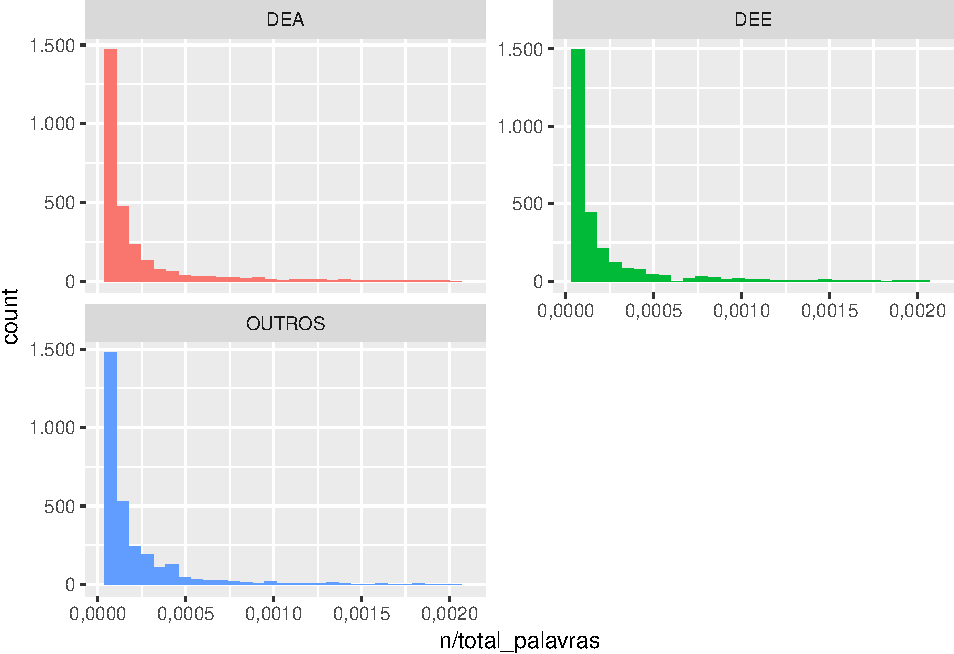
\includegraphics{markdown_v40_test_files/figure-latex/unnamed-chunk-27-1.pdf}

Pelos histogramas fica claro que as distribuições da frequência de
termos por diretoria possuem caudas mais alongadas à direita, isso sem
contar algumas frequências que não foram evidenciadas nessas figuras por
questões de escala, do contrário seria possível, apenas, ver a
frequência das palavras mais recorrentes no texto que, como vimos até o
momento, são as de menor relevância em contexto e semântica.

Sabemos, portanto, que queremos encontrar valor exatamente nas partes
mais longas à direita das distribuições de frequência de termos, uma vez
que ali se encontram as palavras de maior valor contextual.

Logo, a seguir, usamos da definição da lei \textbf{Zipf} que afirma que
a frequência que uma palavra (ou termo) aparece em um documento é
inversamente proporcional ao seu ranque.

\begin{quote}
lei de Zipf's
\end{quote}

Citar, aqui, ``There are very long tails to the right for these novels
(those extremely common words!) that we have not shown in these plots.
These plots exhibit similar distributions for all the novels, with many
words that occur rarely and fewer words that occur frequently.'' pág. 31
(Silge, Robinson). Que averigua que documentos de texto tendem a ter
distribuições de frequência de palavras similar, por conta das
stopwords.

Ainda de acordo com os autores, ``Distributions like those shown in
Figure 3-1 are typical in language. In fact, those types of long-tailed
distributions are so common in any given corpus of natural lan‐ guage
(like a book, or a lot of text from a website, or spoken words) that the
relation‐ ship between the frequency that a word is used and its rank
has been the subject of study.'' e por essa razão e a relação verificada
por George Zipf da relação inversa entre freq. de palavra e ranque
tiramos valor dos documentos partindo dessas premissas.

\begin{itemize}
\tightlist
\item
  Ranque de palavras pela pela lei de \textbf{Zipf}
\end{itemize}

\begin{Shaded}
\begin{Highlighting}[]
\NormalTok{freq_by_rank <-}\StringTok{ }\NormalTok{diretoria_palavras }\OperatorTok
\KeywordTok{group_by}\NormalTok{(DIRETORIA) }\OperatorTok
\KeywordTok{mutate}\NormalTok{(}\DataTypeTok{ranque =} \KeywordTok{row_number}\NormalTok{(),}
\StringTok{`}\DataTypeTok{frequência de termos}\StringTok{`}\NormalTok{ =}\StringTok{ }\NormalTok{n}\OperatorTok{/}\NormalTok{total_palavras)}
\end{Highlighting}
\end{Shaded}

\paragraph{Figura1: Lei de Zipf}\label{figura1-lei-de-zipf}

\begin{itemize}
\tightlist
\item
  Zipf's law
\end{itemize}

\begin{Shaded}
\begin{Highlighting}[]
\CommentTok{#plot1}
\NormalTok{freq_by_rank }\OperatorTok
\KeywordTok{ggplot}\NormalTok{(}\KeywordTok{aes}\NormalTok{(ranque, }\StringTok{`}\DataTypeTok{frequência de termos}\StringTok{`}\NormalTok{, }\DataTypeTok{color =}\NormalTok{ DIRETORIA)) }\OperatorTok{+}
\StringTok{  }\KeywordTok{geom_line}\NormalTok{(}\DataTypeTok{size =} \FloatTok{1.1}\NormalTok{, }\DataTypeTok{alpha =} \FloatTok{0.8}\NormalTok{, }\DataTypeTok{show.legend =} \OtherTok{FALSE}\NormalTok{) }\OperatorTok{+}\StringTok{ }\KeywordTok{scale_x_log10}\NormalTok{() }\OperatorTok{+}
\StringTok{  }\KeywordTok{scale_y_log10}\NormalTok{()}
\end{Highlighting}
\end{Shaded}

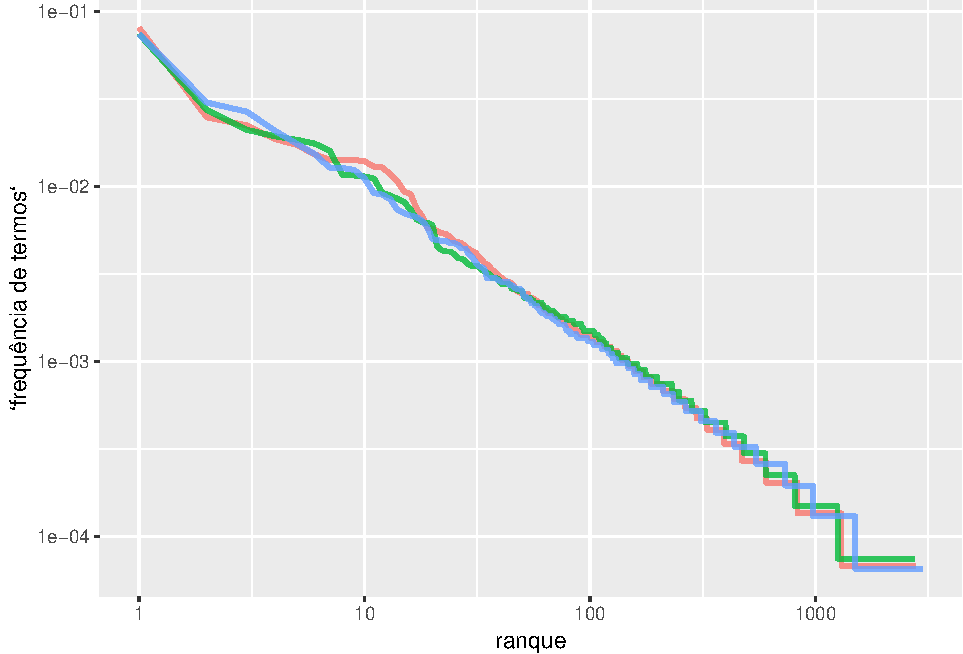
\includegraphics{markdown_v40_test_files/figure-latex/unnamed-chunk-29-1.pdf}

Vemos que exatamente nas extremidades do gráfico tem-se uma não
sobreposição de frequências por diretoria. Detalhe que o gráfico, em
questão, está na escala logarítmica no eixo x (ranque) e eixo y (freq.
de termos). Plotando desta forma, a relação inversamente proporcional
terá uma inclinação constante e negativa.

Tendo em vista, portanto, que o gráfico referido está em cordenadas
log-log e dado a semelhança de todos os documentos de texto das
diferentes diretorias, afirmamos que para todas as diretorias pela Lei
de \textbf{Zipf} a relação entre ranque e freq. de termos assumirá,
sempre, uma inclinação negativa, ou seja,

Daí, aplicando a escala log-log temos que e podemos aplicar um ajuste a
fim de encontrar um intercepto e coef. angular para traçar no gráfico
anterior.

\[
frequência \propto \frac{1}{ranque} \implies log(frequência) \propto log\left(\frac{1}{ranque}\right)
\]

Reescrever e exlicar a seguimentação em 3 partes como uma ``lei de
potenciacao dividida em 3 partes'' e então utilizar do seguimento do
meio, onde as freq. de ternos sao mais semelhantes para diferentes
ranques das diferentes diretorias. Fica claro pela eq.

``Notice that Figure 3-2 is in log-log coordinates. We see that all six
of Jane Austen's novels are similar to each other, and that the
relationship between rank and fre‐ quency does have negative slope. It
is not quite constant, though; perhaps we could view this as a broken
power law with, say, three sections. Let's see what the exponent of the
power law is for the middle section of the rank range.''

\begin{Shaded}
\begin{Highlighting}[]
\NormalTok{rank_subset <-}\StringTok{ }\NormalTok{freq_by_rank }\OperatorTok
\StringTok{      }\KeywordTok{filter}\NormalTok{(ranque }\OperatorTok{<}\StringTok{ }\DecValTok{500}\NormalTok{, ranque }\OperatorTok{>}\StringTok{ }\DecValTok{50}\NormalTok{)}

\NormalTok{(zipf_ajusteloglog <-}\StringTok{ }\KeywordTok{lm}\NormalTok{(}\KeywordTok{log10}\NormalTok{(}\StringTok{`}\DataTypeTok{frequência de termos}\StringTok{`}\NormalTok{) }\OperatorTok{~}\StringTok{ }\KeywordTok{log10}\NormalTok{(ranque), }
                         \DataTypeTok{data =}\NormalTok{ rank_subset))}
\end{Highlighting}
\end{Shaded}

\begin{verbatim}
## 
## Call:
## lm(formula = log10(`frequência de termos`) ~ log10(ranque), 
##     data = rank_subset)
## 
## Coefficients:
##   (Intercept)  log10(ranque)  
##       -1.0419        -0.9112
\end{verbatim}

Finalmente, traçando e sobrepondo o gráfico anterior com os valores de
initercepto e coeficiente angular obtidos no ajuste do passo anterior
temos a figura a seguir.

\paragraph{Figura1: Lei de Zipf + ajuste
log-log}\label{figura1-lei-de-zipf-ajuste-log-log}

\begin{Shaded}
\begin{Highlighting}[]
\NormalTok{freq_by_rank }\OperatorTok
\KeywordTok{ggplot}\NormalTok{(}\KeywordTok{aes}\NormalTok{(ranque, }\StringTok{`}\DataTypeTok{frequência de termos}\StringTok{`}\NormalTok{, }\DataTypeTok{color =}\NormalTok{ DIRETORIA)) }\OperatorTok{+}
\KeywordTok{geom_abline}\NormalTok{(}\DataTypeTok{intercept =} \KeywordTok{coefficients}\NormalTok{(zipf_ajusteloglog)[}\DecValTok{1}\NormalTok{], }\DataTypeTok{slope =} \KeywordTok{coefficients}\NormalTok{(zipf_ajusteloglog)[}\DecValTok{2}\NormalTok{], }\DataTypeTok{color =} \StringTok{"gray50"}\NormalTok{, }\DataTypeTok{linetype =} \DecValTok{2}\NormalTok{) }\OperatorTok{+}
\KeywordTok{geom_line}\NormalTok{(}\DataTypeTok{size =} \FloatTok{1.1}\NormalTok{, }\DataTypeTok{alpha =} \FloatTok{0.8}\NormalTok{, }\DataTypeTok{show.legend =} \OtherTok{TRUE}\NormalTok{) }\OperatorTok{+}
\KeywordTok{scale_x_log10}\NormalTok{(}\DataTypeTok{labels=}\NormalTok{gcomma) }\OperatorTok{+}
\KeywordTok{scale_y_log10}\NormalTok{(}\DataTypeTok{labels=}\NormalTok{gcomma)}
\end{Highlighting}
\end{Shaded}

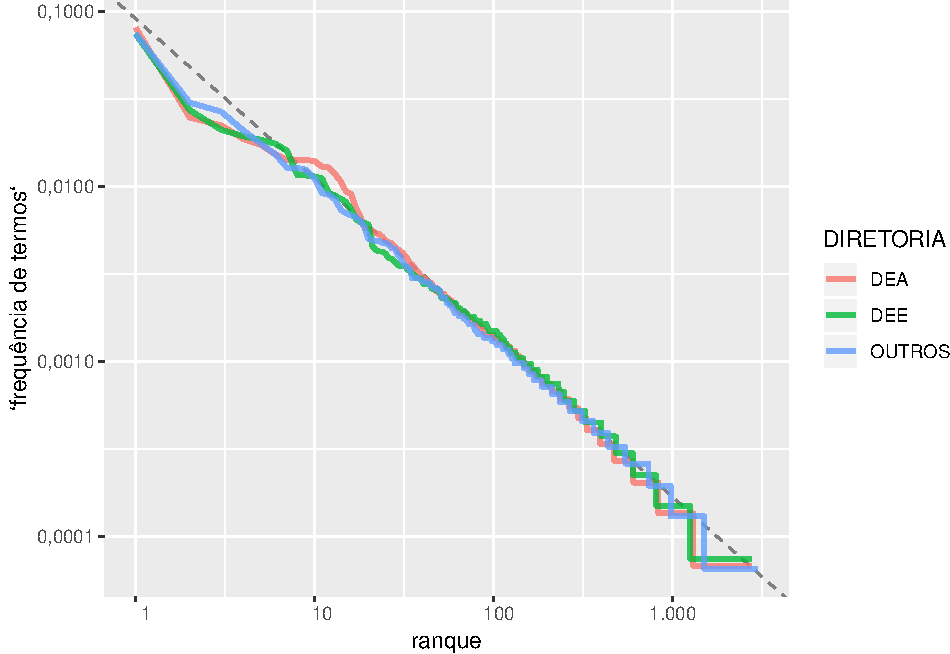
\includegraphics{markdown_v40_test_files/figure-latex/unnamed-chunk-31-1.pdf}

\paragraph{\texorpdfstring{The Bind
\textbf{tf\_idf}}{The Bind tf\_idf}}\label{the-bind-tf_idf}

Fundamentar o uso da estatística \textbf{tf\_idf}, bem como descrever a
definição.

\begin{quote}
The idea of tf-idf is to find the important words for the content of
each document by decreasing the weight for commonly used words and
increasing the weight for words that are not used very much in a
collection or corpus of documents, in this case, the group of Jane
Austen's novels as a whole. Calculating tf-idf attempts to find the
words that are important (i.e., common) in a text, but not too common.
Let's do that now. The bind\_tf\_idf function in the tidytext package
takes a tidy text dataset as input with one row per token (term), per
document. One column (word here) contains the terms/tokens, one column
contains the documents (book in this case), and the last necessary
column contains the counts, or how many times each document contains
each term (n in this example). We calculated a total for each book for
our explora‐ tions in previous sections, but it is not necessary for the
bind\_tf\_idf function; the table only needs to contain all the words in
each document.
\end{quote}

\begin{Shaded}
\begin{Highlighting}[]
\NormalTok{round_df <-}\StringTok{ }\ControlFlowTok{function}\NormalTok{(x, digits) \{}
    \CommentTok{# round all numeric variables}
    \CommentTok{# x: data frame }
    \CommentTok{# digits: number of digits to round}
\NormalTok{    numeric_columns <-}\StringTok{ }\KeywordTok{sapply}\NormalTok{(x, mode) }\OperatorTok{==}\StringTok{ 'numeric'}
\NormalTok{    x[numeric_columns] <-}\StringTok{  }\KeywordTok{round}\NormalTok{(x[numeric_columns], digits)}
\NormalTok{    x}
\NormalTok{\}}
\end{Highlighting}
\end{Shaded}

\begin{itemize}
\tightlist
\item
  Palavras mais relevantes de acordo com a estatística \textbf{tf\_idf}
\end{itemize}

\begin{Shaded}
\begin{Highlighting}[]
\NormalTok{diretoria_palavras_tfidf <-}\StringTok{ }\NormalTok{diretoria_palavras }\OperatorTok
\StringTok{  }\KeywordTok{bind_tf_idf}\NormalTok{(palavra, DIRETORIA, n) }\OperatorTok
\StringTok{  }\KeywordTok{select}\NormalTok{(}\OperatorTok{-}\NormalTok{total_palavras, }\OperatorTok{-}\NormalTok{total_pedidos, }\OperatorTok{-}\NormalTok{media_palavras_porpedidoEdiretoria) }\OperatorTok
\StringTok{  }\KeywordTok{arrange}\NormalTok{(}\KeywordTok{desc}\NormalTok{(tf_idf))}

\CommentTok{#options(digits=4)}
\KeywordTok{set.seed}\NormalTok{(}\DecValTok{7456}\NormalTok{)}
\NormalTok{amostra1 =}\StringTok{ }\KeywordTok{sample}\NormalTok{(}\KeywordTok{seq}\NormalTok{(}\DecValTok{1}\OperatorTok{:}\KeywordTok{dim}\NormalTok{(diretoria_palavras_tfidf)[}\DecValTok{1}\NormalTok{]), }\DecValTok{10}\NormalTok{, }\DataTypeTok{replace =} \OtherTok{FALSE}\NormalTok{)}
\KeywordTok{round_df}\NormalTok{(diretoria_palavras_tfidf[amostra1,],}\DecValTok{5}\NormalTok{) }\CommentTok{# %>%}
\end{Highlighting}
\end{Shaded}

\begin{verbatim}
## # A tibble: 10 x 6
##    DIRETORIA palavra          n       tf   idf   tf_idf
##    <chr>     <chr>        <dbl>    <dbl> <dbl>    <dbl>
##  1 DEA       oil              2 0.000140 1.10  0.000150
##  2 DEE       obrigado        31 0.00231  0     0       
##  3 DEE       cópias           1 0.000070 0     0       
##  4 DEE       pelos            5 0.00037  0     0       
##  5 OUTROS    suas             5 0.00032  0.405 0.000130
##  6 OUTROS    cabe             1 0.00006  0.405 0.00003 
##  7 DEE       ifsul            1 0.000070 1.10  0.00008 
##  8 OUTROS    estabelecida     1 0.00006  1.10  0.000070
##  9 DEE       valor           10 0.00074  0     0       
## 10 DEE       rica             1 0.000070 0.405 0.00003
\end{verbatim}

\begin{Shaded}
\begin{Highlighting}[]
  \KeywordTok{kable}\NormalTok{(}\StringTok{"latex"}\NormalTok{, }\DataTypeTok{caption =} \StringTok{"Total de palavras, total de pedidos e número médio de palavras }
\StringTok{        por pedido e diretoria"}\NormalTok{, }
        \DataTypeTok{booktabs =}\NormalTok{ T, }\DataTypeTok{format.args =} \KeywordTok{list}\NormalTok{(}\DataTypeTok{decimal.mark =} \StringTok{','}\NormalTok{, }\DataTypeTok{big.mark =} \StringTok{"."}\NormalTok{)) }\OperatorTok
\StringTok{  }\KeywordTok{kable_styling}\NormalTok{(}\DataTypeTok{latex_options =} \KeywordTok{c}\NormalTok{(}\StringTok{"striped"}\NormalTok{, }\StringTok{"hold_position"}\NormalTok{))}
\end{Highlighting}
\end{Shaded}

\begin{table}[!h]

\caption{\label{tab:unnamed-chunk-33}Total de palavras, total de pedidos e número médio de palavras 
        por pedido e diretoria}
\centering
\begin{tabular}{l}
\toprule
x\\
\midrule
\rowcolor{gray!6}  latex\\
\bottomrule
\end{tabular}
\end{table}

A estatística faz um trabalho brilhante ao ressaltar as palavras mais
relevantes dentro de cada conjunto de documentos (diretorias). As
tabelas a seguir mostram as 10 palavras mais relevantes de acordo com a
estatística tf\_idf por diretoria

\subparagraph{\texorpdfstring{Tabela8: top 12 termos ordenados pela
estatística \textbf{tf\_idf}
(DEE)}{Tabela8: top 12 termos ordenados pela estatística tf\_idf (DEE)}}\label{tabela8-top-12-termos-ordenados-pela-estatistica-tf_idf-dee}

\begin{Shaded}
\begin{Highlighting}[]
\KeywordTok{round_df}\NormalTok{(diretoria_palavras_tfidf,}\DecValTok{5}\NormalTok{) }\OperatorTok
\StringTok{  }\KeywordTok{filter}\NormalTok{(DIRETORIA }\OperatorTok{==}\StringTok{ "DEE"}\NormalTok{) }\OperatorTok
\StringTok{  }\KeywordTok{top_n}\NormalTok{(}\DecValTok{12}\NormalTok{,tf_idf) }\OperatorTok
\StringTok{  }\KeywordTok{kable}\NormalTok{(}\StringTok{"latex"}\NormalTok{, }\DataTypeTok{caption =} \StringTok{"Top 10 termos (DEE)"}\NormalTok{, }
        \DataTypeTok{booktabs =}\NormalTok{ T, }\DataTypeTok{format.args =} \KeywordTok{list}\NormalTok{(}\DataTypeTok{decimal.mark =} \StringTok{','}\NormalTok{, }\DataTypeTok{big.mark =} \StringTok{"."}\NormalTok{)) }\OperatorTok
\StringTok{  }\KeywordTok{kable_styling}\NormalTok{(}\DataTypeTok{latex_options =} \KeywordTok{c}\NormalTok{(}\StringTok{"striped"}\NormalTok{, }\StringTok{"hold_position"}\NormalTok{))}
\end{Highlighting}
\end{Shaded}

\begin{table}[!h]

\caption{\label{tab:unnamed-chunk-34}Top 10 termos (DEE)}
\centering
\begin{tabular}{llrrrr}
\toprule
DIRETORIA & palavra & n & tf & idf & tf\_idf\\
\midrule
\rowcolor{gray!6}  DEE & leilão & 48 & 0,00357 & 1,09861 & 0,00393\\
DEE & eólica & 29 & 0,00216 & 0,40547 & 0,00088\\
\rowcolor{gray!6}  DEE & cadastrados & 10 & 0,00074 & 1,09861 & 0,00082\\
DEE & cálculos & 8 & 0,00060 & 1,09861 & 0,00065\\
\rowcolor{gray!6}  DEE & fotovoltaicos & 8 & 0,00060 & 1,09861 & 0,00065\\
\addlinespace
DEE & parâmetros & 8 & 0,00060 & 1,09861 & 0,00065\\
\rowcolor{gray!6}  DEE & puc & 8 & 0,00060 & 1,09861 & 0,00065\\
DEE & módulos & 7 & 0,00052 & 1,09861 & 0,00057\\
\rowcolor{gray!6}  DEE & kv & 6 & 0,00045 & 1,09861 & 0,00049\\
DEE & porto & 6 & 0,00045 & 1,09861 & 0,00049\\
\addlinespace
\rowcolor{gray!6}  DEE & suprimento & 6 & 0,00045 & 1,09861 & 0,00049\\
DEE & termoelétricas & 6 & 0,00045 & 1,09861 & 0,00049\\
\bottomrule
\end{tabular}
\end{table}

\subparagraph{\texorpdfstring{Tabela9: top 12 termos ordenados pela
estatística \textbf{tf\_idf}
(DEA)}{Tabela9: top 12 termos ordenados pela estatística tf\_idf (DEA)}}\label{tabela9-top-12-termos-ordenados-pela-estatistica-tf_idf-dea}

\begin{Shaded}
\begin{Highlighting}[]
\KeywordTok{round_df}\NormalTok{(diretoria_palavras_tfidf,}\DecValTok{5}\NormalTok{) }\OperatorTok
\StringTok{  }\KeywordTok{filter}\NormalTok{(DIRETORIA }\OperatorTok{==}\StringTok{ "DEA"}\NormalTok{) }\OperatorTok
\StringTok{  }\KeywordTok{top_n}\NormalTok{(}\DecValTok{12}\NormalTok{,tf_idf) }\OperatorTok
\StringTok{  }\KeywordTok{kable}\NormalTok{(}\StringTok{"latex"}\NormalTok{, }\DataTypeTok{caption =} \StringTok{"Top 10 termos (DEA)"}\NormalTok{, }
        \DataTypeTok{booktabs =}\NormalTok{ T, }\DataTypeTok{format.args =} \KeywordTok{list}\NormalTok{(}\DataTypeTok{decimal.mark =} \StringTok{','}\NormalTok{, }\DataTypeTok{big.mark =} \StringTok{"."}\NormalTok{)) }\OperatorTok
\StringTok{  }\KeywordTok{kable_styling}\NormalTok{(}\DataTypeTok{latex_options =} \KeywordTok{c}\NormalTok{(}\StringTok{"striped"}\NormalTok{, }\StringTok{"hold_position"}\NormalTok{))}
\end{Highlighting}
\end{Shaded}

\begin{table}[!h]

\caption{\label{tab:unnamed-chunk-35}Top 10 termos (DEA)}
\centering
\begin{tabular}{llrrrr}
\toprule
DIRETORIA & palavra & n & tf & idf & tf\_idf\\
\midrule
\rowcolor{gray!6}  DEA & municípios & 11 & 0,00074 & 1,09861 & 0,00082\\
DEA & nuclear & 9 & 0,00061 & 1,09861 & 0,00067\\
\rowcolor{gray!6}  DEA & faixa & 8 & 0,00054 & 1,09861 & 0,00059\\
DEA & kwh & 7 & 0,00047 & 1,09861 & 0,00052\\
\rowcolor{gray!6}  DEA & porcentagem & 7 & 0,00047 & 1,09861 & 0,00052\\
\addlinespace
DEA & balanço & 17 & 0,00115 & 0,40547 & 0,00047\\
\rowcolor{gray!6}  DEA & solar & 17 & 0,00115 & 0,40547 & 0,00047\\
DEA & condicionado & 6 & 0,00041 & 1,09861 & 0,00045\\
\rowcolor{gray!6}  DEA & eletrobras & 6 & 0,00041 & 1,09861 & 0,00045\\
DEA & figura & 6 & 0,00041 & 1,09861 & 0,00045\\
\addlinespace
\rowcolor{gray!6}  DEA & ambiental & 15 & 0,00101 & 0,40547 & 0,00041\\
DEA & mwmed & 14 & 0,00095 & 0,40547 & 0,00038\\
\bottomrule
\end{tabular}
\end{table}

\subparagraph{\texorpdfstring{Tabela10: top 10 termos ordenados pela
estatística \textbf{tf\_idf}
(OUTROS)}{Tabela10: top 10 termos ordenados pela estatística tf\_idf (OUTROS)}}\label{tabela10-top-10-termos-ordenados-pela-estatistica-tf_idf-outros}

\begin{Shaded}
\begin{Highlighting}[]
\KeywordTok{round_df}\NormalTok{(diretoria_palavras_tfidf,}\DecValTok{5}\NormalTok{) }\OperatorTok
\StringTok{  }\KeywordTok{filter}\NormalTok{(DIRETORIA }\OperatorTok{==}\StringTok{ "OUTROS"}\NormalTok{) }\OperatorTok
\StringTok{  }\KeywordTok{top_n}\NormalTok{(}\DecValTok{12}\NormalTok{,tf_idf) }\OperatorTok
\StringTok{  }\KeywordTok{kable}\NormalTok{(}\StringTok{"latex"}\NormalTok{, }\DataTypeTok{caption =} \StringTok{"Top 10 termos (DEA)"}\NormalTok{, }
        \DataTypeTok{booktabs =}\NormalTok{ T, }\DataTypeTok{format.args =} \KeywordTok{list}\NormalTok{(}\DataTypeTok{decimal.mark =} \StringTok{','}\NormalTok{, }\DataTypeTok{big.mark =} \StringTok{"."}\NormalTok{)) }\OperatorTok
\StringTok{  }\KeywordTok{kable_styling}\NormalTok{(}\DataTypeTok{latex_options =} \KeywordTok{c}\NormalTok{(}\StringTok{"striped"}\NormalTok{, }\StringTok{"hold_position"}\NormalTok{))}
\end{Highlighting}
\end{Shaded}

\begin{table}[!h]

\caption{\label{tab:unnamed-chunk-36}Top 10 termos (DEA)}
\centering
\begin{tabular}{llrrrr}
\toprule
DIRETORIA & palavra & n & tf & idf & tf\_idf\\
\midrule
\rowcolor{gray!6}  OUTROS & funcionários & 35 & 0,00227 & 1,09861 & 0,00250\\
OUTROS & entidade & 27 & 0,00175 & 1,09861 & 0,00193\\
\rowcolor{gray!6}  OUTROS & cargo & 21 & 0,00136 & 1,09861 & 0,00150\\
OUTROS & cargos & 19 & 0,00123 & 1,09861 & 0,00136\\
\rowcolor{gray!6}  OUTROS & empregados & 18 & 0,00117 & 1,09861 & 0,00128\\
\addlinespace
OUTROS & contratos & 44 & 0,00286 & 0,40547 & 0,00116\\
\rowcolor{gray!6}  OUTROS & esporte & 15 & 0,00097 & 1,09861 & 0,00107\\
OUTROS & locação & 15 & 0,00097 & 1,09861 & 0,00107\\
\rowcolor{gray!6}  OUTROS & salários & 15 & 0,00097 & 1,09861 & 0,00107\\
OUTROS & licitação & 12 & 0,00078 & 1,09861 & 0,00086\\
\addlinespace
\rowcolor{gray!6}  OUTROS & servidores & 12 & 0,00078 & 1,09861 & 0,00086\\
OUTROS & concurso & 30 & 0,00195 & 0,40547 & 0,00079\\
\bottomrule
\end{tabular}
\end{table}

Ou simplesmente verificamos através de um gráfico

\subparagraph{\texorpdfstring{Figura2: Termos mais relevantes por
diretoria pela estatística
\textbf{tf\_idf}}{Figura2: Termos mais relevantes por diretoria pela estatística tf\_idf}}\label{figura2-termos-mais-relevantes-por-diretoria-pela-estatistica-tf_idf}

\begin{Shaded}
\begin{Highlighting}[]
\NormalTok{diretoria_palavras <-}\StringTok{ }\NormalTok{DB }\OperatorTok
\StringTok{  }\KeywordTok{unnest_tokens}\NormalTok{(palavra, DESCRI_PEDIDO) }\OperatorTok
\StringTok{  }\KeywordTok{count}\NormalTok{(DIRETORIA, palavra, }\DataTypeTok{sort =} \OtherTok{TRUE}\NormalTok{) }\OperatorTok
\StringTok{  }\KeywordTok{ungroup}\NormalTok{()}
\NormalTok{diretoria_palavras =}\StringTok{ }\KeywordTok{left_join}\NormalTok{(diretoria_palavras, total_palavras, }\DataTypeTok{by =} \StringTok{"DIRETORIA"}\NormalTok{)}
\end{Highlighting}
\end{Shaded}

\subparagraph{\texorpdfstring{Figura3: Top 10 termos por diretoria
(ordenados pela estatística \textbf{tf\_idf} e com \textbf{stop words} e
sem
\textbf{stemming}}{Figura3: Top 10 termos por diretoria (ordenados pela estatística tf\_idf e com stop words e sem stemming}}\label{figura3-top-10-termos-por-diretoria-ordenados-pela-estatistica-tf_idf-e-com-stop-words-e-sem-stemming}

\begin{Shaded}
\begin{Highlighting}[]
\NormalTok{plot_diretoria_palavras <-}\StringTok{ }\NormalTok{diretoria_palavras }\OperatorTok
\StringTok{  }\KeywordTok{bind_tf_idf}\NormalTok{(palavra, DIRETORIA, n) }\OperatorTok
\StringTok{  }\KeywordTok{arrange}\NormalTok{(}\KeywordTok{desc}\NormalTok{(tf_idf)) }\OperatorTok
\StringTok{  }\KeywordTok{mutate}\NormalTok{(}\DataTypeTok{palavra =} \KeywordTok{factor}\NormalTok{(palavra, }\DataTypeTok{levels =} \KeywordTok{rev}\NormalTok{(}\KeywordTok{unique}\NormalTok{(palavra)))) }\OperatorTok
\StringTok{  }\KeywordTok{mutate}\NormalTok{(}\DataTypeTok{DIRETORIA =} \KeywordTok{factor}\NormalTok{(DIRETORIA, }\DataTypeTok{levels =} \KeywordTok{c}\NormalTok{(}\StringTok{"DEA"}\NormalTok{,}\StringTok{"DEE"}\NormalTok{,}\StringTok{"OUTROS"}\NormalTok{)))}
\CommentTok{#View(head(plot_diretoria_palavras))}
\CommentTok{#jpeg("02_freq_palavras_dir.jpeg")}
\NormalTok{plot_diretoria_palavras }\OperatorTok
\StringTok{  }\KeywordTok{group_by}\NormalTok{(DIRETORIA) }\OperatorTok
\StringTok{  }\KeywordTok{top_n}\NormalTok{(}\DecValTok{10}\NormalTok{, tf_idf) }\OperatorTok
\StringTok{  }\KeywordTok{ungroup}\NormalTok{() }\OperatorTok
\StringTok{  }\KeywordTok{mutate}\NormalTok{(}\DataTypeTok{palavra =} \KeywordTok{reorder}\NormalTok{(palavra, tf_idf)) }\OperatorTok
\StringTok{  }\KeywordTok{ggplot}\NormalTok{(}\KeywordTok{aes}\NormalTok{(palavra, tf_idf, }\DataTypeTok{fill =}\NormalTok{ DIRETORIA)) }\OperatorTok{+}
\StringTok{  }\KeywordTok{geom_col}\NormalTok{(}\DataTypeTok{show.legend =} \OtherTok{FALSE}\NormalTok{) }\OperatorTok{+}
\StringTok{  }\KeywordTok{labs}\NormalTok{(}\DataTypeTok{x =} \OtherTok{NULL}\NormalTok{, }\DataTypeTok{y =} \StringTok{"tf-idf"}\NormalTok{) }\OperatorTok{+}
\StringTok{  }\KeywordTok{facet_wrap}\NormalTok{(}\OperatorTok{~}\NormalTok{DIRETORIA, }\DataTypeTok{ncol =} \DecValTok{2}\NormalTok{, }\DataTypeTok{scales =} \StringTok{"free"}\NormalTok{) }\OperatorTok{+}
\StringTok{  }\KeywordTok{coord_flip}\NormalTok{() }\OperatorTok{+}\StringTok{ }
\StringTok{  }\KeywordTok{scale_y_continuous}\NormalTok{(}\DataTypeTok{labels=}\NormalTok{gcomma)}
\end{Highlighting}
\end{Shaded}

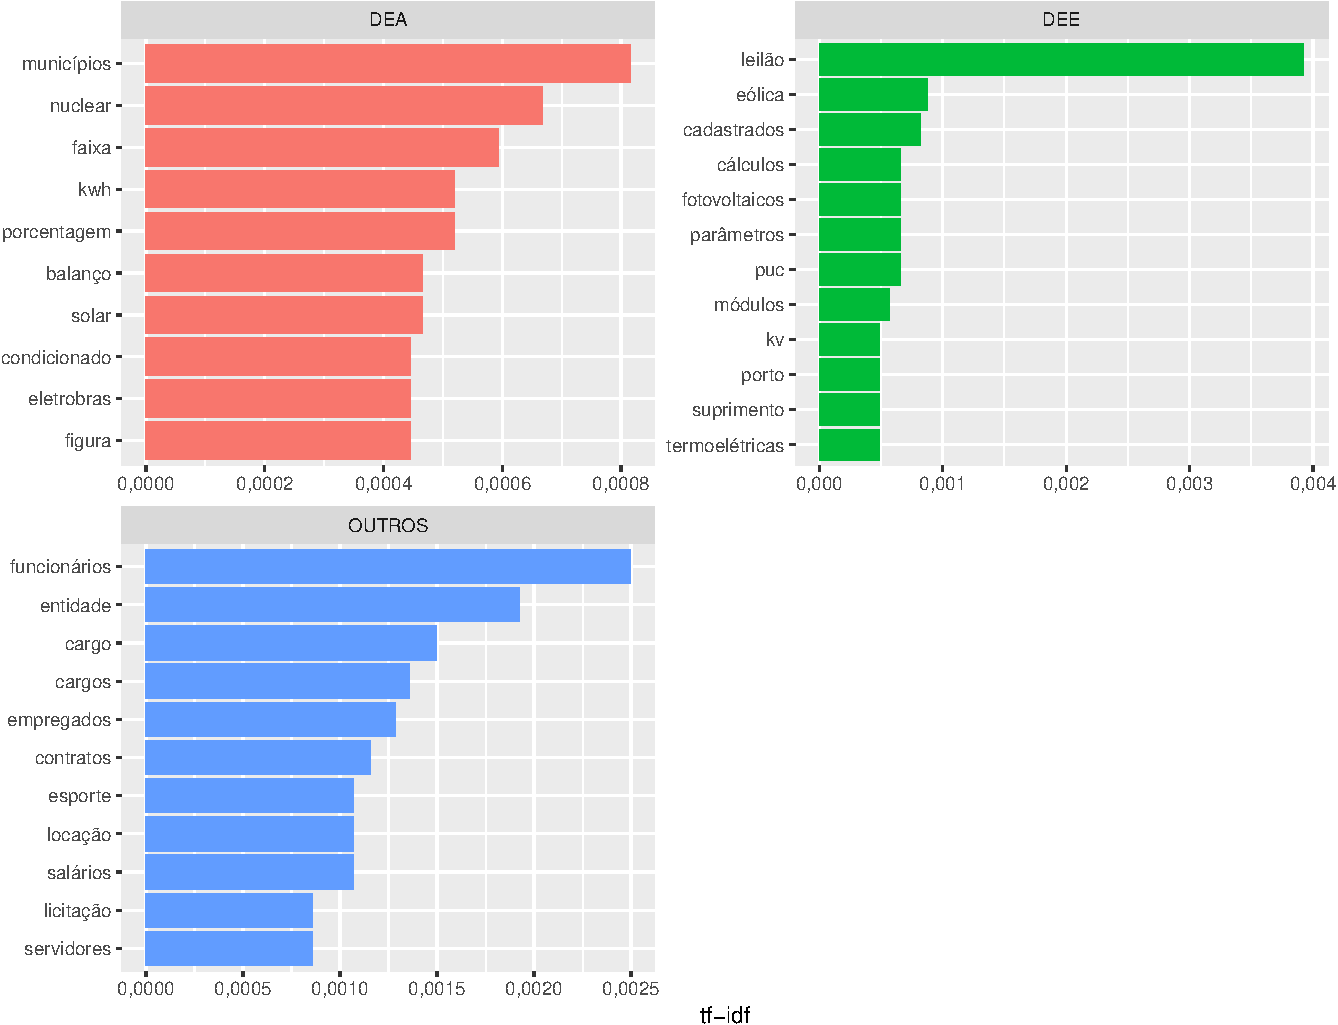
\includegraphics{markdown_v40_test_files/figure-latex/02_freq_palavras_dir-1.pdf}

\begin{Shaded}
\begin{Highlighting}[]
\CommentTok{#dev.off()}
\end{Highlighting}
\end{Shaded}

\paragraph{Filtrando um pedaço de
texto}\label{filtrando-um-pedaco-de-texto}

\begin{Shaded}
\begin{Highlighting}[]
\NormalTok{DB }\OperatorTok
\StringTok{  }\KeywordTok{filter}\NormalTok{(}\KeywordTok{str_detect}\NormalTok{(DESCRI_PEDIDO, }\StringTok{"r0"}\NormalTok{)) }\OperatorTok
\StringTok{  }\KeywordTok{select}\NormalTok{(DESCRI_PEDIDO) }\OperatorTok
\StringTok{  }\KeywordTok{head}\NormalTok{()}
\end{Highlighting}
\end{Shaded}

\begin{verbatim}
## # A tibble: 6 x 1
##   DESCRI_PEDIDO                                                            
##   <chr>                                                                    
## 1 "Prezados,\n\nSolicitamos que o deck do Newave 22.6 utilizado para Revis~
## 2 Gostaria de ter acesso à Nota Técnica EPE-DEE-RE-097/2016-r0, pois não a~
## 3 "Solicitamos para nossa análise cópias dos relatórios nºs EPE-DEE-RE-147~
## 4 Cópia do documento EPE-DEE-RE-083/2010-r0, “Estudo de Integração das Usi~
## 5 Solicito cópia da Nota Técnica EPE-DEE-RE-097/2016-r0                    
## 6 "Bom dia, por gentileza gostaria ter acesso ao parecer técnico EPE-DEE-P~
\end{verbatim}

Uma limpeza removendo palavras sem significado semântico (\textbf{stop
words}) pode auxiliar o algoritmo a retornar palavras ainda mais
acertivas, bem como o tratamento de \textbf{stemming}, abordados a
seguir.

\subsubsection{Stemming}\label{stemming}

Podemos diminuir redundâncias por parte do algoritmo ensinando-o a
compreender palavras que podem estar escritas de forma diferente mas que
em significado semântico são semelhantes. Para isso, analisamos o
radical de palavras com um mesmo prefixo mas com sufixos diferentes seja
por quisistos como gênero ou plural.

Exemplos:

leilão \(\propto\) leilões estado \(\propto\) estados região \(\propto\)
regiões

Usando o pacote \texttt{ptstem}

\begin{Shaded}
\begin{Highlighting}[]
\KeywordTok{library}\NormalTok{(ptstem)}
\NormalTok{stemming1 =}\StringTok{ }\KeywordTok{ptstem}\NormalTok{(DB}\OperatorTok{$}\NormalTok{DESCRI_PEDIDO)}
\end{Highlighting}
\end{Shaded}

\begin{itemize}
\tightlist
\item
  Frequência de palavras por diretoria do stemming 1
\end{itemize}

\begin{Shaded}
\begin{Highlighting}[]
\NormalTok{diretoria_palavras_stem1 <-}\StringTok{ }\NormalTok{DB }\OperatorTok
\StringTok{  }\KeywordTok{mutate}\NormalTok{(}\DataTypeTok{DESCRI_PEDIDO =}\NormalTok{ stemming1) }\OperatorTok
\StringTok{  }\KeywordTok{unnest_tokens}\NormalTok{(palavra, DESCRI_PEDIDO) }\OperatorTok
\StringTok{  }\KeywordTok{count}\NormalTok{(palavra, }\DataTypeTok{sort =} \OtherTok{TRUE}\NormalTok{) }\OperatorTok
\StringTok{  }\KeywordTok{ungroup}\NormalTok{()}
\end{Highlighting}
\end{Shaded}

\begin{Shaded}
\begin{Highlighting}[]
\KeywordTok{cat}\NormalTok{(}\KeywordTok{paste0}\NormalTok{(}\StringTok{"Utilizando o algoritmo de stemming do pacote 'ptstem' o número de palavras chaves sem stemming reduziu de "}\NormalTok{, }\KeywordTok{dim}\NormalTok{(diretoria_palavras)[}\DecValTok{1}\NormalTok{], }\StringTok{" para "}\NormalTok{, }\KeywordTok{dim}\NormalTok{(diretoria_palavras_stem1)[}\DecValTok{1}\NormalTok{], }\StringTok{", após stemming. Uma redução de "}\NormalTok{,}\KeywordTok{round}\NormalTok{(}\DecValTok{100}\OperatorTok{-}\KeywordTok{dim}\NormalTok{(diretoria_palavras_stem1)[}\DecValTok{1}\NormalTok{]}\OperatorTok{*}\DecValTok{100}\OperatorTok{/}\KeywordTok{dim}\NormalTok{(diretoria_palavras)[}\DecValTok{1}\NormalTok{],}\DecValTok{0}\NormalTok{),}\StringTok{"%."}\NormalTok{))}
\end{Highlighting}
\end{Shaded}

\begin{verbatim}
## Utilizando o algoritmo de stemming do pacote 'ptstem' o número de palavras chaves sem stemming reduziu de 8501 para 4048, após stemming. Uma redução de 52%.
\end{verbatim}

Usando o pacote \texttt{rslp}

\begin{Shaded}
\begin{Highlighting}[]
\KeywordTok{library}\NormalTok{(rslp)}
\NormalTok{stemming2 =}\StringTok{ }\KeywordTok{rslp}\NormalTok{(DB}\OperatorTok{$}\NormalTok{DESCRI_PEDIDO)}
\end{Highlighting}
\end{Shaded}

\begin{itemize}
\tightlist
\item
  Frequência de palavras por diretoria do stemming 2
\end{itemize}

\begin{Shaded}
\begin{Highlighting}[]
\NormalTok{diretoria_palavras_stem2 <-}\StringTok{ }\NormalTok{DB }\OperatorTok
\StringTok{  }\KeywordTok{mutate}\NormalTok{(}\DataTypeTok{DESCRI_PEDIDO =}\NormalTok{ stemming2) }\OperatorTok
\StringTok{  }\KeywordTok{unnest_tokens}\NormalTok{(palavra, DESCRI_PEDIDO) }\OperatorTok
\StringTok{  }\KeywordTok{count}\NormalTok{(palavra, }\DataTypeTok{sort =} \OtherTok{TRUE}\NormalTok{) }\OperatorTok
\StringTok{  }\KeywordTok{ungroup}\NormalTok{()}
\end{Highlighting}
\end{Shaded}

\begin{Shaded}
\begin{Highlighting}[]
\KeywordTok{cat}\NormalTok{(}\KeywordTok{paste0}\NormalTok{(}\StringTok{"Utilizando o algoritmo de stemming do pacote 'rslp' o número de palavras chaves sem stemming reduziu de "}\NormalTok{, }\KeywordTok{dim}\NormalTok{(diretoria_palavras)[}\DecValTok{1}\NormalTok{], }\StringTok{" para "}\NormalTok{, }\KeywordTok{dim}\NormalTok{(diretoria_palavras_stem2)[}\DecValTok{1}\NormalTok{], }\StringTok{", após stemming. Uma redução de "}\NormalTok{, }\KeywordTok{round}\NormalTok{(}\DecValTok{100}\OperatorTok{-}\KeywordTok{dim}\NormalTok{(diretoria_palavras_stem2)[}\DecValTok{1}\NormalTok{]}\OperatorTok{*}\DecValTok{100}\OperatorTok{/}\KeywordTok{dim}\NormalTok{(diretoria_palavras)[}\DecValTok{1}\NormalTok{],}\DecValTok{0}\NormalTok{),}\StringTok{"%."}\NormalTok{))}
\end{Highlighting}
\end{Shaded}

\begin{verbatim}
## Utilizando o algoritmo de stemming do pacote 'rslp' o número de palavras chaves sem stemming reduziu de 8501 para 5626, após stemming. Uma redução de 34%.
\end{verbatim}

Uma redução considerável no número de termos ocorreu ao usar o algoritmo
\texttt{ptstem}, cerca de \(33\%\) de redução de termos versus \(7\%\)
utilziando o algoritmo \texttt{rslp}, ou seja, o algoritmo ptstem foi
mais eficiente na tarefa de agrupar os semelhantes (termos únicos).

Vale ressaltar, tabmbém, o tempo de processamento que ambos os
algoritmos requerem.

\begin{Shaded}
\begin{Highlighting}[]
\NormalTok{temp_stem1 =}\StringTok{ }\KeywordTok{proc.time}\NormalTok{()}
\NormalTok{teste0 =}\StringTok{ }\KeywordTok{ptstem}\NormalTok{(DB}\OperatorTok{$}\NormalTok{DESCRI_PEDIDO)}
\NormalTok{tempo_stem1 =}\StringTok{ }\KeywordTok{proc.time}\NormalTok{() }\OperatorTok{-}\StringTok{ }\NormalTok{temp_stem1}
\KeywordTok{remove}\NormalTok{(teste0)}
\end{Highlighting}
\end{Shaded}

\begin{Shaded}
\begin{Highlighting}[]
\NormalTok{temp_stem2 =}\StringTok{ }\KeywordTok{proc.time}\NormalTok{()}
\NormalTok{teste00 =}\StringTok{ }\KeywordTok{rslp}\NormalTok{(DB}\OperatorTok{$}\NormalTok{DESCRI_PEDIDO)}
\NormalTok{tempo_stem2 =}\StringTok{ }\KeywordTok{proc.time}\NormalTok{() }\OperatorTok{-}\StringTok{ }\NormalTok{temp_stem2}
\KeywordTok{remove}\NormalTok{(teste00)}
\end{Highlighting}
\end{Shaded}

O tempo decorrido para processamento do algoritmo do \texttt{ptstem} foi
de aproximadamente 12,5 segundos versus 0,9 segundo decorrido para o
processamento do algoritmo do \texttt{rslp}. Logo, o \texttt{rslp} é
quase 14 vezes mais eficiente em termos de tempo de processamento. Além
disso, o \texttt{rslp} remove acentuações e caracteres como ``ç''. Isso
irá nos ajudar mais a frente quando utilizarmos os principais termos
como variáveis binárias e preditoras do modelo de classificação.

Entretanto, o algoritmo mais lento, \texttt{ptstem}, foi mais
interessante em termos de redução do número de termos únicos, cerca de
26\% menos termos únicos em relação ao outro algoritmo. Além disso, por
se tratar de uma base de dados relativamente pequena, 625 pedidos, e
pouco mais de 4 mil termos únicos em todo o conjunto de texto, além
disso vamos utilizar de um alto poder de processamento da máquina no
referido estudo. Optamos, portanto, por utilizar ambos algoritmos.
Vamos, primeiro, aplicar o removedor de sufixos da lingua portuguesa
\texttt{rslp} seguido do \texttt{ptstem}.

Cria, antes, uma variáveil DESCRI\_PEDIDO1 que repete os passos feitos
aos termos quanto ao stemming so que no texto fonte.

\begin{Shaded}
\begin{Highlighting}[]
\NormalTok{### CARACTERES}
\NormalTok{DB}\OperatorTok{$}\NormalTok{DESCRI_PEDIDO1 =}\StringTok{ }\NormalTok{DB}\OperatorTok{$}\NormalTok{DESCRI_PEDIDO}
\NormalTok{DB}\OperatorTok{$}\NormalTok{DESCRI_PEDIDO1 =}\StringTok{ }\KeywordTok{gsub}\NormalTok{(}\StringTok{"-"}\NormalTok{,}\StringTok{""}\NormalTok{,DB}\OperatorTok{$}\NormalTok{DESCRI_PEDIDO1)}
\NormalTok{DB}\OperatorTok{$}\NormalTok{DESCRI_PEDIDO1 =}\StringTok{ }\KeywordTok{gsub}\NormalTok{(}\StringTok{"[:.:]"}\NormalTok{,}\StringTok{""}\NormalTok{,DB}\OperatorTok{$}\NormalTok{DESCRI_PEDIDO1)}
\NormalTok{DB}\OperatorTok{$}\NormalTok{DESCRI_PEDIDO1 =}\StringTok{ }\KeywordTok{gsub}\NormalTok{(}\StringTok{"[:,:]"}\NormalTok{,}\StringTok{""}\NormalTok{,DB}\OperatorTok{$}\NormalTok{DESCRI_PEDIDO1)}
\NormalTok{DB}\OperatorTok{$}\NormalTok{DESCRI_PEDIDO1 =}\StringTok{ }\KeywordTok{gsub}\NormalTok{(}\StringTok{"[:':]"}\NormalTok{,}\StringTok{""}\NormalTok{,DB}\OperatorTok{$}\NormalTok{DESCRI_PEDIDO1)}
\NormalTok{DB}\OperatorTok{$}\NormalTok{DESCRI_PEDIDO1 =}\StringTok{ }\KeywordTok{gsub}\NormalTok{(}\StringTok{"[:!:]"}\NormalTok{,}\StringTok{""}\NormalTok{,DB}\OperatorTok{$}\NormalTok{DESCRI_PEDIDO1)}
\NormalTok{DB}\OperatorTok{$}\NormalTok{DESCRI_PEDIDO1 =}\StringTok{ }\KeywordTok{gsub}\NormalTok{(}\StringTok{"[:?:]"}\NormalTok{,}\StringTok{""}\NormalTok{,DB}\OperatorTok{$}\NormalTok{DESCRI_PEDIDO1)}
\NormalTok{DB}\OperatorTok{$}\NormalTok{DESCRI_PEDIDO1 =}\StringTok{ }\KeywordTok{gsub}\NormalTok{(}\StringTok{"[:-:]"}\NormalTok{,}\StringTok{""}\NormalTok{,DB}\OperatorTok{$}\NormalTok{DESCRI_PEDIDO1)}
\NormalTok{DB}\OperatorTok{$}\NormalTok{DESCRI_PEDIDO1 =}\StringTok{ }\KeywordTok{gsub}\NormalTok{(}\StringTok{"[:__:]"}\NormalTok{,}\StringTok{""}\NormalTok{,DB}\OperatorTok{$}\NormalTok{DESCRI_PEDIDO1)}
\NormalTok{DB}\OperatorTok{$}\NormalTok{DESCRI_PEDIDO1 =}\StringTok{ }\KeywordTok{gsub}\NormalTok{(}\StringTok{"[:;:]"}\NormalTok{,}\StringTok{""}\NormalTok{,DB}\OperatorTok{$}\NormalTok{DESCRI_PEDIDO1)}
\NormalTok{DB}\OperatorTok{$}\NormalTok{DESCRI_PEDIDO1 =}\StringTok{ }\KeywordTok{gsub}\NormalTok{(}\StringTok{"[:/:]"}\NormalTok{,}\StringTok{""}\NormalTok{,DB}\OperatorTok{$}\NormalTok{DESCRI_PEDIDO1)}
\NormalTok{DB}\OperatorTok{$}\NormalTok{DESCRI_PEDIDO1 =}\StringTok{ }\KeywordTok{gsub}\NormalTok{(}\StringTok{"[:(:]"}\NormalTok{,}\StringTok{""}\NormalTok{,DB}\OperatorTok{$}\NormalTok{DESCRI_PEDIDO1)}
\NormalTok{DB}\OperatorTok{$}\NormalTok{DESCRI_PEDIDO1 =}\StringTok{ }\KeywordTok{gsub}\NormalTok{(}\StringTok{"[:):]"}\NormalTok{,}\StringTok{""}\NormalTok{,DB}\OperatorTok{$}\NormalTok{DESCRI_PEDIDO1)}
\NormalTok{DB}\OperatorTok{$}\NormalTok{DESCRI_PEDIDO1 =}\StringTok{ }\KeywordTok{gsub}\NormalTok{(}\StringTok{"[:%:]"}\NormalTok{,}\StringTok{""}\NormalTok{,DB}\OperatorTok{$}\NormalTok{DESCRI_PEDIDO1)}
\NormalTok{DB}\OperatorTok{$}\NormalTok{DESCRI_PEDIDO1 =}\StringTok{ }\KeywordTok{gsub}\NormalTok{(}\StringTok{"[:º:]"}\NormalTok{,}\StringTok{""}\NormalTok{,DB}\OperatorTok{$}\NormalTok{DESCRI_PEDIDO1)}
\NormalTok{DB}\OperatorTok{$}\NormalTok{DESCRI_PEDIDO1 =}\StringTok{ }\KeywordTok{gsub}\NormalTok{(}\StringTok{"[:°:]"}\NormalTok{,}\StringTok{""}\NormalTok{,DB}\OperatorTok{$}\NormalTok{DESCRI_PEDIDO1)}
\NormalTok{DB}\OperatorTok{$}\NormalTok{DESCRI_PEDIDO1 =}\StringTok{ }\KeywordTok{gsub}\NormalTok{(}\StringTok{"[:ª:]"}\NormalTok{,}\StringTok{""}\NormalTok{,DB}\OperatorTok{$}\NormalTok{DESCRI_PEDIDO1)}
\NormalTok{DB}\OperatorTok{$}\NormalTok{DESCRI_PEDIDO1 =}\StringTok{ }\KeywordTok{gsub}\NormalTok{(}\StringTok{"}\CharTok{\textbackslash{}\textbackslash{}}\StringTok{d+"}\NormalTok{,}\StringTok{""}\NormalTok{,DB}\OperatorTok{$}\NormalTok{DESCRI_PEDIDO1)}
\NormalTok{DB}\OperatorTok{$}\NormalTok{DESCRI_PEDIDO1 =}\StringTok{ }\KeywordTok{gsub}\NormalTok{(}\StringTok{"[0-9]"}\NormalTok{,}\StringTok{""}\NormalTok{,DB}\OperatorTok{$}\NormalTok{DESCRI_PEDIDO1)}
\NormalTok{DB}\OperatorTok{$}\NormalTok{DESCRI_PEDIDO1 =}\StringTok{ }\KeywordTok{gsub}\NormalTok{(}\StringTok{"[:}\CharTok{\textbackslash{}n\textbackslash{}t}\StringTok{:]"}\NormalTok{,}\StringTok{" "}\NormalTok{,DB}\OperatorTok{$}\NormalTok{DESCRI_PEDIDO1)}
\NormalTok{DB}\OperatorTok{$}\NormalTok{DESCRI_PEDIDO1 =}\StringTok{ }\KeywordTok{gsub}\NormalTok{(}\StringTok{"[:}\CharTok{\textbackslash{}t}\StringTok{:]"}\NormalTok{,}\StringTok{""}\NormalTok{,DB}\OperatorTok{$}\NormalTok{DESCRI_PEDIDO1)}
\NormalTok{DB}\OperatorTok{$}\NormalTok{DESCRI_PEDIDO1 =}\StringTok{ }\KeywordTok{gsub}\NormalTok{(}\StringTok{"[:}\CharTok{\textbackslash{}n}\StringTok{:]"}\NormalTok{,}\StringTok{""}\NormalTok{,DB}\OperatorTok{$}\NormalTok{DESCRI_PEDIDO1)}
\NormalTok{DB}\OperatorTok{$}\NormalTok{DESCRI_PEDIDO1 =}\StringTok{ }\KeywordTok{gsub}\NormalTok{(}\StringTok{"}\CharTok{\textbackslash{}\textbackslash{}}\StringTok{s+"}\NormalTok{,}\StringTok{" "}\NormalTok{,DB}\OperatorTok{$}\NormalTok{DESCRI_PEDIDO1)}
\NormalTok{DB}\OperatorTok{$}\NormalTok{DESCRI_PEDIDO1 =}\StringTok{ }\KeywordTok{gsub}\NormalTok{(}\StringTok{"}\CharTok{\textbackslash{}"}\StringTok{"}\NormalTok{,}\StringTok{""}\NormalTok{,DB}\OperatorTok{$}\NormalTok{DESCRI_PEDIDO1)}

\NormalTok{### STEMMINGS}
\NormalTok{DB}\OperatorTok{$}\NormalTok{DESCRI_PEDIDO1 =}\StringTok{ }\KeywordTok{ptstem}\NormalTok{(}\KeywordTok{rslp}\NormalTok{(DB}\OperatorTok{$}\NormalTok{DESCRI_PEDIDO1), }\DataTypeTok{algorithm =} \StringTok{"hunspell"}\NormalTok{, }
                           \DataTypeTok{complete =} \OtherTok{TRUE}\NormalTok{)}
\NormalTok{DB}\OperatorTok{$}\NormalTok{DESCRI_PEDIDO1 =}\StringTok{ }\KeywordTok{rslp}\NormalTok{(}\KeywordTok{ptstem}\NormalTok{(DB}\OperatorTok{$}\NormalTok{DESCRI_PEDIDO1))}
\NormalTok{DB}\OperatorTok{$}\NormalTok{DESCRI_PEDIDO1 =}\StringTok{ }\KeywordTok{gsub}\NormalTok{(}\StringTok{"}\CharTok{\textbackslash{}\textbackslash{}}\StringTok{s+"}\NormalTok{,}\StringTok{" "}\NormalTok{,DB}\OperatorTok{$}\NormalTok{DESCRI_PEDIDO1)}


\NormalTok{### PALAVRAS}
\NormalTok{DB}\OperatorTok{$}\NormalTok{DESCRI_PEDIDO1 =}\KeywordTok{gsub}\NormalTok{(}\StringTok{"}\CharTok{\textbackslash{}\textbackslash{}}\StringTok{b(Leiloes)"}\NormalTok{, }\StringTok{"leilao"}\NormalTok{, DB}\OperatorTok{$}\NormalTok{DESCRI_PEDIDO1)}
\NormalTok{DB}\OperatorTok{$}\NormalTok{DESCRI_PEDIDO1 =}\KeywordTok{gsub}\NormalTok{(}\StringTok{"}\CharTok{\textbackslash{}\textbackslash{}}\StringTok{b(Leiloar)"}\NormalTok{, }\StringTok{"leilao"}\NormalTok{, DB}\OperatorTok{$}\NormalTok{DESCRI_PEDIDO1)}
\NormalTok{DB}\OperatorTok{$}\NormalTok{DESCRI_PEDIDO1 =}\KeywordTok{gsub}\NormalTok{(}\StringTok{"}\CharTok{\textbackslash{}\textbackslash{}}\StringTok{b(leiloes)"}\NormalTok{, }\StringTok{"leilao"}\NormalTok{, DB}\OperatorTok{$}\NormalTok{DESCRI_PEDIDO1)}
\NormalTok{DB}\OperatorTok{$}\NormalTok{DESCRI_PEDIDO1 =}\KeywordTok{gsub}\NormalTok{(}\StringTok{"}\CharTok{\textbackslash{}\textbackslash{}}\StringTok{b(leiloar)"}\NormalTok{, }\StringTok{"leilao"}\NormalTok{, DB}\OperatorTok{$}\NormalTok{DESCRI_PEDIDO1)}
\NormalTok{DB}\OperatorTok{$}\NormalTok{DESCRI_PEDIDO1 =}\KeywordTok{gsub}\NormalTok{(}\StringTok{"}\CharTok{\textbackslash{}\textbackslash{}}\StringTok{b(leiloes)"}\NormalTok{, }\StringTok{"leilao"}\NormalTok{, DB}\OperatorTok{$}\NormalTok{DESCRI_PEDIDO1)}
\NormalTok{DB}\OperatorTok{$}\NormalTok{DESCRI_PEDIDO1 =}\KeywordTok{gsub}\NormalTok{(}\StringTok{"}\CharTok{\textbackslash{}\textbackslash{}}\StringTok{b(Energetica)"}\NormalTok{, }\StringTok{"eletrica"}\NormalTok{, DB}\OperatorTok{$}\NormalTok{DESCRI_PEDIDO1)}
\NormalTok{DB}\OperatorTok{$}\NormalTok{DESCRI_PEDIDO1 =}\KeywordTok{gsub}\NormalTok{(}\StringTok{"}\CharTok{\textbackslash{}\textbackslash{}}\StringTok{b(energetica)"}\NormalTok{, }\StringTok{"eletrica"}\NormalTok{, DB}\OperatorTok{$}\NormalTok{DESCRI_PEDIDO1)}
\NormalTok{DB}\OperatorTok{$}\NormalTok{DESCRI_PEDIDO1 =}\KeywordTok{gsub}\NormalTok{(}\StringTok{"}\CharTok{\textbackslash{}\textbackslash{}}\StringTok{b(Eletricas)"}\NormalTok{, }\StringTok{"eletrica"}\NormalTok{, DB}\OperatorTok{$}\NormalTok{DESCRI_PEDIDO1)}
\NormalTok{DB}\OperatorTok{$}\NormalTok{DESCRI_PEDIDO1 =}\KeywordTok{gsub}\NormalTok{(}\StringTok{"}\CharTok{\textbackslash{}\textbackslash{}}\StringTok{b(eletricas)"}\NormalTok{, }\StringTok{"eletrica"}\NormalTok{, DB}\OperatorTok{$}\NormalTok{DESCRI_PEDIDO1)}
\NormalTok{DB}\OperatorTok{$}\NormalTok{DESCRI_PEDIDO1 =}\KeywordTok{gsub}\NormalTok{(}\StringTok{"}\CharTok{\textbackslash{}\textbackslash{}}\StringTok{b(Eletricos)"}\NormalTok{, }\StringTok{"eletrica"}\NormalTok{, DB}\OperatorTok{$}\NormalTok{DESCRI_PEDIDO1)}
\NormalTok{DB}\OperatorTok{$}\NormalTok{DESCRI_PEDIDO1 =}\KeywordTok{gsub}\NormalTok{(}\StringTok{"}\CharTok{\textbackslash{}\textbackslash{}}\StringTok{b(eletricos)"}\NormalTok{, }\StringTok{"eletrica"}\NormalTok{, DB}\OperatorTok{$}\NormalTok{DESCRI_PEDIDO1)}
\NormalTok{DB}\OperatorTok{$}\NormalTok{DESCRI_PEDIDO1 =}\KeywordTok{gsub}\NormalTok{(}\StringTok{"}\CharTok{\textbackslash{}\textbackslash{}}\StringTok{b(Eletrico)"}\NormalTok{, }\StringTok{"eletrica"}\NormalTok{, DB}\OperatorTok{$}\NormalTok{DESCRI_PEDIDO1)}
\NormalTok{DB}\OperatorTok{$}\NormalTok{DESCRI_PEDIDO1 =}\KeywordTok{gsub}\NormalTok{(}\StringTok{"}\CharTok{\textbackslash{}\textbackslash{}}\StringTok{b(eletrico)"}\NormalTok{, }\StringTok{"eletrica"}\NormalTok{, DB}\OperatorTok{$}\NormalTok{DESCRI_PEDIDO1)}
\NormalTok{DB}\OperatorTok{$}\NormalTok{DESCRI_PEDIDO1 =}\KeywordTok{gsub}\NormalTok{(}\StringTok{"}\CharTok{\textbackslash{}\textbackslash{}}\StringTok{b(Eletricidade)"}\NormalTok{, }\StringTok{"eletrica"}\NormalTok{, DB}\OperatorTok{$}\NormalTok{DESCRI_PEDIDO1)}
\NormalTok{DB}\OperatorTok{$}\NormalTok{DESCRI_PEDIDO1 =}\KeywordTok{gsub}\NormalTok{(}\StringTok{"}\CharTok{\textbackslash{}\textbackslash{}}\StringTok{b(eletricidade)"}\NormalTok{, }\StringTok{"eletrica"}\NormalTok{, DB}\OperatorTok{$}\NormalTok{DESCRI_PEDIDO1)}
\NormalTok{DB}\OperatorTok{$}\NormalTok{DESCRI_PEDIDO1 =}\KeywordTok{gsub}\NormalTok{(}\StringTok{"}\CharTok{\textbackslash{}\textbackslash{}}\StringTok{b(Termoeletricas)"}\NormalTok{, }\StringTok{"termoeletrica"}\NormalTok{, DB}\OperatorTok{$}\NormalTok{DESCRI_PEDIDO1)}
\NormalTok{DB}\OperatorTok{$}\NormalTok{DESCRI_PEDIDO1 =}\KeywordTok{gsub}\NormalTok{(}\StringTok{"}\CharTok{\textbackslash{}\textbackslash{}}\StringTok{b(termoeletricas)"}\NormalTok{, }\StringTok{"termoeletrica"}\NormalTok{, DB}\OperatorTok{$}\NormalTok{DESCRI_PEDIDO1)}
\NormalTok{DB}\OperatorTok{$}\NormalTok{DESCRI_PEDIDO1 =}\KeywordTok{gsub}\NormalTok{(}\StringTok{"}\CharTok{\textbackslash{}\textbackslash{}}\StringTok{b(Termeletrica)"}\NormalTok{, }\StringTok{"termoeletrica"}\NormalTok{, DB}\OperatorTok{$}\NormalTok{DESCRI_PEDIDO1)}
\NormalTok{DB}\OperatorTok{$}\NormalTok{DESCRI_PEDIDO1 =}\KeywordTok{gsub}\NormalTok{(}\StringTok{"}\CharTok{\textbackslash{}\textbackslash{}}\StringTok{b(termeletrica)"}\NormalTok{, }\StringTok{"termoeletrica"}\NormalTok{, DB}\OperatorTok{$}\NormalTok{DESCRI_PEDIDO1)}
\NormalTok{DB}\OperatorTok{$}\NormalTok{DESCRI_PEDIDO1 =}\KeywordTok{gsub}\NormalTok{(}\StringTok{"}\CharTok{\textbackslash{}\textbackslash{}}\StringTok{b(Termeletricas)"}\NormalTok{, }\StringTok{"termoeletrica"}\NormalTok{, DB}\OperatorTok{$}\NormalTok{DESCRI_PEDIDO1)}
\NormalTok{DB}\OperatorTok{$}\NormalTok{DESCRI_PEDIDO1 =}\KeywordTok{gsub}\NormalTok{(}\StringTok{"}\CharTok{\textbackslash{}\textbackslash{}}\StringTok{b(termeletricas)"}\NormalTok{, }\StringTok{"termoeletrica"}\NormalTok{, DB}\OperatorTok{$}\NormalTok{DESCRI_PEDIDO1)}
\NormalTok{DB}\OperatorTok{$}\NormalTok{DESCRI_PEDIDO1 =}\KeywordTok{gsub}\NormalTok{(}\StringTok{"}\CharTok{\textbackslash{}\textbackslash{}}\StringTok{b(Hidreletricas)"}\NormalTok{, }\StringTok{"hidreletrica"}\NormalTok{, DB}\OperatorTok{$}\NormalTok{DESCRI_PEDIDO1)}
\NormalTok{DB}\OperatorTok{$}\NormalTok{DESCRI_PEDIDO1 =}\KeywordTok{gsub}\NormalTok{(}\StringTok{"}\CharTok{\textbackslash{}\textbackslash{}}\StringTok{b(hidreletricas)"}\NormalTok{, }\StringTok{"hidreletrica"}\NormalTok{, DB}\OperatorTok{$}\NormalTok{DESCRI_PEDIDO1)}
\NormalTok{DB}\OperatorTok{$}\NormalTok{DESCRI_PEDIDO1 =}\KeywordTok{gsub}\NormalTok{(}\StringTok{"}\CharTok{\textbackslash{}\textbackslash{}}\StringTok{b(Hidroeletricas)"}\NormalTok{, }\StringTok{"hidreletrica"}\NormalTok{, DB}\OperatorTok{$}\NormalTok{DESCRI_PEDIDO1)}
\NormalTok{DB}\OperatorTok{$}\NormalTok{DESCRI_PEDIDO1 =}\KeywordTok{gsub}\NormalTok{(}\StringTok{"}\CharTok{\textbackslash{}\textbackslash{}}\StringTok{b(hidroeletricas)"}\NormalTok{, }\StringTok{"hidreletrica"}\NormalTok{, DB}\OperatorTok{$}\NormalTok{DESCRI_PEDIDO1)}
\NormalTok{DB}\OperatorTok{$}\NormalTok{DESCRI_PEDIDO1 =}\KeywordTok{gsub}\NormalTok{(}\StringTok{"}\CharTok{\textbackslash{}\textbackslash{}}\StringTok{b(Hidroeletricos)"}\NormalTok{, }\StringTok{"hidreletrica"}\NormalTok{, DB}\OperatorTok{$}\NormalTok{DESCRI_PEDIDO1)}
\NormalTok{DB}\OperatorTok{$}\NormalTok{DESCRI_PEDIDO1 =}\KeywordTok{gsub}\NormalTok{(}\StringTok{"}\CharTok{\textbackslash{}\textbackslash{}}\StringTok{b(hidroeletricos)"}\NormalTok{, }\StringTok{"hidreletrica"}\NormalTok{, DB}\OperatorTok{$}\NormalTok{DESCRI_PEDIDO1)}
\NormalTok{DB}\OperatorTok{$}\NormalTok{DESCRI_PEDIDO1 =}\KeywordTok{gsub}\NormalTok{(}\StringTok{"}\CharTok{\textbackslash{}\textbackslash{}}\StringTok{b(Hidroeletrica)"}\NormalTok{, }\StringTok{"hidreletrica"}\NormalTok{, DB}\OperatorTok{$}\NormalTok{DESCRI_PEDIDO1)}
\NormalTok{DB}\OperatorTok{$}\NormalTok{DESCRI_PEDIDO1 =}\KeywordTok{gsub}\NormalTok{(}\StringTok{"}\CharTok{\textbackslash{}\textbackslash{}}\StringTok{b(hidroeletrica)"}\NormalTok{, }\StringTok{"hidreletrica"}\NormalTok{, DB}\OperatorTok{$}\NormalTok{DESCRI_PEDIDO1)}
\NormalTok{DB}\OperatorTok{$}\NormalTok{DESCRI_PEDIDO1 =}\KeywordTok{gsub}\NormalTok{(}\StringTok{"}\CharTok{\textbackslash{}\textbackslash{}}\StringTok{b(Administracao)"}\NormalTok{, }\StringTok{"administracao"}\NormalTok{, DB}\OperatorTok{$}\NormalTok{DESCRI_PEDIDO1)}
\NormalTok{DB}\OperatorTok{$}\NormalTok{DESCRI_PEDIDO1 =}\KeywordTok{gsub}\NormalTok{(}\StringTok{"}\CharTok{\textbackslash{}\textbackslash{}}\StringTok{b(administracao)"}\NormalTok{, }\StringTok{"administracao"}\NormalTok{, DB}\OperatorTok{$}\NormalTok{DESCRI_PEDIDO1)}
\NormalTok{DB}\OperatorTok{$}\NormalTok{DESCRI_PEDIDO1 =}\KeywordTok{gsub}\NormalTok{(}\StringTok{"}\CharTok{\textbackslash{}\textbackslash{}}\StringTok{b(Administrativo)"}\NormalTok{, }\StringTok{"administracao"}\NormalTok{, DB}\OperatorTok{$}\NormalTok{DESCRI_PEDIDO1)}
\NormalTok{DB}\OperatorTok{$}\NormalTok{DESCRI_PEDIDO1 =}\KeywordTok{gsub}\NormalTok{(}\StringTok{"}\CharTok{\textbackslash{}\textbackslash{}}\StringTok{b(administrativo)"}\NormalTok{, }\StringTok{"administracao"}\NormalTok{, DB}\OperatorTok{$}\NormalTok{DESCRI_PEDIDO1)}
\NormalTok{DB}\OperatorTok{$}\NormalTok{DESCRI_PEDIDO1 =}\KeywordTok{gsub}\NormalTok{(}\StringTok{"}\CharTok{\textbackslash{}\textbackslash{}}\StringTok{b(Administrativos)"}\NormalTok{, }\StringTok{"administracao"}\NormalTok{, DB}\OperatorTok{$}\NormalTok{DESCRI_PEDIDO1)}
\NormalTok{DB}\OperatorTok{$}\NormalTok{DESCRI_PEDIDO1 =}\KeywordTok{gsub}\NormalTok{(}\StringTok{"}\CharTok{\textbackslash{}\textbackslash{}}\StringTok{b(administrativos)"}\NormalTok{, }\StringTok{"administracao"}\NormalTok{, DB}\OperatorTok{$}\NormalTok{DESCRI_PEDIDO1)}
\NormalTok{DB}\OperatorTok{$}\NormalTok{DESCRI_PEDIDO1 =}\KeywordTok{gsub}\NormalTok{(}\StringTok{"}\CharTok{\textbackslash{}\textbackslash{}}\StringTok{b(Administrativa)"}\NormalTok{, }\StringTok{"administracao"}\NormalTok{, DB}\OperatorTok{$}\NormalTok{DESCRI_PEDIDO1)}
\NormalTok{DB}\OperatorTok{$}\NormalTok{DESCRI_PEDIDO1 =}\KeywordTok{gsub}\NormalTok{(}\StringTok{"}\CharTok{\textbackslash{}\textbackslash{}}\StringTok{b(administrativa)"}\NormalTok{, }\StringTok{"administracao"}\NormalTok{, DB}\OperatorTok{$}\NormalTok{DESCRI_PEDIDO1)}
\NormalTok{DB}\OperatorTok{$}\NormalTok{DESCRI_PEDIDO1 =}\KeywordTok{gsub}\NormalTok{(}\StringTok{"}\CharTok{\textbackslash{}\textbackslash{}}\StringTok{b(Administrativas)"}\NormalTok{, }\StringTok{"administracao"}\NormalTok{, DB}\OperatorTok{$}\NormalTok{DESCRI_PEDIDO1)}
\NormalTok{DB}\OperatorTok{$}\NormalTok{DESCRI_PEDIDO1 =}\KeywordTok{gsub}\NormalTok{(}\StringTok{"}\CharTok{\textbackslash{}\textbackslash{}}\StringTok{b(administrativas)"}\NormalTok{, }\StringTok{"administracao"}\NormalTok{, DB}\OperatorTok{$}\NormalTok{DESCRI_PEDIDO1)}
\NormalTok{DB}\OperatorTok{$}\NormalTok{DESCRI_PEDIDO1 =}\KeywordTok{gsub}\NormalTok{(}\StringTok{"}\CharTok{\textbackslash{}\textbackslash{}}\StringTok{b(Consumo)"}\NormalTok{, }\StringTok{"consumo"}\NormalTok{, DB}\OperatorTok{$}\NormalTok{DESCRI_PEDIDO1)}
\NormalTok{DB}\OperatorTok{$}\NormalTok{DESCRI_PEDIDO1 =}\KeywordTok{gsub}\NormalTok{(}\StringTok{"}\CharTok{\textbackslash{}\textbackslash{}}\StringTok{b(Consumidores)"}\NormalTok{, }\StringTok{"consumo"}\NormalTok{, DB}\OperatorTok{$}\NormalTok{DESCRI_PEDIDO1)}
\NormalTok{DB}\OperatorTok{$}\NormalTok{DESCRI_PEDIDO1 =}\KeywordTok{gsub}\NormalTok{(}\StringTok{"}\CharTok{\textbackslash{}\textbackslash{}}\StringTok{b(consumidores)"}\NormalTok{, }\StringTok{"consumo"}\NormalTok{, DB}\OperatorTok{$}\NormalTok{DESCRI_PEDIDO1)}
\NormalTok{DB}\OperatorTok{$}\NormalTok{DESCRI_PEDIDO1 =}\KeywordTok{gsub}\NormalTok{(}\StringTok{"}\CharTok{\textbackslash{}\textbackslash{}}\StringTok{b(Consumidor)"}\NormalTok{, }\StringTok{"consumo"}\NormalTok{, DB}\OperatorTok{$}\NormalTok{DESCRI_PEDIDO1)}
\NormalTok{DB}\OperatorTok{$}\NormalTok{DESCRI_PEDIDO1 =}\KeywordTok{gsub}\NormalTok{(}\StringTok{"}\CharTok{\textbackslash{}\textbackslash{}}\StringTok{b(consumidor)"}\NormalTok{, }\StringTok{"consumo"}\NormalTok{, DB}\OperatorTok{$}\NormalTok{DESCRI_PEDIDO1)}
\NormalTok{DB}\OperatorTok{$}\NormalTok{DESCRI_PEDIDO1 =}\KeywordTok{gsub}\NormalTok{(}\StringTok{"}\CharTok{\textbackslash{}\textbackslash{}}\StringTok{b(Consumir)"}\NormalTok{, }\StringTok{"consumo"}\NormalTok{, DB}\OperatorTok{$}\NormalTok{DESCRI_PEDIDO1)}
\NormalTok{DB}\OperatorTok{$}\NormalTok{DESCRI_PEDIDO1 =}\KeywordTok{gsub}\NormalTok{(}\StringTok{"}\CharTok{\textbackslash{}\textbackslash{}}\StringTok{b(consumir)"}\NormalTok{, }\StringTok{"consumo"}\NormalTok{, DB}\OperatorTok{$}\NormalTok{DESCRI_PEDIDO1)}
\CommentTok{#DB$DESCRI_PEDIDO1 =gsub("\textbackslash{}\textbackslash{}b(http)>", "", DB$DESCRI_PEDIDO1)}
\NormalTok{DB}\OperatorTok{$}\NormalTok{DESCRI_PEDIDO1 =}\KeywordTok{tolower}\NormalTok{(DB}\OperatorTok{$}\NormalTok{DESCRI_PEDIDO1)}
\CommentTok{#View(DB$DESCRI_PEDIDO1)}
\end{Highlighting}
\end{Shaded}

\paragraph{Frequência de palavras por
diretoria}\label{frequencia-de-palavras-por-diretoria}

\begin{Shaded}
\begin{Highlighting}[]
\NormalTok{diretoria_palavras_stem3 <-}\StringTok{ }\NormalTok{DB }\OperatorTok
\StringTok{  }\KeywordTok{unnest_tokens}\NormalTok{(palavra, DESCRI_PEDIDO1) }\OperatorTok
\StringTok{  }\KeywordTok{count}\NormalTok{(DIRETORIA, palavra, }\DataTypeTok{sort =} \OtherTok{TRUE}\NormalTok{) }\OperatorTok
\StringTok{  }\KeywordTok{ungroup}\NormalTok{()}
\end{Highlighting}
\end{Shaded}

\paragraph{Filtrando um pedaço de
texto}\label{filtrando-um-pedaco-de-texto-1}

\begin{Shaded}
\begin{Highlighting}[]
\NormalTok{DB %>%}
\NormalTok{  filter(str_detect(DESCRI_PEDIDO1, }\StringTok{"leiloes"}\NormalTok{)) %>%}
\NormalTok{  select(DESCRI_PEDIDO1) %>%}
\NormalTok{  head()}
\end{Highlighting}
\end{Shaded}

Comparação do texto original c/ os 2 algoritmos e o final implementados
após diferentes \textbf{stemmings}

\begin{Shaded}
\begin{Highlighting}[]
\NormalTok{DB}\OperatorTok{$}\NormalTok{DESCRI_PEDIDO[}\DecValTok{227}\NormalTok{]}
\end{Highlighting}
\end{Shaded}

\begin{verbatim}
## [1] "Prezados, boa tarde. Desejo obter informações acerca da destinação dada aos honorários de sucumbência no âmbito desta empresa. Caso eles sejam repartidos entre os advogados de carreira integrantes do quadro de pessoal, desejo ter acesso à norma e/ou regulamento da empresa que trate do assunto. Desde já agradeço."
\end{verbatim}

\begin{Shaded}
\begin{Highlighting}[]
\KeywordTok{ptstem}\NormalTok{(DB}\OperatorTok{$}\NormalTok{DESCRI_PEDIDO[}\DecValTok{227}\NormalTok{])}
\end{Highlighting}
\end{Shaded}

\begin{verbatim}
## [1] "Prezados, boa tarde. Desejo obter informações acerca da destinação dada aos honorários de sucumbência no âmbito desta empresa. Caso eles sejam repartidos entre os advogados de carreira integrantes do quadro de pessoal, desejo ter acesso à norma e/ou regulamento da empresa que trate do assunto. Desde já agradeço."
\end{verbatim}

\begin{Shaded}
\begin{Highlighting}[]
\KeywordTok{rslp}\NormalTok{(DB}\OperatorTok{$}\NormalTok{DESCRI_PEDIDO[}\DecValTok{227}\NormalTok{])}
\end{Highlighting}
\end{Shaded}

\begin{verbatim}
## [1] "Prezados, boa tarde. Desejo obter informacoes acerca da destinacao dada aos honorarios de sucumbencia no ambito desta empresa. Caso eles sejam repartidos entre os advogados de carreira integrantes do quadro de pessoal, desejo ter acesso a norma e/ou regulamento da empresa que trate do assunto. Desde ja agradeco."
\end{verbatim}

\begin{Shaded}
\begin{Highlighting}[]
\NormalTok{DB}\OperatorTok{$}\NormalTok{DESCRI_PEDIDO1[}\DecValTok{227}\NormalTok{]}
\end{Highlighting}
\end{Shaded}

\begin{verbatim}
## [1] "prezados boa tarde desejo obter eletrica cerca da eletrica dados aos eletrica de eletrica no eletrica desta empresa caso elas series partir entre os advogados de carreira integra do quadro de pessoal desejo atendimento processo a norma eletrica regulamentador da empresa que trata do assuntos desde ja energe"
\end{verbatim}

\begin{Shaded}
\begin{Highlighting}[]
\NormalTok{DB}\OperatorTok{$}\NormalTok{DESCRI_PEDIDO[}\DecValTok{350}\NormalTok{]}
\end{Highlighting}
\end{Shaded}

\begin{verbatim}
## [1] "Prezados(as) Senhores(as),\n\nsou o Eng° Eletricista Lidinei Sergio Mesquita Neri (ex-Colaborador da ELETROBRAS ELETRONUCLEAR).\n\nSolicito a gentileza de informar de que forma poderei conseguir, para informação e estudo, cópias impressas ou eletrônicas das seguintes Notas Técnicas:\n\n1) Demanda de Energia - 2050\n\n2) Recursos Energéticos - 2050\n\n3) Oferta de Combustíveis - 2050\n\n4) Oferta de Eletricidade - 2050\n\nEsses 4 (quatro) documentos juntamente com o documento \"Cenário Econômico - 2050\" (que já possuo) constituem o Plano Nacional de Energia - 2050.\n\nDesde já, agradeço ao atendimento.\n\nAtenciosamente\n\nEng° Lidinei Sergio Mesquita Neri"
\end{verbatim}

\begin{Shaded}
\begin{Highlighting}[]
\KeywordTok{ptstem}\NormalTok{(DB}\OperatorTok{$}\NormalTok{DESCRI_PEDIDO[}\DecValTok{350}\NormalTok{])}
\end{Highlighting}
\end{Shaded}

\begin{verbatim}
## [1] "Prezados(as) Senhores(as),\n\nsou o Eng° Eletricista Lidinei Sergio Mesquita Neri (ex-Colaborador da ELETROBRAS ELETRONUCLEAR).\n\nSolicito a gentileza de informar de que forma poderei conseguir, para informar e estudo, cópias impressas ou eletrônicas das seguintes Notas Técnicas:\n\n1) Demanda de Energia - 2050\n\n2) Recursos Energéticos - 2050\n\n3) Oferta de Combustíveis - 2050\n\n4) Oferta de Eletricidade - 2050\n\nEsses 4 (quatro) documentos juntamente com o documentos \"Cenário Econômico - 2050\" (que já possuo) constituem o Plano Nacional de Energia - 2050.\n\nDesde já, agradeço ao atendimento.\n\nAtenciosamente\n\nEng° Lidinei Sergio Mesquita Neri"
\end{verbatim}

\begin{Shaded}
\begin{Highlighting}[]
\KeywordTok{rslp}\NormalTok{(DB}\OperatorTok{$}\NormalTok{DESCRI_PEDIDO[}\DecValTok{350}\NormalTok{])}
\end{Highlighting}
\end{Shaded}

\begin{verbatim}
## [1] "Prezados(as) Senhores(as),\n\nsou o Eng° Eletricista Lidinei Sergio Mesquita Neri (ex-Colaborador da ELETROBRAS ELETRONUCLEAR).\n\nSolicito a gentileza de informar de que forma poderei conseguir, para informacao e estudo, copias impressas ou eletronicas das seguintes Notas Tecnicas:\n\n1) Demanda de Energia - 2050\n\n2) Recursos Energeticos - 2050\n\n3) Oferta de Combustiveis - 2050\n\n4) Oferta de Eletricidade - 2050\n\nEsses 4 (quatro) documentos juntamente com o documento \"Cenario Economico - 2050\" (que ja possuo) constituem o Plano Nacional de Energia - 2050.\n\nDesde ja, agradeco ao atendimento.\n\nAtenciosamente\n\nEng° Lidinei Sergio Mesquita Ner"
\end{verbatim}

\begin{Shaded}
\begin{Highlighting}[]
\NormalTok{DB}\OperatorTok{$}\NormalTok{DESCRI_PEDIDO1[}\DecValTok{350}\NormalTok{]}
\end{Highlighting}
\end{Shaded}

\begin{verbatim}
## [1] "prezadosas senhoresas series o eng eletricista lidinei sergio mesquita neri excolaborador da eletrobras eletronuclear solicito a gentileza de informado de que informado poderiam consegui para eletrica e estudante copias impressas ou eletrica das seguintes notas tecnicas demanda de energia recursos energeticos oferta de combustiveis oferta de eletrica esses quatro documentos junto com o documentos cenario economico que ja possuem constituindo o plano nacional de energia desde ja eletrica ao atendimento atenciosamente eng lidinei sergio mesquita n"
\end{verbatim}

\subparagraph{\texorpdfstring{Figura4: Termos mais relevantes por
diretoria pela estatística \textbf{tf\_idf}, após \textbf{stemming}
porém ainda com \textbf{stop
words}}{Figura4: Termos mais relevantes por diretoria pela estatística tf\_idf, após stemming porém ainda com stop words}}\label{figura4-termos-mais-relevantes-por-diretoria-pela-estatistica-tf_idf-apos-stemming-porem-ainda-com-stop-words}

Vamos, agora, plotar as quinze palavras mais relevantes de acordo com a
estatística \textbf{tf\_idf}, por diretoria

\begin{Shaded}
\begin{Highlighting}[]
\NormalTok{plot_diretoria_palavras_stem <-}\StringTok{ }\NormalTok{diretoria_palavras_stem3 }\OperatorTok
\StringTok{  }\KeywordTok{bind_tf_idf}\NormalTok{(palavra, DIRETORIA, n) }\OperatorTok
\StringTok{  }\KeywordTok{arrange}\NormalTok{(}\KeywordTok{desc}\NormalTok{(tf_idf)) }\OperatorTok
\StringTok{  }\KeywordTok{mutate}\NormalTok{(}\DataTypeTok{palavra =} \KeywordTok{factor}\NormalTok{(palavra, }\DataTypeTok{levels =} \KeywordTok{rev}\NormalTok{(}\KeywordTok{unique}\NormalTok{(palavra)))) }\OperatorTok
\StringTok{  }\KeywordTok{mutate}\NormalTok{(}\DataTypeTok{DIRETORIA =} \KeywordTok{factor}\NormalTok{(DIRETORIA, }\DataTypeTok{levels =} \KeywordTok{c}\NormalTok{(}\StringTok{"DEA"}\NormalTok{,}\StringTok{"DEE"}\NormalTok{,}\StringTok{"OUTROS"}\NormalTok{)))}
\CommentTok{#View(head(plot_diretoria_palavras))}
\CommentTok{#jpeg("02_freq_palavras_dir.jpeg")}
\NormalTok{plot_diretoria_palavras_stem }\OperatorTok
\StringTok{  }\KeywordTok{group_by}\NormalTok{(DIRETORIA) }\OperatorTok
\StringTok{  }\KeywordTok{top_n}\NormalTok{(}\DecValTok{4}\NormalTok{, tf_idf) }\OperatorTok
\StringTok{  }\KeywordTok{ungroup}\NormalTok{() }\OperatorTok
\StringTok{  }\KeywordTok{mutate}\NormalTok{(}\DataTypeTok{palavra =} \KeywordTok{reorder}\NormalTok{(palavra, tf_idf)) }\OperatorTok
\StringTok{  }\KeywordTok{ggplot}\NormalTok{(}\KeywordTok{aes}\NormalTok{(palavra, tf_idf, }\DataTypeTok{fill =}\NormalTok{ DIRETORIA)) }\OperatorTok{+}
\StringTok{  }\KeywordTok{geom_col}\NormalTok{(}\DataTypeTok{show.legend =} \OtherTok{FALSE}\NormalTok{) }\OperatorTok{+}
\StringTok{  }\KeywordTok{labs}\NormalTok{(}\DataTypeTok{x =} \OtherTok{NULL}\NormalTok{, }\DataTypeTok{y =} \StringTok{"tf-idf"}\NormalTok{) }\OperatorTok{+}
\StringTok{  }\KeywordTok{facet_wrap}\NormalTok{(}\OperatorTok{~}\NormalTok{DIRETORIA, }\DataTypeTok{ncol =} \DecValTok{2}\NormalTok{, }\DataTypeTok{scales =} \StringTok{"free"}\NormalTok{) }\OperatorTok{+}
\StringTok{  }\KeywordTok{coord_flip}\NormalTok{() }\OperatorTok{+}\StringTok{ }
\StringTok{  }\KeywordTok{scale_y_continuous}\NormalTok{(}\DataTypeTok{labels=}\NormalTok{gcomma)}
\end{Highlighting}
\end{Shaded}

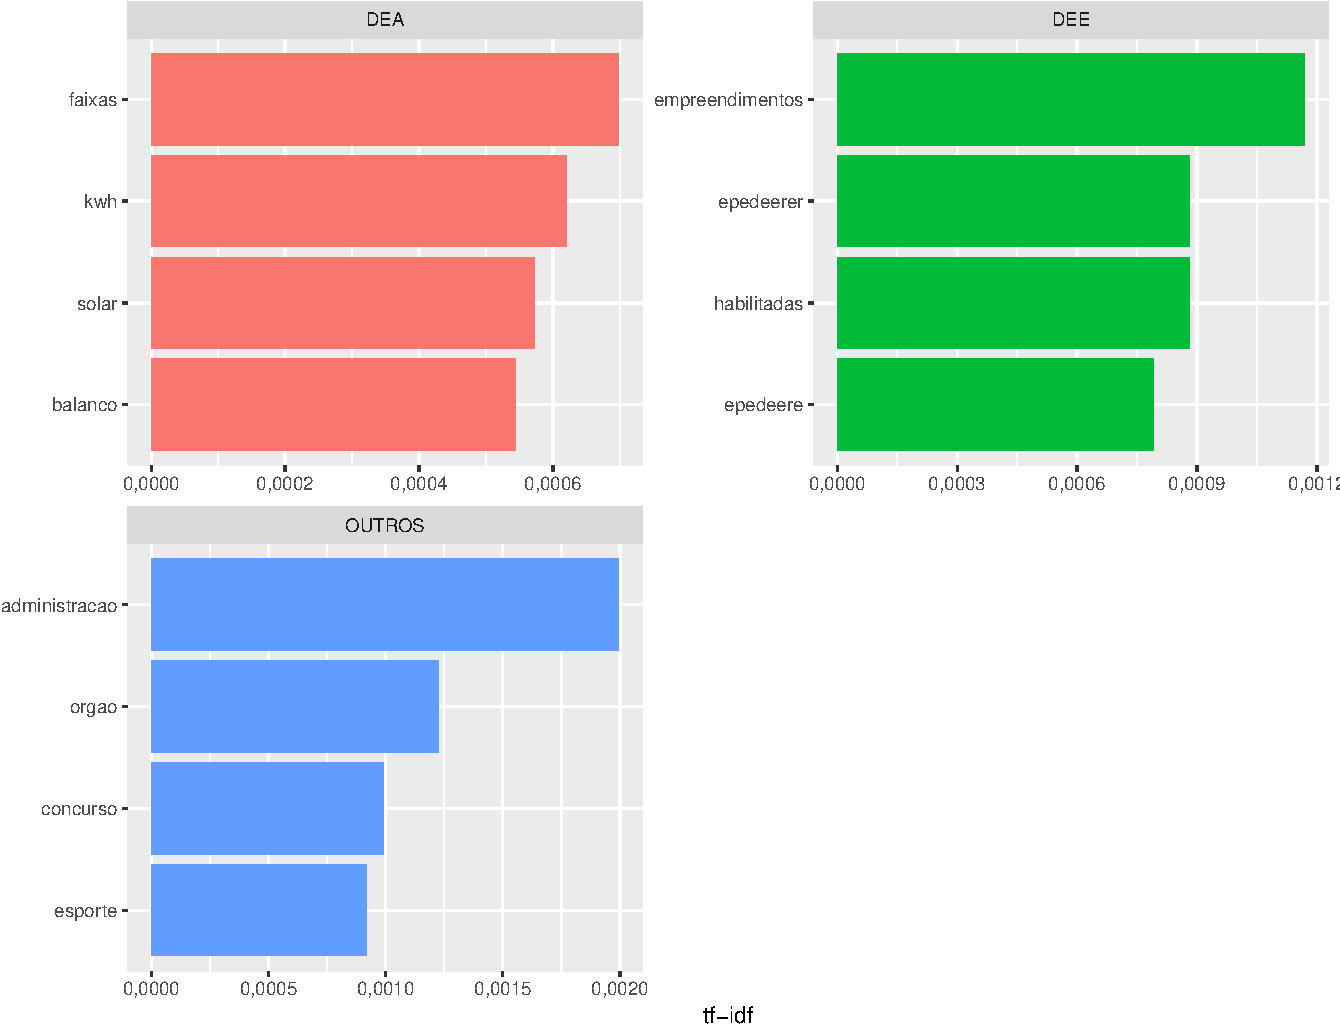
\includegraphics{markdown_v40_test_files/figure-latex/unnamed-chunk-51-1.pdf}

\begin{Shaded}
\begin{Highlighting}[]
\CommentTok{#dev.off()}
\end{Highlighting}
\end{Shaded}

\subsubsection{Stopwords}\label{stopwords}

Com o arquivo de \textbf{stop words} previamente inserido vamos,
primeiramente, transforma-lo em um data\_frame a fim de futuramente
utilizá-lo para extrair do texto palavras em comum.

\paragraph{\texorpdfstring{Freq. de palavras sem \textbf{stopwords} por
diretoria}{Freq. de palavras sem stopwords por diretoria}}\label{freq.-de-palavras-sem-stopwords-por-diretoria}

\begin{Shaded}
\begin{Highlighting}[]
\NormalTok{mystopwords <-}\StringTok{ }\KeywordTok{data_frame}\NormalTok{(}\DataTypeTok{palavra =}\NormalTok{ stopwords_pt)}
\end{Highlighting}
\end{Shaded}

\begin{verbatim}
## Warning: `data_frame()` is deprecated, use `tibble()`.
## This warning is displayed once per session.
\end{verbatim}

\begin{Shaded}
\begin{Highlighting}[]
\NormalTok{diretoria_palavras_noSTOP <-}\StringTok{ }\KeywordTok{anti_join}\NormalTok{(diretoria_palavras_stem3, mystopwords, }
                                       \DataTypeTok{by =} \StringTok{"palavra"}\NormalTok{)}
\end{Highlighting}
\end{Shaded}

\subparagraph{\texorpdfstring{Figura5: Termos mais relevantes por
diretoria pela estatística \textbf{tf\_idf}, após \textbf{stemming} e
sem \textbf{stop
words}}{Figura5: Termos mais relevantes por diretoria pela estatística tf\_idf, após stemming e sem stop words}}\label{figura5-termos-mais-relevantes-por-diretoria-pela-estatistica-tf_idf-apos-stemming-e-sem-stop-words}

Sim, a remoção de \textbf{stop words} não alterou em nada a ordem das 4
palavras mais relevantes de acordo com a estatística.

\begin{Shaded}
\begin{Highlighting}[]
\CommentTok{#diretoria_palavras_noSTOP_noSTOP}
\NormalTok{plot_diretoria_palavras_noSTOP <-}\StringTok{ }\NormalTok{diretoria_palavras_noSTOP }\OperatorTok
\StringTok{  }\KeywordTok{bind_tf_idf}\NormalTok{(palavra, DIRETORIA, n) }\OperatorTok
\StringTok{  }\KeywordTok{arrange}\NormalTok{(}\KeywordTok{desc}\NormalTok{(tf_idf)) }\OperatorTok
\StringTok{  }\KeywordTok{mutate}\NormalTok{(}\DataTypeTok{word =} \KeywordTok{factor}\NormalTok{(palavra, }\DataTypeTok{levels =} \KeywordTok{rev}\NormalTok{(}\KeywordTok{unique}\NormalTok{(palavra)))) }\OperatorTok
\StringTok{  }\KeywordTok{mutate}\NormalTok{(}\DataTypeTok{DIRETORIA =} \KeywordTok{factor}\NormalTok{(DIRETORIA, }\DataTypeTok{levels =} \KeywordTok{c}\NormalTok{(}\StringTok{"DEA"}\NormalTok{,}\StringTok{"DEE"}\NormalTok{,}\StringTok{"OUTROS"}\NormalTok{)))}
\CommentTok{#plot_diretoria_palavras_noSTOP}
\CommentTok{#windows.options(width=10, height=10)}
\CommentTok{#jpeg("03_freq_palavras_dir_nostop.jpeg")}
\NormalTok{plot_diretoria_palavras_noSTOP }\OperatorTok
\StringTok{  }\KeywordTok{group_by}\NormalTok{(DIRETORIA) }\OperatorTok
\StringTok{  }\KeywordTok{top_n}\NormalTok{(}\DecValTok{4}\NormalTok{, tf_idf) }\OperatorTok
\StringTok{  }\KeywordTok{ungroup}\NormalTok{() }\OperatorTok
\StringTok{  }\KeywordTok{mutate}\NormalTok{(}\DataTypeTok{palavra =} \KeywordTok{reorder}\NormalTok{(palavra, tf_idf)) }\OperatorTok
\StringTok{  }\KeywordTok{ggplot}\NormalTok{(}\KeywordTok{aes}\NormalTok{(palavra, tf_idf, }\DataTypeTok{fill =}\NormalTok{ DIRETORIA)) }\OperatorTok{+}
\StringTok{  }\KeywordTok{geom_col}\NormalTok{(}\DataTypeTok{show.legend =} \OtherTok{FALSE}\NormalTok{) }\OperatorTok{+}
\StringTok{  }\KeywordTok{labs}\NormalTok{(}\DataTypeTok{x =} \OtherTok{NULL}\NormalTok{, }\DataTypeTok{y =} \StringTok{"tf-idf"}\NormalTok{) }\OperatorTok{+}
\StringTok{  }\KeywordTok{facet_wrap}\NormalTok{(}\OperatorTok{~}\NormalTok{DIRETORIA, }\DataTypeTok{ncol =} \DecValTok{2}\NormalTok{, }\DataTypeTok{scales =} \StringTok{"free"}\NormalTok{) }\OperatorTok{+}
\StringTok{  }\KeywordTok{coord_flip}\NormalTok{() }\OperatorTok{+}\StringTok{ }
\StringTok{  }\KeywordTok{scale_y_continuous}\NormalTok{(}\DataTypeTok{labels=}\NormalTok{gcomma)}
\end{Highlighting}
\end{Shaded}

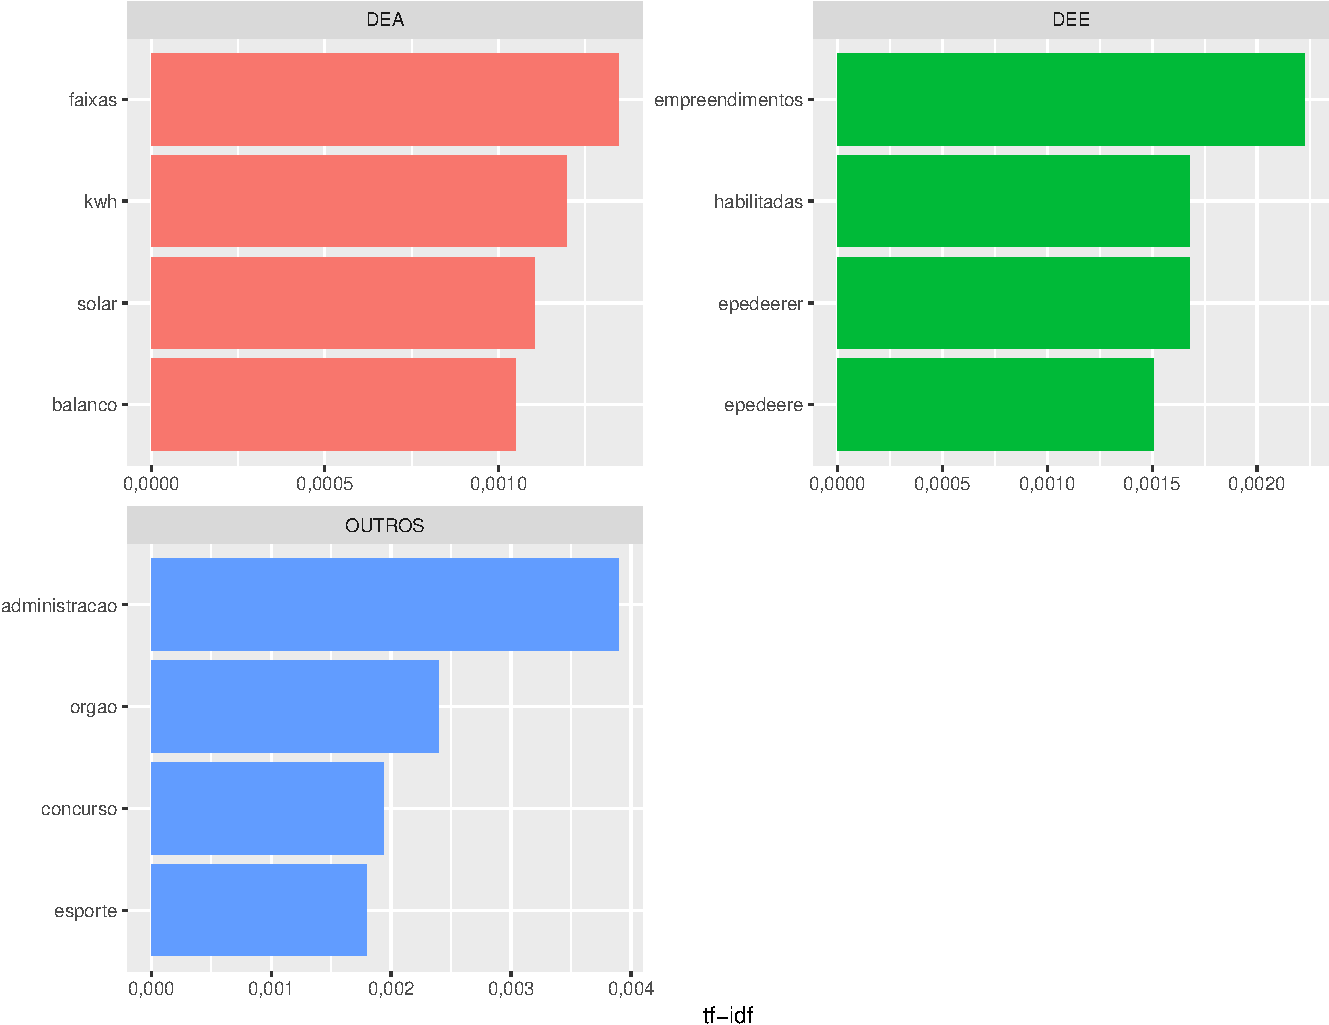
\includegraphics{markdown_v40_test_files/figure-latex/03_freq_palavras_dir_nostop-1.pdf}

\begin{Shaded}
\begin{Highlighting}[]
\CommentTok{#dev.off()}
\end{Highlighting}
\end{Shaded}

\subparagraph{Wordcloud2 - DEE}\label{wordcloud2---dee}

\begin{Shaded}
\begin{Highlighting}[]
\NormalTok{set.seed(6423)}
\NormalTok{plot_diretoria_palavras_noSTOP %>%}
\NormalTok{  filter(DIRETORIA == }\StringTok{"DEE"}\NormalTok{) %>%}
\NormalTok{  select(word = palavra, freq = tf_idf) %>%}
\NormalTok{  mutate(word = as.factor(word)) %>%}
  \CommentTok{#top_n(150, freq) %>%}
\NormalTok{  as.data.frame() %>%}
\NormalTok{  wordcloud2(shuffle = TRUE, color = }\StringTok{"random-dark"}\NormalTok{, shape = }\StringTok{"circle"}\NormalTok{, size = 1.10)}
\end{Highlighting}
\end{Shaded}

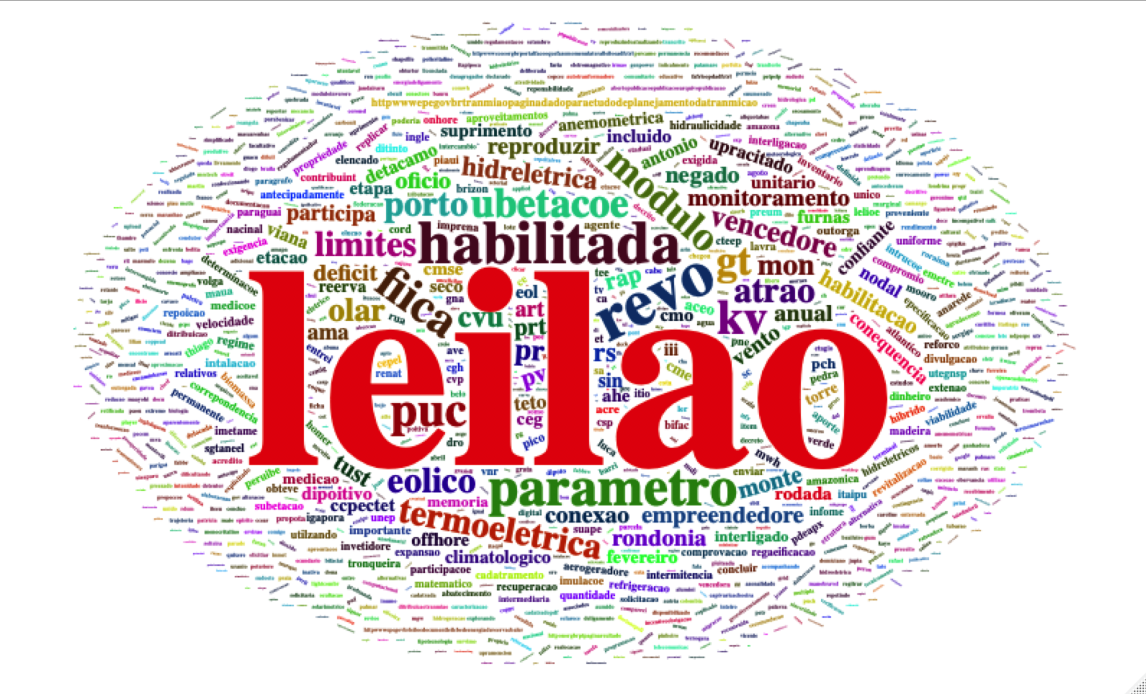
\includegraphics[width=600px]{/Users/ewersonpimenta/Desktop/ESIC_TCC/FINAL/RMARKDOWN/IMAGENS/WORDCLOUDS/01.ONEGRAM_wordcloud2_DEE01}

\subparagraph{Wordcloud2 - DEA}\label{wordcloud2---dea}

\begin{Shaded}
\begin{Highlighting}[]
\NormalTok{set.seed(6423)}
\NormalTok{plot_diretoria_palavras_noSTOP %>%}
\NormalTok{  filter(DIRETORIA == }\StringTok{"DEA"}\NormalTok{) %>%}
\NormalTok{  select(word = palavra, freq = tf_idf) %>%}
\NormalTok{  mutate(word = as.factor(word)) %>%}
  \CommentTok{#top_n(150, freq) %>%}
\NormalTok{  as.data.frame() %>%}
\NormalTok{  wordcloud2(shuffle = TRUE, color = }\StringTok{"random-dark"}\NormalTok{, shape = }\StringTok{"circle"}\NormalTok{, size = .25)}
\end{Highlighting}
\end{Shaded}

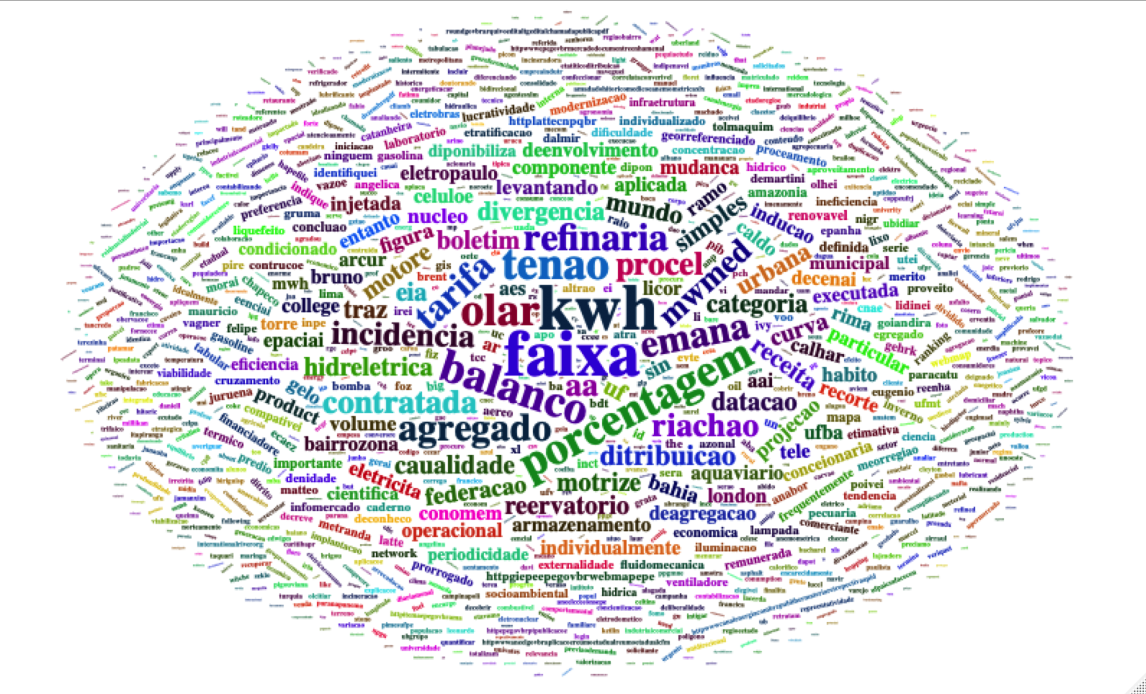
\includegraphics[width=600px]{/Users/ewersonpimenta/Desktop/ESIC_TCC/FINAL/RMARKDOWN/IMAGENS/WORDCLOUDS/01.ONEGRAM_wordcloud2_DEA01}

\subparagraph{Wordcloud2 - OUTROS}\label{wordcloud2---outros}

\begin{Shaded}
\begin{Highlighting}[]
\NormalTok{set.seed(6423)}
\NormalTok{plot_diretoria_palavras_noSTOP %>%}
\NormalTok{  filter(DIRETORIA == }\StringTok{"OUTROS"}\NormalTok{) %>%}
\NormalTok{  select(word = palavra, freq = tf_idf) %>%}
\NormalTok{  mutate(word = as.factor(word)) %>%}
  \CommentTok{#top_n(150, freq) %>%}
\NormalTok{  as.data.frame() %>%}
\NormalTok{  wordcloud2(shuffle = TRUE, color = }\StringTok{"random-dark"}\NormalTok{, shape = }\StringTok{"circle"}\NormalTok{, size = 0.35)}
\end{Highlighting}
\end{Shaded}

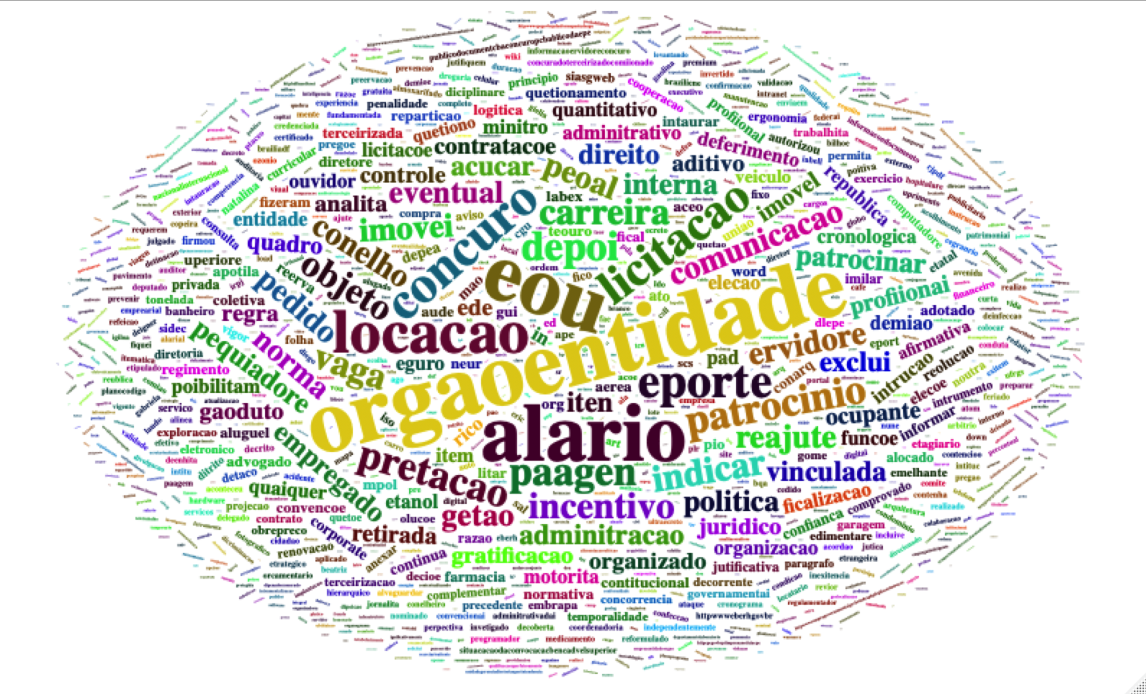
\includegraphics[width=600px]{/Users/ewersonpimenta/Desktop/ESIC_TCC/FINAL/RMARKDOWN/IMAGENS/WORDCLOUDS/01.ONEGRAM_wordcloud2_OUTROS01}

\paragraph{Comparação de frequências dois a dois (sem stopwords e com
stemming)}\label{comparacao-de-frequencias-dois-a-dois-sem-stopwords-e-com-stemming}

Vamos agora comparar a frequência de palavras entre diretorias. Antes
disso, vamos criar documentos de texto no formato tidy separadamente
para cada uma das 3 cateorias: \emph{DEA}, \emph{DEE} e \emph{OUTROS}.

\paragraph{Gráficos de comparação de frequência de palavras por
diretorias (2 a
2)}\label{graficos-de-comparacao-de-frequencia-de-palavras-por-diretorias-2-a-2}

\texttt{COM\ STOPWORDS}

É importante ressaltar que os gráficos a seguir mostram, apenas, a
comparação de frequência de palavras existentes em ambas diretorias. Ou
seja, palavras existentes em apenas uma diretoria serão desconsideradas
para a geração destes.

\begin{Shaded}
\begin{Highlighting}[]
\NormalTok{PROP_PALAVRA =}\StringTok{ }\NormalTok{diretoria_palavras_noSTOP }\OperatorTok
\StringTok{    }\CommentTok{#mutate(palavra = str_extract(palavra, "[a-z']+")) %>%}
\StringTok{    }\KeywordTok{mutate}\NormalTok{(}\DataTypeTok{proportion =}\NormalTok{ n }\OperatorTok{/}\StringTok{ }\KeywordTok{sum}\NormalTok{(n)) }\OperatorTok
\StringTok{    }\KeywordTok{select}\NormalTok{(}\OperatorTok{-}\NormalTok{n) }\OperatorTok
\StringTok{    }\KeywordTok{spread}\NormalTok{(DIRETORIA, proportion)}
\end{Highlighting}
\end{Shaded}

\begin{itemize}
\tightlist
\item
  DEE X DEA
\end{itemize}

\begin{Shaded}
\begin{Highlighting}[]
\NormalTok{freq00 <-}\StringTok{ }\NormalTok{PROP_PALAVRA }\OperatorTok
\StringTok{    }\KeywordTok{gather}\NormalTok{(DIRETORIA, proportion, }\KeywordTok{c}\NormalTok{(}\StringTok{`}\DataTypeTok{DEA}\StringTok{`}\NormalTok{))}
  
  \KeywordTok{library}\NormalTok{(scales)}
  \CommentTok{# expect a warning about rows with missing values being removed}
  \KeywordTok{ggplot}\NormalTok{(freq00, }\KeywordTok{aes}\NormalTok{(}\DataTypeTok{x =}\NormalTok{ proportion, }\DataTypeTok{y =} \StringTok{`}\DataTypeTok{DEE}\StringTok{`}\NormalTok{,}
                        \DataTypeTok{color =} \KeywordTok{abs}\NormalTok{(}\StringTok{`}\DataTypeTok{DEE}\StringTok{`} \OperatorTok{-}\StringTok{ }\NormalTok{proportion))) }\OperatorTok{+}
\StringTok{    }\KeywordTok{geom_abline}\NormalTok{(}\DataTypeTok{color =} \StringTok{"gray40"}\NormalTok{, }\DataTypeTok{lty =} \DecValTok{2}\NormalTok{) }\OperatorTok{+}
\StringTok{    }\KeywordTok{geom_jitter}\NormalTok{(}\DataTypeTok{alpha =} \FloatTok{0.1}\NormalTok{, }\DataTypeTok{size =} \FloatTok{2.5}\NormalTok{, }\DataTypeTok{width =} \FloatTok{0.3}\NormalTok{, }\DataTypeTok{height =} \FloatTok{0.3}\NormalTok{) }\OperatorTok{+}
\StringTok{    }\KeywordTok{geom_text}\NormalTok{(}\KeywordTok{aes}\NormalTok{(}\DataTypeTok{label =}\NormalTok{ palavra), }\DataTypeTok{check_overlap =} \OtherTok{TRUE}\NormalTok{, }\DataTypeTok{vjust =} \FloatTok{1.5}\NormalTok{) }\OperatorTok{+}
\StringTok{    }\KeywordTok{scale_x_log10}\NormalTok{(}\DataTypeTok{labels =} \KeywordTok{percent_format}\NormalTok{(}\DataTypeTok{big.mark =} \StringTok{"."}\NormalTok{, }\DataTypeTok{decimal.mark =} \StringTok{","}\NormalTok{, }
                                          \DataTypeTok{accuracy =} \DecValTok{1}\NormalTok{), }\DataTypeTok{limits =} \KeywordTok{c}\NormalTok{(}\OtherTok{NA}\NormalTok{, }\FloatTok{0.01}\NormalTok{)) }\OperatorTok{+}
\StringTok{    }\KeywordTok{scale_y_log10}\NormalTok{(}\DataTypeTok{labels =} \KeywordTok{percent_format}\NormalTok{(}\DataTypeTok{big.mark =} \StringTok{"."}\NormalTok{, }\DataTypeTok{decimal.mark =} \StringTok{","}\NormalTok{, }
                                          \DataTypeTok{accuracy =} \DecValTok{1}\NormalTok{), }\DataTypeTok{limits =} \KeywordTok{c}\NormalTok{(}\OtherTok{NA}\NormalTok{, }\FloatTok{0.01}\NormalTok{)) }\OperatorTok{+}
\StringTok{    }\KeywordTok{scale_color_gradient}\NormalTok{(}\DataTypeTok{limits =} \KeywordTok{c}\NormalTok{(}\DecValTok{0}\NormalTok{, }\FloatTok{0.001}\NormalTok{),}
                         \DataTypeTok{low =} \StringTok{"darkslategray4"}\NormalTok{, }\DataTypeTok{high =} \StringTok{"gray75"}\NormalTok{) }\OperatorTok{+}
\StringTok{    }\KeywordTok{facet_wrap}\NormalTok{(}\OperatorTok{~}\NormalTok{DIRETORIA, }\DataTypeTok{ncol =} \DecValTok{1}\NormalTok{) }\OperatorTok{+}
\StringTok{    }\KeywordTok{theme}\NormalTok{(}\DataTypeTok{legend.position=}\StringTok{"none"}\NormalTok{) }\OperatorTok{+}
\StringTok{    }\KeywordTok{labs}\NormalTok{(}\DataTypeTok{y =} \StringTok{"DEE"}\NormalTok{, }\DataTypeTok{x =} \OtherTok{NULL}\NormalTok{)}
\end{Highlighting}
\end{Shaded}

\begin{verbatim}
## Warning: Removed 2143 rows containing missing values (geom_point).
\end{verbatim}

\begin{verbatim}
## Warning: Removed 2142 rows containing missing values (geom_text).
\end{verbatim}

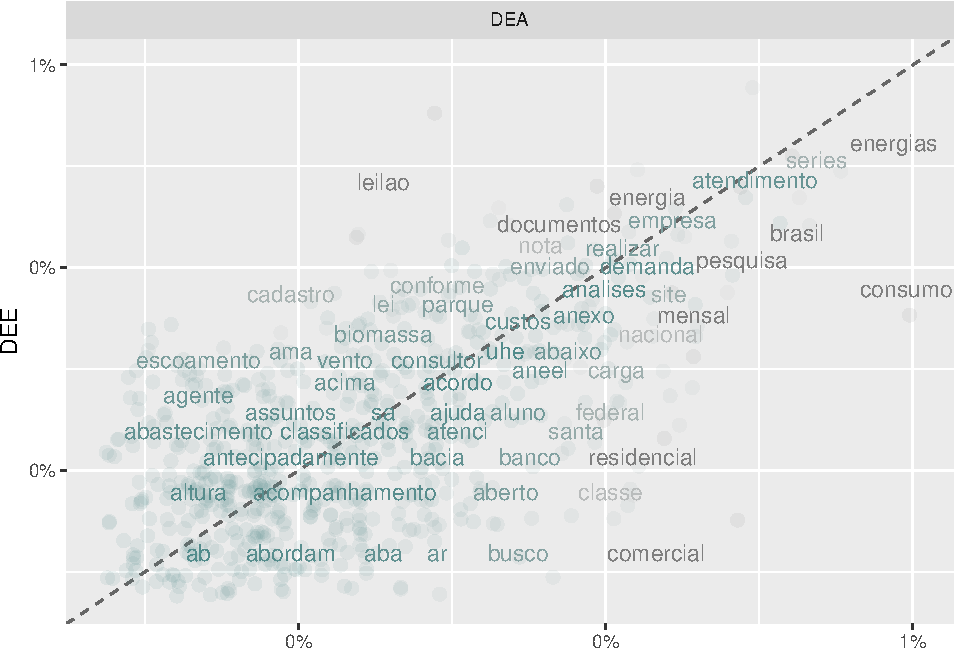
\includegraphics{markdown_v40_test_files/figure-latex/unnamed-chunk-58-1.pdf}

\begin{Shaded}
\begin{Highlighting}[]
\KeywordTok{cor.test}\NormalTok{(}\DataTypeTok{data =}\NormalTok{ freq00[freq00}\OperatorTok{$}\NormalTok{DIRETORIA }\OperatorTok{==}\StringTok{ "DEA"}\NormalTok{,],}
             \OperatorTok{~}\StringTok{ }\NormalTok{proportion }\OperatorTok{+}\StringTok{ `}\DataTypeTok{DEE}\StringTok{`}\NormalTok{)}
\end{Highlighting}
\end{Shaded}

\begin{verbatim}
## 
##  Pearson's product-moment correlation
## 
## data:  proportion and DEE
## t = 138.38, df = 647, p-value < 2.2e-16
## alternative hypothesis: true correlation is not equal to 0
## 95 percent confidence interval:
##  0.9808000 0.9858601
## sample estimates:
##       cor 
## 0.9835216
\end{verbatim}

\begin{itemize}
\tightlist
\item
  DEE X OUTROS
\end{itemize}

\begin{Shaded}
\begin{Highlighting}[]
\NormalTok{freq03 <-}\StringTok{ }\NormalTok{PROP_PALAVRA }\OperatorTok
\StringTok{    }\KeywordTok{gather}\NormalTok{(DIRETORIA, proportion, }\KeywordTok{c}\NormalTok{(}\StringTok{`}\DataTypeTok{OUTROS}\StringTok{`}\NormalTok{))}
  
  \KeywordTok{library}\NormalTok{(scales)}
  \CommentTok{# expect a warning about rows with missing values being removed}
  \KeywordTok{ggplot}\NormalTok{(freq03, }\KeywordTok{aes}\NormalTok{(}\DataTypeTok{x =}\NormalTok{ proportion, }\DataTypeTok{y =} \StringTok{`}\DataTypeTok{DEE}\StringTok{`}\NormalTok{,}
                        \DataTypeTok{color =} \KeywordTok{abs}\NormalTok{(}\StringTok{`}\DataTypeTok{DEE}\StringTok{`} \OperatorTok{-}\StringTok{ }\NormalTok{proportion))) }\OperatorTok{+}
\StringTok{    }\KeywordTok{geom_abline}\NormalTok{(}\DataTypeTok{color =} \StringTok{"gray40"}\NormalTok{, }\DataTypeTok{lty =} \DecValTok{2}\NormalTok{) }\OperatorTok{+}
\StringTok{    }\KeywordTok{geom_jitter}\NormalTok{(}\DataTypeTok{alpha =} \FloatTok{0.1}\NormalTok{, }\DataTypeTok{size =} \FloatTok{2.5}\NormalTok{, }\DataTypeTok{width =} \FloatTok{0.3}\NormalTok{, }\DataTypeTok{height =} \FloatTok{0.3}\NormalTok{) }\OperatorTok{+}
\StringTok{    }\KeywordTok{geom_text}\NormalTok{(}\KeywordTok{aes}\NormalTok{(}\DataTypeTok{label =}\NormalTok{ palavra), }\DataTypeTok{check_overlap =} \OtherTok{TRUE}\NormalTok{, }\DataTypeTok{vjust =} \FloatTok{1.5}\NormalTok{) }\OperatorTok{+}
\StringTok{    }\KeywordTok{scale_x_log10}\NormalTok{(}\DataTypeTok{labels =} \KeywordTok{percent_format}\NormalTok{(}\DataTypeTok{big.mark =} \StringTok{"."}\NormalTok{, }\DataTypeTok{decimal.mark =} \StringTok{","}\NormalTok{, }
                                          \DataTypeTok{accuracy =} \DecValTok{1}\NormalTok{), }\DataTypeTok{limits =} \KeywordTok{c}\NormalTok{(}\OtherTok{NA}\NormalTok{, }\FloatTok{0.01}\NormalTok{)) }\OperatorTok{+}
\StringTok{    }\KeywordTok{scale_y_log10}\NormalTok{(}\DataTypeTok{labels =} \KeywordTok{percent_format}\NormalTok{(}\DataTypeTok{big.mark =} \StringTok{"."}\NormalTok{, }\DataTypeTok{decimal.mark =} \StringTok{","}\NormalTok{, }
                                          \DataTypeTok{accuracy =} \DecValTok{1}\NormalTok{), }\DataTypeTok{limits =} \KeywordTok{c}\NormalTok{(}\OtherTok{NA}\NormalTok{, }\FloatTok{0.01}\NormalTok{)) }\OperatorTok{+}
\StringTok{    }\KeywordTok{scale_color_gradient}\NormalTok{(}\DataTypeTok{limits =} \KeywordTok{c}\NormalTok{(}\DecValTok{0}\NormalTok{, }\FloatTok{0.001}\NormalTok{),}
                         \DataTypeTok{low =} \StringTok{"darkslategray4"}\NormalTok{, }\DataTypeTok{high =} \StringTok{"gray75"}\NormalTok{) }\OperatorTok{+}
\StringTok{    }\KeywordTok{facet_wrap}\NormalTok{(}\OperatorTok{~}\NormalTok{DIRETORIA, }\DataTypeTok{ncol =} \DecValTok{1}\NormalTok{) }\OperatorTok{+}
\StringTok{    }\KeywordTok{theme}\NormalTok{(}\DataTypeTok{legend.position=}\StringTok{"none"}\NormalTok{) }\OperatorTok{+}
\StringTok{    }\KeywordTok{labs}\NormalTok{(}\DataTypeTok{y =} \StringTok{"DEE"}\NormalTok{, }\DataTypeTok{x =} \OtherTok{NULL}\NormalTok{)}
\end{Highlighting}
\end{Shaded}

\begin{verbatim}
## Warning: Removed 2217 rows containing missing values (geom_point).
\end{verbatim}

\begin{verbatim}
## Warning: Removed 2217 rows containing missing values (geom_text).
\end{verbatim}

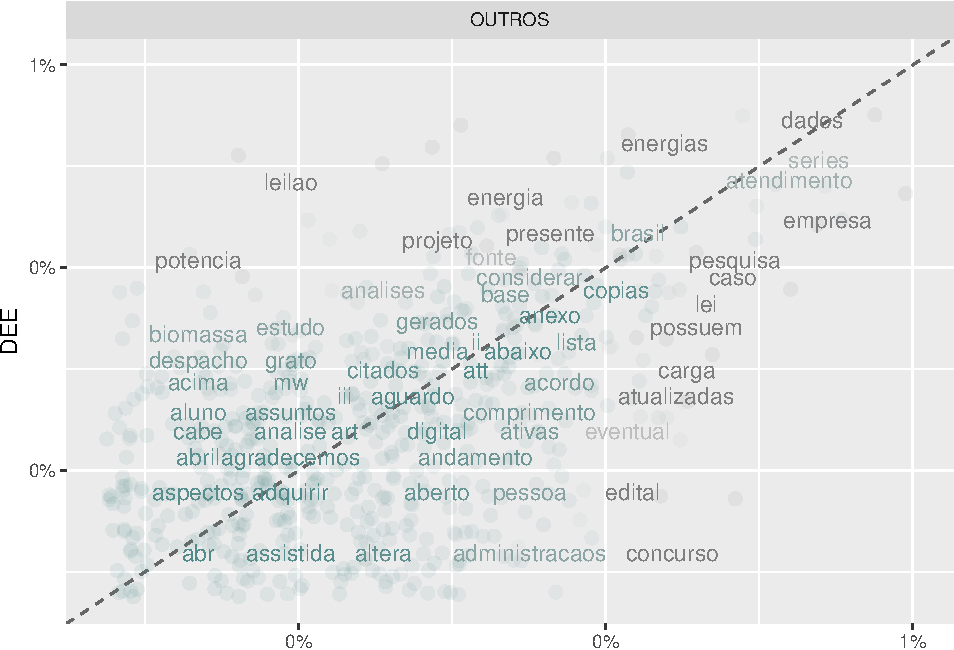
\includegraphics{markdown_v40_test_files/figure-latex/unnamed-chunk-60-1.pdf}

\begin{Shaded}
\begin{Highlighting}[]
\KeywordTok{cor.test}\NormalTok{(}\DataTypeTok{data =}\NormalTok{ freq03[freq03}\OperatorTok{$}\NormalTok{DIRETORIA }\OperatorTok{==}\StringTok{ "OUTROS"}\NormalTok{,],}
             \OperatorTok{~}\StringTok{ }\NormalTok{proportion }\OperatorTok{+}\StringTok{ `}\DataTypeTok{DEE}\StringTok{`}\NormalTok{)}
\end{Highlighting}
\end{Shaded}

\begin{verbatim}
## 
##  Pearson's product-moment correlation
## 
## data:  proportion and DEE
## t = 147.24, df = 571, p-value < 2.2e-16
## alternative hypothesis: true correlation is not equal to 0
## 95 percent confidence interval:
##  0.9847981 0.9890299
## sample estimates:
##      cor 
## 0.987085
\end{verbatim}

\begin{Shaded}
\begin{Highlighting}[]
\FunctionTok{Warning messages:}
\FunctionTok{1:}\AttributeTok{ Removed 4273 rows containing missing values (geom_point). }
\FunctionTok{2:}\AttributeTok{ Removed 4274 rows containing missing values (geom_text).}
\end{Highlighting}
\end{Shaded}

\begin{itemize}
\tightlist
\item
  DEA X OUTROS
\end{itemize}

\begin{Shaded}
\begin{Highlighting}[]
\NormalTok{freq06 <-}\StringTok{ }\NormalTok{PROP_PALAVRA }\OperatorTok
\StringTok{    }\KeywordTok{gather}\NormalTok{(DIRETORIA, proportion, }\KeywordTok{c}\NormalTok{(}\StringTok{`}\DataTypeTok{OUTROS}\StringTok{`}\NormalTok{))}
  
  \KeywordTok{library}\NormalTok{(scales)}
  \CommentTok{# expect a warning about rows with missing values being removed}
  \KeywordTok{ggplot}\NormalTok{(freq06, }\KeywordTok{aes}\NormalTok{(}\DataTypeTok{x =}\NormalTok{ proportion, }\DataTypeTok{y =} \StringTok{`}\DataTypeTok{DEA}\StringTok{`}\NormalTok{,}
                        \DataTypeTok{color =} \KeywordTok{abs}\NormalTok{(}\StringTok{`}\DataTypeTok{DEA}\StringTok{`} \OperatorTok{-}\StringTok{ }\NormalTok{proportion))) }\OperatorTok{+}
\StringTok{    }\KeywordTok{geom_abline}\NormalTok{(}\DataTypeTok{color =} \StringTok{"gray40"}\NormalTok{, }\DataTypeTok{lty =} \DecValTok{2}\NormalTok{) }\OperatorTok{+}
\StringTok{    }\KeywordTok{geom_jitter}\NormalTok{(}\DataTypeTok{alpha =} \FloatTok{0.1}\NormalTok{, }\DataTypeTok{size =} \FloatTok{2.5}\NormalTok{, }\DataTypeTok{width =} \FloatTok{0.3}\NormalTok{, }\DataTypeTok{height =} \FloatTok{0.3}\NormalTok{) }\OperatorTok{+}
\StringTok{    }\KeywordTok{geom_text}\NormalTok{(}\KeywordTok{aes}\NormalTok{(}\DataTypeTok{label =}\NormalTok{ palavra), }\DataTypeTok{check_overlap =} \OtherTok{TRUE}\NormalTok{, }\DataTypeTok{vjust =} \FloatTok{1.5}\NormalTok{) }\OperatorTok{+}
\StringTok{    }\KeywordTok{scale_x_log10}\NormalTok{(}\DataTypeTok{labels =} \KeywordTok{percent_format}\NormalTok{(}\DataTypeTok{big.mark =} \StringTok{"."}\NormalTok{, }\DataTypeTok{decimal.mark =} \StringTok{","}\NormalTok{, }
                                          \DataTypeTok{accuracy =} \DecValTok{1}\NormalTok{), }\DataTypeTok{limits =} \KeywordTok{c}\NormalTok{(}\OtherTok{NA}\NormalTok{, }\FloatTok{0.01}\NormalTok{)) }\OperatorTok{+}
\StringTok{    }\KeywordTok{scale_y_log10}\NormalTok{(}\DataTypeTok{labels =} \KeywordTok{percent_format}\NormalTok{(}\DataTypeTok{big.mark =} \StringTok{"."}\NormalTok{, }\DataTypeTok{decimal.mark =} \StringTok{","}\NormalTok{, }
                                          \DataTypeTok{accuracy =} \DecValTok{1}\NormalTok{), }\DataTypeTok{limits =} \KeywordTok{c}\NormalTok{(}\OtherTok{NA}\NormalTok{, }\FloatTok{0.01}\NormalTok{)) }\OperatorTok{+}
\StringTok{    }\KeywordTok{scale_color_gradient}\NormalTok{(}\DataTypeTok{limits =} \KeywordTok{c}\NormalTok{(}\DecValTok{0}\NormalTok{, }\FloatTok{0.001}\NormalTok{),}
                         \DataTypeTok{low =} \StringTok{"darkslategray4"}\NormalTok{, }\DataTypeTok{high =} \StringTok{"gray75"}\NormalTok{) }\OperatorTok{+}
\StringTok{    }\KeywordTok{facet_wrap}\NormalTok{(}\OperatorTok{~}\NormalTok{DIRETORIA, }\DataTypeTok{ncol =} \DecValTok{1}\NormalTok{) }\OperatorTok{+}
\StringTok{    }\KeywordTok{theme}\NormalTok{(}\DataTypeTok{legend.position=}\StringTok{"none"}\NormalTok{) }\OperatorTok{+}
\StringTok{    }\KeywordTok{labs}\NormalTok{(}\DataTypeTok{y =} \StringTok{"DEA"}\NormalTok{, }\DataTypeTok{x =} \OtherTok{NULL}\NormalTok{)}
\end{Highlighting}
\end{Shaded}

\begin{verbatim}
## Warning: Removed 2213 rows containing missing values (geom_point).
\end{verbatim}

\begin{verbatim}
## Warning: Removed 2212 rows containing missing values (geom_text).
\end{verbatim}

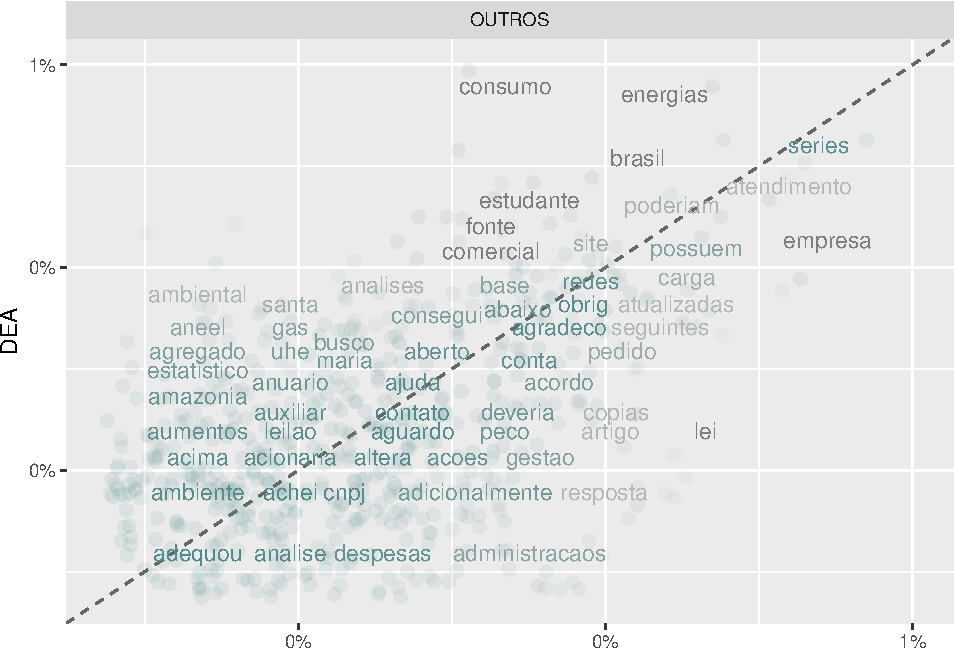
\includegraphics{markdown_v40_test_files/figure-latex/unnamed-chunk-62-1.pdf}

\begin{Shaded}
\begin{Highlighting}[]
\FunctionTok{Warning messages:}
\FunctionTok{1:}\AttributeTok{ Removed 4303 rows containing missing values (geom_point). }
\FunctionTok{2:}\AttributeTok{ Removed 4304 rows containing missing values (geom_text). }
\end{Highlighting}
\end{Shaded}

\begin{Shaded}
\begin{Highlighting}[]
\KeywordTok{cor.test}\NormalTok{(}\DataTypeTok{data =}\NormalTok{ freq06[freq06}\OperatorTok{$}\NormalTok{DIRETORIA }\OperatorTok{==}\StringTok{ "OUTROS"}\NormalTok{,],}
             \OperatorTok{~}\StringTok{ }\NormalTok{proportion }\OperatorTok{+}\StringTok{ `}\DataTypeTok{DEA}\StringTok{`}\NormalTok{)}
\end{Highlighting}
\end{Shaded}

\begin{verbatim}
## 
##  Pearson's product-moment correlation
## 
## data:  proportion and DEA
## t = 104.61, df = 577, p-value < 2.2e-16
## alternative hypothesis: true correlation is not equal to 0
## 95 percent confidence interval:
##  0.9702007 0.9784153
## sample estimates:
##       cor 
## 0.9746342
\end{verbatim}

\subsubsection{Usando bigram para n=2 palavras por
token}\label{usando-bigram-para-n2-palavras-por-token}

\paragraph{top 6 de palavras por
diretoria}\label{top-6-de-palavras-por-diretoria}

\subparagraph{\texorpdfstring{Figura6: Termos (\textbf{bigram}) mais
relevantes por diretoria pela estatística \textbf{tf\_idf}, após
\textbf{stemming} e sem \textbf{stop
words}}{Figura6: Termos (bigram) mais relevantes por diretoria pela estatística tf\_idf, após stemming e sem stop words}}\label{figura6-termos-bigram-mais-relevantes-por-diretoria-pela-estatistica-tf_idf-apos-stemming-e-sem-stop-words}

\begin{Shaded}
\begin{Highlighting}[]
\NormalTok{diretoria_palavras_bigram <-}\StringTok{ }\NormalTok{DB }\OperatorTok
\StringTok{  }\KeywordTok{select}\NormalTok{(DESCRI_PEDIDO1,DIRETORIA) }\OperatorTok
\StringTok{  }\KeywordTok{unnest_tokens}\NormalTok{(BIGRAM, DESCRI_PEDIDO1, }\DataTypeTok{token =} \StringTok{"ngrams"}\NormalTok{, }\DataTypeTok{n =} \DecValTok{2}\NormalTok{) }\OperatorTok
\StringTok{  }\KeywordTok{count}\NormalTok{(DIRETORIA, BIGRAM, }\DataTypeTok{sort =} \OtherTok{TRUE}\NormalTok{) }\OperatorTok
\StringTok{  }\KeywordTok{ungroup}\NormalTok{()}
\CommentTok{#diretoria_palavras_bigram}

\NormalTok{plot_diretoria_palavras_bigram <-}\StringTok{ }\NormalTok{diretoria_palavras_bigram }\OperatorTok
\StringTok{  }\KeywordTok{bind_tf_idf}\NormalTok{(BIGRAM, DIRETORIA, n) }\OperatorTok
\StringTok{  }\KeywordTok{arrange}\NormalTok{(}\KeywordTok{desc}\NormalTok{(tf_idf)) }\OperatorTok
\StringTok{  }\KeywordTok{mutate}\NormalTok{(}\DataTypeTok{BIGRAM =} \KeywordTok{factor}\NormalTok{(BIGRAM, }\DataTypeTok{levels =} \KeywordTok{rev}\NormalTok{(}\KeywordTok{unique}\NormalTok{(BIGRAM)))) }\OperatorTok
\StringTok{  }\KeywordTok{mutate}\NormalTok{(}\DataTypeTok{DIRETORIA =} \KeywordTok{factor}\NormalTok{(DIRETORIA, }\DataTypeTok{levels =} \KeywordTok{c}\NormalTok{(}\StringTok{"DEA"}\NormalTok{,}\StringTok{"DEE"}\NormalTok{,}\StringTok{"OUTROS"}\NormalTok{)))}
\CommentTok{#View(head(plot_diretoria_palavras_bigram))}

\CommentTok{#jpeg("02_freq_palavras_dir.jpeg")}
\NormalTok{plot_diretoria_palavras_bigram }\OperatorTok
\StringTok{  }\KeywordTok{group_by}\NormalTok{(DIRETORIA) }\OperatorTok
\StringTok{  }\KeywordTok{top_n}\NormalTok{(}\DecValTok{6}\NormalTok{, tf_idf) }\OperatorTok
\StringTok{  }\KeywordTok{ungroup}\NormalTok{() }\OperatorTok
\StringTok{  }\KeywordTok{mutate}\NormalTok{(}\DataTypeTok{BIGRAM =} \KeywordTok{reorder}\NormalTok{(BIGRAM, tf_idf)) }\OperatorTok
\StringTok{  }\KeywordTok{ggplot}\NormalTok{(}\KeywordTok{aes}\NormalTok{(BIGRAM, tf_idf, }\DataTypeTok{fill =}\NormalTok{ DIRETORIA)) }\OperatorTok{+}
\StringTok{  }\KeywordTok{geom_col}\NormalTok{(}\DataTypeTok{show.legend =} \OtherTok{FALSE}\NormalTok{) }\OperatorTok{+}
\StringTok{  }\KeywordTok{labs}\NormalTok{(}\DataTypeTok{x =} \OtherTok{NULL}\NormalTok{, }\DataTypeTok{y =} \StringTok{"tf-idf"}\NormalTok{) }\OperatorTok{+}
\StringTok{  }\KeywordTok{facet_wrap}\NormalTok{(}\OperatorTok{~}\NormalTok{DIRETORIA, }\DataTypeTok{ncol =} \DecValTok{2}\NormalTok{, }\DataTypeTok{scales =} \StringTok{"free"}\NormalTok{) }\OperatorTok{+}
\StringTok{  }\KeywordTok{coord_flip}\NormalTok{() }\OperatorTok{+}\StringTok{ }
\StringTok{  }\KeywordTok{scale_y_continuous}\NormalTok{(}\DataTypeTok{labels=}\NormalTok{gcomma)}
\end{Highlighting}
\end{Shaded}

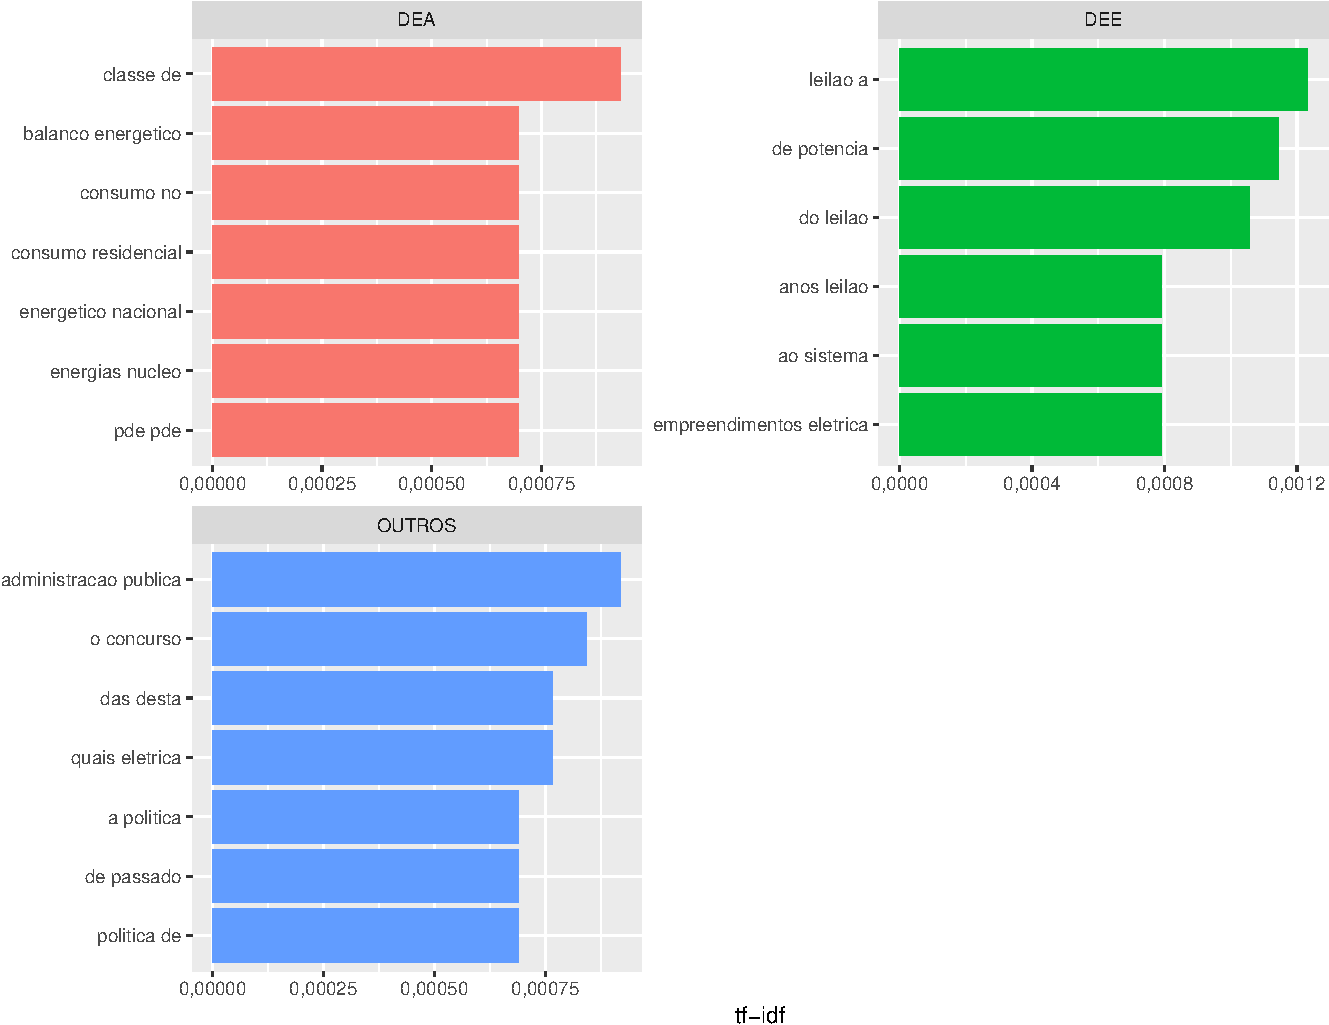
\includegraphics{markdown_v40_test_files/figure-latex/03_freq_palavras_dir-1.pdf}

\begin{Shaded}
\begin{Highlighting}[]
\CommentTok{#dev.off()}
\end{Highlighting}
\end{Shaded}

\subsubsection{Usando bigram para n=3 palavras por
token}\label{usando-bigram-para-n3-palavras-por-token}

\paragraph{Frequência de palavras por
diretoria}\label{frequencia-de-palavras-por-diretoria-1}

\subparagraph{\texorpdfstring{Figura7: Termos (\textbf{trigram}) mais
relevantes por diretoria pela estatística \textbf{tf\_idf}, após
\textbf{stemming} e sem \textbf{stop
words}}{Figura7: Termos (trigram) mais relevantes por diretoria pela estatística tf\_idf, após stemming e sem stop words}}\label{figura7-termos-trigram-mais-relevantes-por-diretoria-pela-estatistica-tf_idf-apos-stemming-e-sem-stop-words}

\begin{Shaded}
\begin{Highlighting}[]
\NormalTok{diretoria_palavras_trigram <-}\StringTok{ }\NormalTok{DB }\OperatorTok
\StringTok{  }\KeywordTok{select}\NormalTok{(DESCRI_PEDIDO1,DIRETORIA) }\OperatorTok
\StringTok{  }\KeywordTok{unnest_tokens}\NormalTok{(TRIGRAM, DESCRI_PEDIDO1, }\DataTypeTok{token =} \StringTok{"ngrams"}\NormalTok{, }\DataTypeTok{n =} \DecValTok{3}\NormalTok{) }\OperatorTok
\StringTok{  }\KeywordTok{count}\NormalTok{(DIRETORIA, TRIGRAM, }\DataTypeTok{sort =} \OtherTok{TRUE}\NormalTok{) }\OperatorTok
\StringTok{  }\KeywordTok{ungroup}\NormalTok{()}
\CommentTok{#diretoria_palavras_trigram}

\NormalTok{plot_diretoria_palavras_trigram <-}\StringTok{ }\NormalTok{diretoria_palavras_trigram }\OperatorTok
\StringTok{  }\KeywordTok{bind_tf_idf}\NormalTok{(TRIGRAM, DIRETORIA, n) }\OperatorTok
\StringTok{  }\KeywordTok{arrange}\NormalTok{(}\KeywordTok{desc}\NormalTok{(tf_idf)) }\OperatorTok
\StringTok{  }\KeywordTok{mutate}\NormalTok{(}\DataTypeTok{TRIGRAM =} \KeywordTok{factor}\NormalTok{(TRIGRAM, }\DataTypeTok{levels =} \KeywordTok{rev}\NormalTok{(}\KeywordTok{unique}\NormalTok{(TRIGRAM)))) }\OperatorTok
\StringTok{  }\KeywordTok{mutate}\NormalTok{(}\DataTypeTok{DIRETORIA =} \KeywordTok{factor}\NormalTok{(DIRETORIA, }\DataTypeTok{levels =} \KeywordTok{c}\NormalTok{(}\StringTok{"DEA"}\NormalTok{,}\StringTok{"DEE"}\NormalTok{,}\StringTok{"OUTROS"}\NormalTok{)))}
\CommentTok{#View(head(plot_diretoria_palavras_trigram))}
\CommentTok{#jpeg("02_freq_palavras_dir.jpeg")}
\NormalTok{plot_diretoria_palavras_trigram }\OperatorTok
\StringTok{  }\KeywordTok{group_by}\NormalTok{(DIRETORIA) }\OperatorTok
\StringTok{  }\KeywordTok{top_n}\NormalTok{(}\DecValTok{5}\NormalTok{, tf_idf) }\OperatorTok
\StringTok{  }\KeywordTok{ungroup}\NormalTok{() }\OperatorTok
\StringTok{  }\KeywordTok{mutate}\NormalTok{(}\DataTypeTok{TRIGRAM =} \KeywordTok{reorder}\NormalTok{(TRIGRAM, tf_idf)) }\OperatorTok
\StringTok{  }\KeywordTok{ggplot}\NormalTok{(}\KeywordTok{aes}\NormalTok{(TRIGRAM, tf_idf, }\DataTypeTok{fill =}\NormalTok{ DIRETORIA)) }\OperatorTok{+}
\StringTok{  }\KeywordTok{geom_col}\NormalTok{(}\DataTypeTok{show.legend =} \OtherTok{FALSE}\NormalTok{) }\OperatorTok{+}
\StringTok{  }\KeywordTok{labs}\NormalTok{(}\DataTypeTok{x =} \OtherTok{NULL}\NormalTok{, }\DataTypeTok{y =} \StringTok{"tf-idf"}\NormalTok{) }\OperatorTok{+}
\StringTok{  }\KeywordTok{facet_wrap}\NormalTok{(}\OperatorTok{~}\NormalTok{DIRETORIA, }\DataTypeTok{ncol =} \DecValTok{2}\NormalTok{, }\DataTypeTok{scales =} \StringTok{"free"}\NormalTok{) }\OperatorTok{+}
\StringTok{  }\KeywordTok{coord_flip}\NormalTok{() }\OperatorTok{+}\StringTok{ }
\StringTok{  }\KeywordTok{scale_y_continuous}\NormalTok{(}\DataTypeTok{labels=}\NormalTok{gcomma)}
\end{Highlighting}
\end{Shaded}

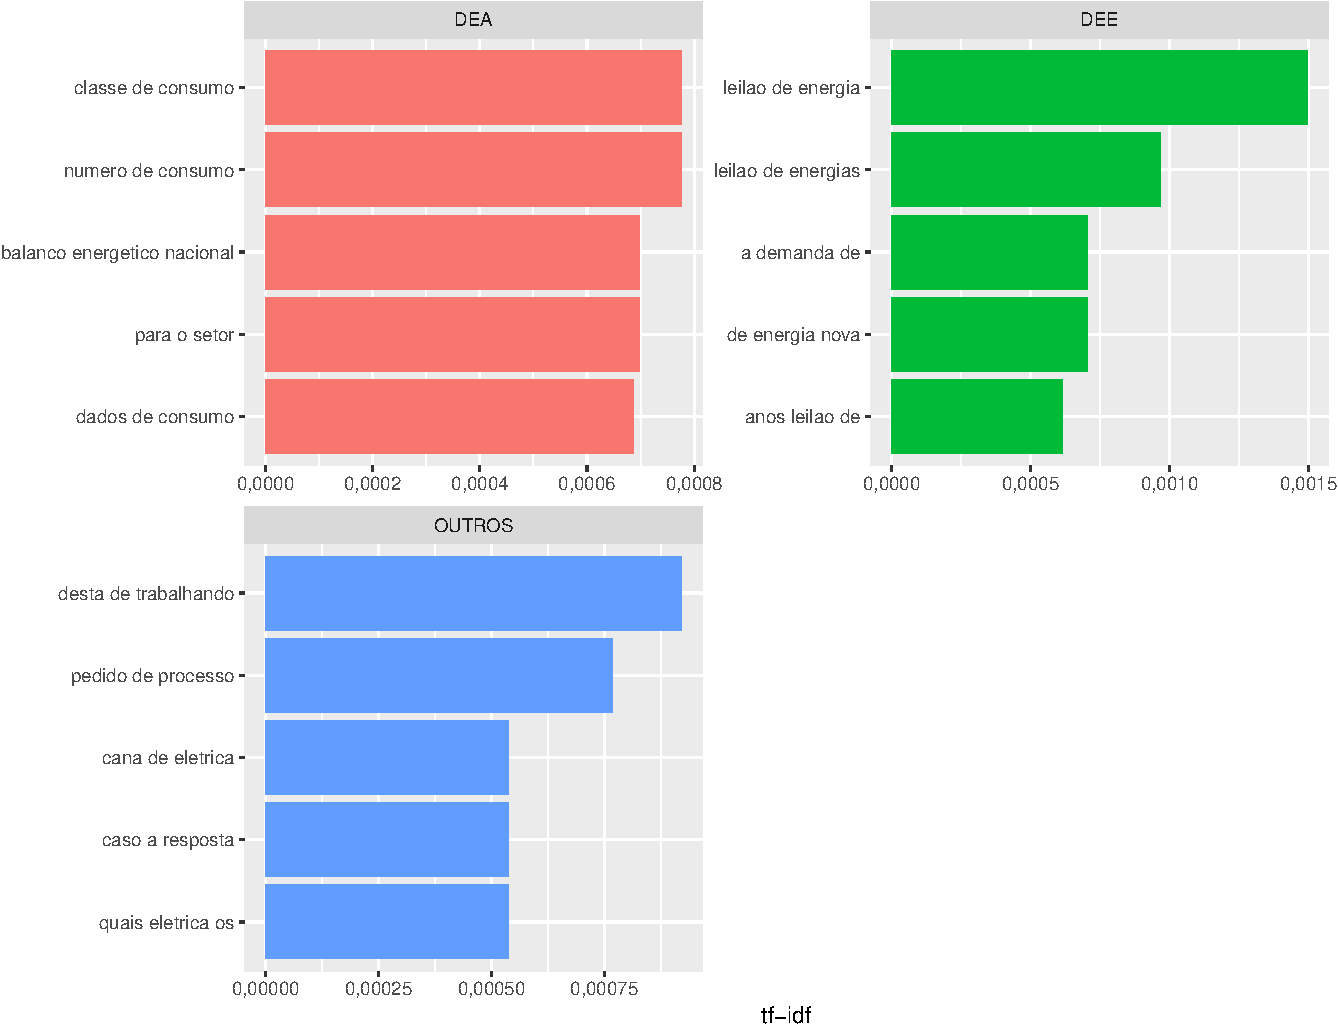
\includegraphics{markdown_v40_test_files/figure-latex/04_freq_palavras_dir-1.pdf}

\begin{Shaded}
\begin{Highlighting}[]
\CommentTok{#dev.off()}
\end{Highlighting}
\end{Shaded}

\subsection{tidy object into document-term
matrix}\label{tidy-object-into-document-term-matrix}

\begin{Shaded}
\begin{Highlighting}[]
\NormalTok{plot_diretoria_palavras <-}\StringTok{ }\NormalTok{diretoria_palavras }\OperatorTok
\StringTok{  }\KeywordTok{bind_tf_idf}\NormalTok{(palavra, DIRETORIA, n) }\OperatorTok
\StringTok{  }\KeywordTok{arrange}\NormalTok{(}\KeywordTok{desc}\NormalTok{(tf_idf)) }\OperatorTok
\StringTok{  }\KeywordTok{mutate}\NormalTok{(}\DataTypeTok{palavra =} \KeywordTok{factor}\NormalTok{(palavra, }\DataTypeTok{levels =} \KeywordTok{rev}\NormalTok{(}\KeywordTok{unique}\NormalTok{(palavra)))) }\OperatorTok
\StringTok{  }\KeywordTok{mutate}\NormalTok{(}\DataTypeTok{DIRETORIA =} \KeywordTok{factor}\NormalTok{(DIRETORIA, }\DataTypeTok{levels =} \KeywordTok{c}\NormalTok{(}\StringTok{"DEA"}\NormalTok{,}\StringTok{"DEE"}\NormalTok{,}\StringTok{"OUTROS"}\NormalTok{)))}

\NormalTok{dtm =}\StringTok{ }\NormalTok{plot_diretoria_palavras }\OperatorTok
\StringTok{  }\KeywordTok{cast_dtm}\NormalTok{(}\DataTypeTok{document =}\NormalTok{ DIRETORIA, }\DataTypeTok{term =}\NormalTok{ palavra, n)}
\end{Highlighting}
\end{Shaded}

\subsubsection{Nuvem de palavras}\label{nuvem-de-palavras}

\paragraph{Nuvem de palavras por diretoria - s/ steeming e/ c/ stopwords
-
onegram}\label{nuvem-de-palavras-por-diretoria---s-steeming-e-c-stopwords---onegram}

\begin{Shaded}
\begin{Highlighting}[]
\CommentTok{#View(head(plot_diretoria_palavras))}
\KeywordTok{library}\NormalTok{(wordcloud)}
\NormalTok{plot_diretorias_tf_dif =}\StringTok{ }\NormalTok{plot_diretoria_palavras }\OperatorTok
\StringTok{  }\KeywordTok{select}\NormalTok{(palavra, tf_idf, DIRETORIA) }\OperatorTok
\StringTok{  }\KeywordTok{mutate}\NormalTok{(}\DataTypeTok{palavra =} \KeywordTok{reorder}\NormalTok{(palavra, tf_idf))}

\NormalTok{## DEE}
\CommentTok{#jpeg("XX_wordclou_tfidf_dir01_DEE.jpeg")}
\NormalTok{nuvem1 =}\StringTok{ }
\StringTok{  }\NormalTok{plot_diretorias_tf_dif }\OperatorTok
\StringTok{  }\KeywordTok{filter}\NormalTok{(DIRETORIA }\OperatorTok{==}\StringTok{ "DEE"}\NormalTok{) }\OperatorTok
\StringTok{  }\KeywordTok{select}\NormalTok{(}\OperatorTok{-}\NormalTok{DIRETORIA, }\DataTypeTok{word =}\NormalTok{ palavra,}\DataTypeTok{freq =}\NormalTok{ tf_idf) }\OperatorTok
\StringTok{  }\CommentTok{#top_n(150, freq) %>%}
\StringTok{  }\KeywordTok{as.data.frame}\NormalTok{() }

\KeywordTok{set.seed}\NormalTok{(}\DecValTok{231321}\NormalTok{)}
\KeywordTok{wordcloud}\NormalTok{(}\DataTypeTok{words =}\NormalTok{ nuvem1}\OperatorTok{$}\NormalTok{word, }\DataTypeTok{freq =}\NormalTok{ nuvem1}\OperatorTok{$}\NormalTok{freq, }\DataTypeTok{min.freq =} \FloatTok{0.2}\NormalTok{,}
          \DataTypeTok{max.words=}\DecValTok{250}\NormalTok{, }\DataTypeTok{random.order=}\OtherTok{FALSE}\NormalTok{, }\DataTypeTok{rot.per=}\FloatTok{0.35}\NormalTok{, }
          \DataTypeTok{colors=}\KeywordTok{brewer.pal}\NormalTok{(}\DecValTok{10}\NormalTok{, }\StringTok{"Dark2"}\NormalTok{))}
\end{Highlighting}
\end{Shaded}

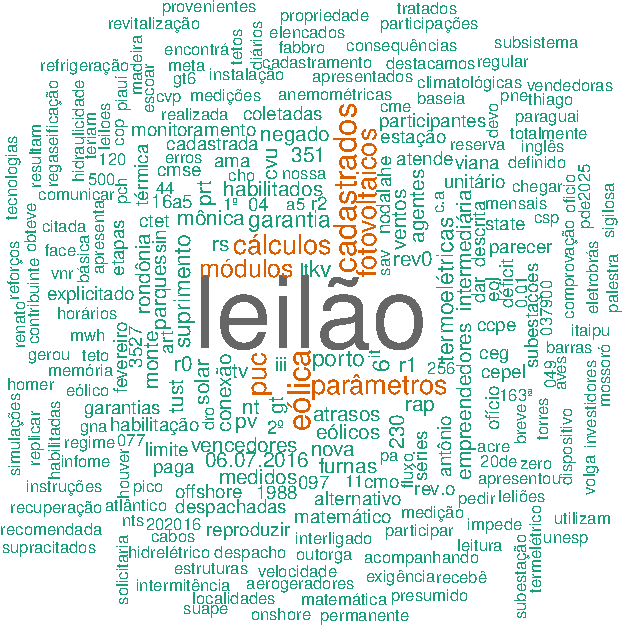
\includegraphics{markdown_v40_test_files/figure-latex/unnamed-chunk-66-1.pdf}

\begin{Shaded}
\begin{Highlighting}[]
\NormalTok{## DEA}
\CommentTok{#jpeg("XX_wordclou_tfidf_dir03_DEA.jpeg")}
\NormalTok{nuvem3 =}\StringTok{ }
\StringTok{  }\NormalTok{plot_diretorias_tf_dif }\OperatorTok
\StringTok{  }\KeywordTok{filter}\NormalTok{(DIRETORIA }\OperatorTok{==}\StringTok{ "DEA"}\NormalTok{) }\OperatorTok
\StringTok{  }\KeywordTok{select}\NormalTok{(}\OperatorTok{-}\NormalTok{DIRETORIA, }\DataTypeTok{word =}\NormalTok{ palavra,}\DataTypeTok{freq =}\NormalTok{ tf_idf) }\OperatorTok
\StringTok{  }\CommentTok{#top_n(150, freq) %>%}
\StringTok{  }\KeywordTok{as.data.frame}\NormalTok{() }

\KeywordTok{set.seed}\NormalTok{(}\DecValTok{231321}\NormalTok{)}
\KeywordTok{wordcloud}\NormalTok{(}\DataTypeTok{words =}\NormalTok{ nuvem3}\OperatorTok{$}\NormalTok{word, }\DataTypeTok{freq =}\NormalTok{ nuvem3}\OperatorTok{$}\NormalTok{freq, }\DataTypeTok{min.freq =} \FloatTok{0.2}\NormalTok{,}
          \DataTypeTok{max.words=}\DecValTok{250}\NormalTok{, }\DataTypeTok{random.order=}\OtherTok{FALSE}\NormalTok{, }\DataTypeTok{rot.per=}\FloatTok{0.35}\NormalTok{, }
          \DataTypeTok{colors=}\KeywordTok{brewer.pal}\NormalTok{(}\DecValTok{10}\NormalTok{, }\StringTok{"Dark2"}\NormalTok{))}
\end{Highlighting}
\end{Shaded}

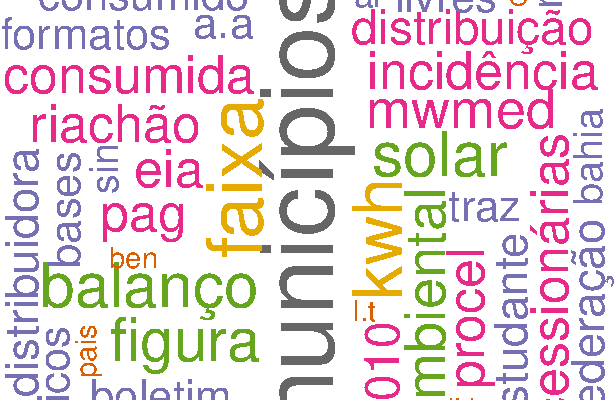
\includegraphics{markdown_v40_test_files/figure-latex/unnamed-chunk-66-2.pdf}

\begin{Shaded}
\begin{Highlighting}[]
\NormalTok{## OUTROS}
\CommentTok{#jpeg("XX_wordclou_tfidf_dir05_OUTROS.jpeg")}
\NormalTok{nuvem5 =}\StringTok{ }
\StringTok{  }\NormalTok{plot_diretorias_tf_dif }\OperatorTok
\StringTok{  }\KeywordTok{filter}\NormalTok{(DIRETORIA }\OperatorTok{==}\StringTok{ "OUTROS"}\NormalTok{) }\OperatorTok
\StringTok{  }\KeywordTok{select}\NormalTok{(}\OperatorTok{-}\NormalTok{DIRETORIA, }\DataTypeTok{word =}\NormalTok{ palavra,}\DataTypeTok{freq =}\NormalTok{ tf_idf) }\OperatorTok
\StringTok{  }\CommentTok{#top_n(150, freq) %>%}
\StringTok{  }\KeywordTok{as.data.frame}\NormalTok{() }

\KeywordTok{set.seed}\NormalTok{(}\DecValTok{75437}\NormalTok{)}
\KeywordTok{wordcloud}\NormalTok{(}\DataTypeTok{words =}\NormalTok{ nuvem5}\OperatorTok{$}\NormalTok{word, }\DataTypeTok{freq =}\NormalTok{ nuvem5}\OperatorTok{$}\NormalTok{freq, }\DataTypeTok{min.freq =} \FloatTok{0.1}\NormalTok{,}
          \DataTypeTok{max.words=}\DecValTok{250}\NormalTok{, }\DataTypeTok{random.order=}\OtherTok{FALSE}\NormalTok{, }\DataTypeTok{rot.per=}\FloatTok{0.35}\NormalTok{, }
          \DataTypeTok{colors=}\KeywordTok{brewer.pal}\NormalTok{(}\DecValTok{10}\NormalTok{, }\StringTok{"Dark2"}\NormalTok{))}
\end{Highlighting}
\end{Shaded}

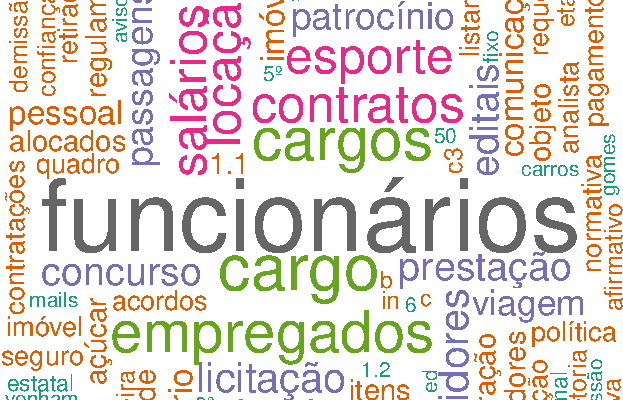
\includegraphics{markdown_v40_test_files/figure-latex/unnamed-chunk-66-3.pdf}

\begin{Shaded}
\begin{Highlighting}[]
\CommentTok{#View(head(plot_diretoria_palavras))}
\NormalTok{library(wordcloud2)}

\NormalTok{plot_diretorias_tf_dif = plot_diretoria_palavras %>%}
\NormalTok{  select(palavra, tf_idf, DIRETORIA) %>%}
\NormalTok{  mutate(palavra = reorder(palavra, tf_idf))}

\CommentTok{## DEE}
\CommentTok{#jpeg("XX_wordclou_tfidf_dir01_DEE.jpeg")}
\NormalTok{set.seed(233115)}
\NormalTok{plot_diretorias_tf_dif %>%}
\NormalTok{  filter(DIRETORIA == }\StringTok{"DEE"}\NormalTok{) %>%}
\NormalTok{  top_n(150, tf_idf) %>%}
\NormalTok{  wordcloud2(shuffle = TRUE, }
\NormalTok{             color = }\StringTok{"random-dark"}\NormalTok{,}
\NormalTok{             shape = }\StringTok{"circle"}\NormalTok{)}

\CommentTok{## DGC}
\CommentTok{#jpeg("XX_wordclou_tfidf_dir01_DGC.jpeg")}
\NormalTok{set.seed(233115)}
\NormalTok{plot_diretorias_tf_dif %>%}
\NormalTok{  filter(DIRETORIA == }\StringTok{"DGC"}\NormalTok{) %>%}
\NormalTok{  top_n(150, tf_idf) %>%}
\NormalTok{  wordcloud2()}

\CommentTok{## DEA}
\CommentTok{#jpeg("XX_wordclou_tfidf_dir01_DEA.jpeg")}
\NormalTok{set.seed(233115)}
\NormalTok{plot_diretorias_tf_dif %>%}
\NormalTok{  filter(DIRETORIA == }\StringTok{"DEA"}\NormalTok{) %>%}
\NormalTok{  top_n(150, tf_idf) %>%}
\NormalTok{  wordcloud2()}

\CommentTok{## DPG}
\CommentTok{#jpeg("XX_wordclou_tfidf_dir04_DPG.jpeg")}
\NormalTok{set.seed(233115)}
\NormalTok{plot_diretorias_tf_dif %>%}
\NormalTok{  filter(DIRETORIA == }\StringTok{"DPG"}\NormalTok{) %>%}
\NormalTok{  top_n(150, tf_idf) %>%}
\NormalTok{  wordcloud2()}

\CommentTok{## OUTROS}
\CommentTok{#jpeg("XX_wordclou_tfidf_dir01_OUTROS.jpeg")}
\NormalTok{set.seed(233115)}
\NormalTok{plot_diretorias_tf_dif %>%}
\NormalTok{  filter(DIRETORIA == }\StringTok{"OUTROS"}\NormalTok{) %>%}
\NormalTok{  top_n(150, tf_idf) %>%}
\NormalTok{  wordcloud2()}
\end{Highlighting}
\end{Shaded}

--\textgreater{}

\#\#\#\# Nuvem de palavras por diretoria - s/ steeming e/ou remoção de
stopwords - bigram

\texttt{r\ \ \ plot\_diretorias\_tf\_dif\_bigram\ =\ DB\ \%\textgreater{}\%\ \ \ select(DESCRI\_PEDIDO,DIRETORIA)\ \%\textgreater{}\%\ \ \ unnest\_tokens(BIGRAM,\ DESCRI\_PEDIDO,\ token\ =\ "ngrams",\ n\ =\ 2)\ \%\textgreater{}\%\ \ \ count(DIRETORIA,\ BIGRAM,\ sort\ =\ TRUE)\ \%\textgreater{}\%\ \ \ bind\_tf\_idf(BIGRAM,\ DIRETORIA,\ n)\ \%\textgreater{}\%\ \ \ arrange(desc(tf\_idf))\ \%\textgreater{}\%\ \ \ mutate(BIGRAM\ =\ factor(BIGRAM,\ levels\ =\ rev(unique(BIGRAM))))\ \%\textgreater{}\%\ \ \ mutate(DIRETORIA\ =\ factor(DIRETORIA,levels=c("DEA","DEE","DGC","DPG","OUTROS")))\ \%\textgreater{}\%\ \ \ select(BIGRAM,\ tf\_idf,\ DIRETORIA)}

\begin{Shaded}
\begin{Highlighting}[]
\NormalTok{## DEE}
\CommentTok{#jpeg("XX_wordclou_tfidf_dir01_DEE.jpeg")}
\NormalTok{nuvem1.}\DecValTok{2}\NormalTok{ =}\StringTok{ }
\StringTok{  }\NormalTok{plot_diretorias_tf_dif_bigram }\OperatorTok
\StringTok{  }\KeywordTok{filter}\NormalTok{(DIRETORIA }\OperatorTok{==}\StringTok{ "DEE"}\NormalTok{) }\OperatorTok
\StringTok{  }\KeywordTok{select}\NormalTok{(}\OperatorTok{-}\NormalTok{DIRETORIA, }\DataTypeTok{word =}\NormalTok{ BIGRAM,}\DataTypeTok{freq =}\NormalTok{ tf_idf) }\OperatorTok
\StringTok{  }\CommentTok{#top_n(150, freq) %>%}
\StringTok{  }\KeywordTok{as.data.frame}\NormalTok{() }

\KeywordTok{set.seed}\NormalTok{(}\DecValTok{231321}\NormalTok{)}
\KeywordTok{wordcloud}\NormalTok{(}\DataTypeTok{words =}\NormalTok{ nuvem1.}\DecValTok{2}\OperatorTok{$}\NormalTok{word, }\DataTypeTok{freq =}\NormalTok{ nuvem1.}\DecValTok{2}\OperatorTok{$}\NormalTok{freq, }\DataTypeTok{min.freq =} \FloatTok{0.2}\NormalTok{,}
          \DataTypeTok{max.words=}\DecValTok{250}\NormalTok{, }\DataTypeTok{random.order=}\OtherTok{FALSE}\NormalTok{, }\DataTypeTok{rot.per=}\FloatTok{0.35}\NormalTok{, }
          \DataTypeTok{colors=}\KeywordTok{brewer.pal}\NormalTok{(}\DecValTok{10}\NormalTok{, }\StringTok{"Dark2"}\NormalTok{))}
\end{Highlighting}
\end{Shaded}

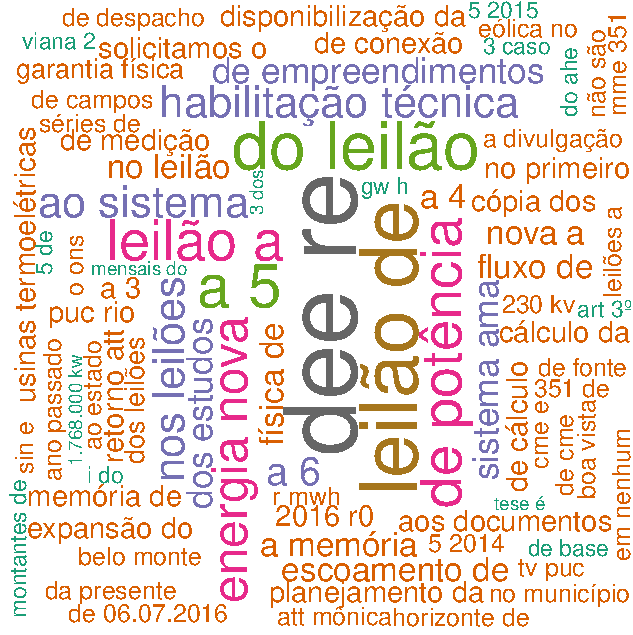
\includegraphics{markdown_v40_test_files/figure-latex/wordcloud_onegram_DIR01_semstopwords-1.pdf}

\begin{Shaded}
\begin{Highlighting}[]
\NormalTok{## DEA}
\CommentTok{#jpeg("XX_wordclou_tfidf_dir03_DEA.jpeg")}
\NormalTok{nuvem3.}\DecValTok{2}\NormalTok{ =}\StringTok{ }
\StringTok{  }\NormalTok{plot_diretorias_tf_dif_bigram }\OperatorTok
\StringTok{  }\KeywordTok{filter}\NormalTok{(DIRETORIA }\OperatorTok{==}\StringTok{ "DEA"}\NormalTok{) }\OperatorTok
\StringTok{  }\KeywordTok{select}\NormalTok{(}\OperatorTok{-}\NormalTok{DIRETORIA, }\DataTypeTok{word =}\NormalTok{ BIGRAM,}\DataTypeTok{freq =}\NormalTok{ tf_idf) }\OperatorTok
\StringTok{  }\CommentTok{#top_n(150, freq) %>%}
\StringTok{  }\KeywordTok{as.data.frame}\NormalTok{() }

\KeywordTok{set.seed}\NormalTok{(}\DecValTok{543453}\NormalTok{)}
\KeywordTok{wordcloud}\NormalTok{(}\DataTypeTok{words =}\NormalTok{ nuvem3.}\DecValTok{2}\OperatorTok{$}\NormalTok{word, }\DataTypeTok{freq =}\NormalTok{ nuvem3.}\DecValTok{2}\OperatorTok{$}\NormalTok{freq, }\DataTypeTok{min.freq =} \FloatTok{0.2}\NormalTok{,}
          \DataTypeTok{max.words=}\DecValTok{250}\NormalTok{, }\DataTypeTok{random.order=}\OtherTok{FALSE}\NormalTok{, }\DataTypeTok{rot.per=}\FloatTok{0.35}\NormalTok{, }
          \DataTypeTok{colors=}\KeywordTok{brewer.pal}\NormalTok{(}\DecValTok{10}\NormalTok{, }\StringTok{"Dark2"}\NormalTok{))}
\end{Highlighting}
\end{Shaded}

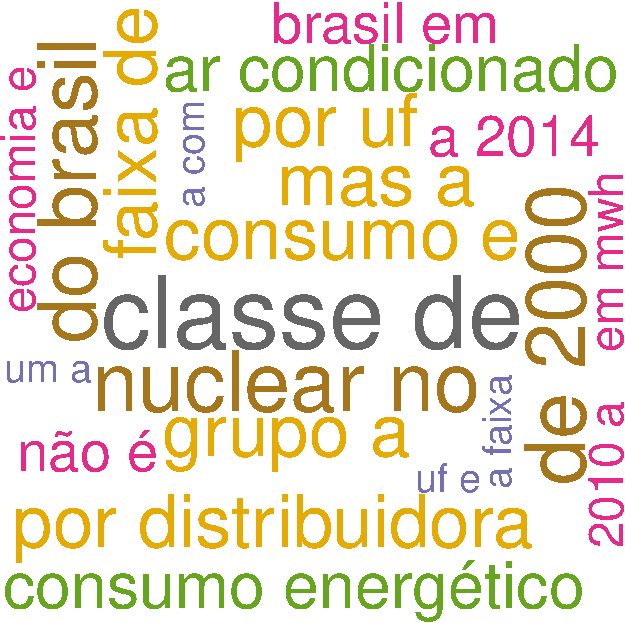
\includegraphics{markdown_v40_test_files/figure-latex/wordcloud_onegram_DIR03_semstopwords-1.pdf}

\begin{Shaded}
\begin{Highlighting}[]
\NormalTok{## OUTROS}
\CommentTok{#jpeg("XX_wordclou_tfidf_dir05_OUTROS.jpeg")}
\NormalTok{nuvem5.}\DecValTok{2}\NormalTok{ =}\StringTok{ }
\StringTok{  }\NormalTok{plot_diretorias_tf_dif_bigram }\OperatorTok
\StringTok{  }\KeywordTok{filter}\NormalTok{(DIRETORIA }\OperatorTok{==}\StringTok{ "OUTROS"}\NormalTok{) }\OperatorTok
\StringTok{  }\KeywordTok{select}\NormalTok{(}\OperatorTok{-}\NormalTok{DIRETORIA, }\DataTypeTok{word =}\NormalTok{ BIGRAM,}\DataTypeTok{freq =}\NormalTok{ tf_idf) }\OperatorTok
\StringTok{  }\CommentTok{#top_n(150, freq) %>%}
\StringTok{  }\KeywordTok{as.data.frame}\NormalTok{() }

\KeywordTok{set.seed}\NormalTok{(}\DecValTok{75437}\NormalTok{)}
\KeywordTok{wordcloud}\NormalTok{(}\DataTypeTok{words =}\NormalTok{ nuvem5.}\DecValTok{2}\OperatorTok{$}\NormalTok{word, }\DataTypeTok{freq =}\NormalTok{ nuvem5.}\DecValTok{2}\OperatorTok{$}\NormalTok{freq, }\DataTypeTok{min.freq =} \FloatTok{0.1}\NormalTok{,}
          \DataTypeTok{max.words=}\DecValTok{250}\NormalTok{, }\DataTypeTok{random.order=}\OtherTok{FALSE}\NormalTok{, }\DataTypeTok{rot.per=}\FloatTok{0.35}\NormalTok{, }
          \DataTypeTok{colors=}\KeywordTok{brewer.pal}\NormalTok{(}\DecValTok{10}\NormalTok{, }\StringTok{"Dark2"}\NormalTok{))}
\end{Highlighting}
\end{Shaded}

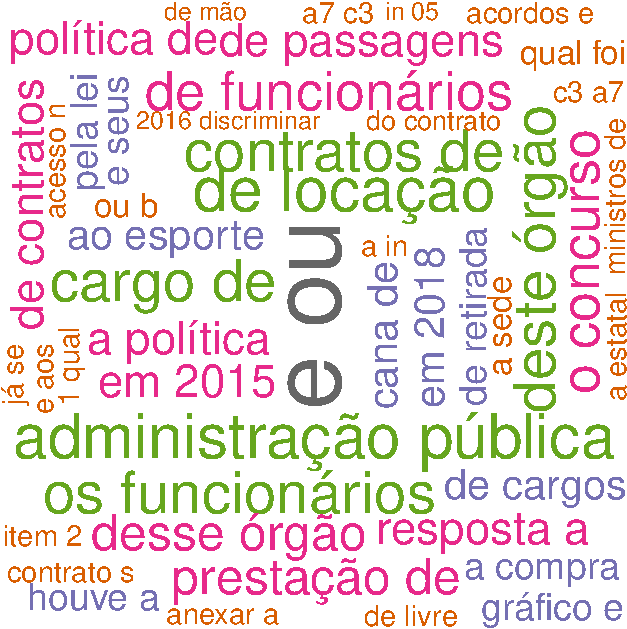
\includegraphics{markdown_v40_test_files/figure-latex/wordcloud_onegram_DIR05_semstopwords-1.pdf}

\section{MODELAGEM - APLICAÇÃO E
RESULTADOS}\label{modelagem---aplicacao-e-resultados}


\end{document}
